\lhead{\begin{tikzpicture}[remember picture, overlay]
    \node [anchor=100,inner sep=0] (imagenIZQUIERDA) at (current page header area.north){
\includegraphics[width=18cm]{img/Encabezado.PNG}};
    \end{tikzpicture}}
    \rhead{Autor: Llamas-Nuñez}
    \rfoot{\begin{tikzpicture}[remember picture, overlay]
    \node [anchor=140,inner sep=0] (imagenDERECHA) at (current page footer area.south){
\includegraphics[width=18cm]{img/Foot.PNG}};
    \end{tikzpicture}}
    %----------------------------------------------------------------------------------------
    \lfoot{ \thepage}
    % \renewcommand{\labelenumi}{\alph{enumi}.)} 
    %----------------------------------------------------------------------------------------
    %----------------------------------------------------------------------------------------
    %	TITLE SECTION
    %----------------------------------------------------------------------------------------
    
    \setlength{\droptitle}{-5\baselineskip} % Move the title up
    \title{\textbf{ Estudio de tiempos y movimientos en el ensamble de un circuito electrónico utilizando diferentes métodos para su optimización} } % Article title
    
     \author{ 
     \textsc{Llamas Nuñez, Ana Valeria}\\ 
    %  Afiliación:
     \texttt{ Instituto Tecnológico de Querétaro } \\ 
     \texttt{Tecnológico Nacional de México  } \\ 
     \texttt{Querétaro, México}\\ 
     \texttt{ llamasnunezanavaleria@gmail.com } 
     \and 
     \textsc{Ángeles Hurtado, Luis Alberto}\\ 
    %  Afiliación:
     \texttt{ Instituto Tecnológico de Querétaro } \\ 
     \texttt{ Tecnológico Nacional de México } \\ 
     \texttt{ Querétaro, México }\\ 
     \texttt{ alb3rto.ah@gmail.com } 
    }
    
    
    %----------------------------------------------------------------------------------------
    
    % \begin{document}
    
    % Print the title
    \maketitle
    \thispagestyle{fancy}
    
    %----------------------------------------------------------------------------------------
    %	ARTICLE CONTENTS
    %----------------------------------------------------------------------------------------
    
    % \section*{Resumen}
    % \textit{Palabras clave:}
    % El resumen (ancho de página) deberá contener entre 100 y 200 palabras tipo Adobe Devangari 11 puntos.
    
    \begin{abstract}
    \noindent 
     
    
    \end{abstract}
    % 
    % 
    \textbf{\textit{Palabras clave}}: {First keyword should be the corresponding to the research area according with the authors guide. Maximum of 6 keywords.}
    % \keywords{First keyword should be the corresponding to the research area according with the authors guide. Maximum of 6 keywords.}
    
    \section{Introducción}
    
    
    % Define estudio de tiempos y movimientos
    % define que es ensamble
    % define que es circuito electronico
    % define el metodo de tiempos predeterminados
    % define optimización
\begin{itemize}
    \item El estudio de tiempos y movimientos es el análisis de medios, materiales e instalación el cual nos permite encontrar la forma más económica de realizar el trabajo, estandarizando las herramientas que se han de utilizar para ejecutar el método de acción . Lo cual para llevar a cabo este proyecto, nos basamos en el estudio de tiempos y movimientos para aprender, comprender, ejecutar y  mejorar el análisis que se efectuara durante las labores, permitiéndonos analizar la secuencia de eventos que ocurren durante la acción  realizada. 
Dicho análisis se identificará durante el proceso de manufactura en el cual dos o más materiales se unen para formar un ensamble el cual su función es generar un circuito electrónico que nos permite realizar una secuencia fijando una metodología, del proceso cuya estructura es basada en crear un recorrido por el cual pueda viajar la información. para que esta se generare, transmita, reciba y almacene fijando así cuya importancia estratégica nos sirve para poder efectuar la optimización de procesos y buscar la mejora continua. En pocas palabras nos sirve para identificar el conjunto de reglas o métodos para determinar con anticipación la secuencia de sucesos, a esta acción se le conoce como método de tiempos predeterminados. De modo que  llevando acabo  esta estructura nos permite identificar de manera más efectiva los procesos para utilización de ejecución en el área de ingeniería de procesos de producción, calidad y manufactura.  

        
    
    \end{itemize}
    % 
    % 
    \section{Justificación}
    
    \begin{itemize}
        \item En base al Estudio de Trabajo durante este proyecto se busca mejorar y optimizar los tiempos y movimientos que realizara el operador buscando así mejorar la productividad, según Kanawaty en su obra «Introducción al estudio del trabajo» lo define así: "El estudio del trabajo es el examen sistemático de los métodos para realizar actividades con el fin de mejorar la utilización eficaz de los recursos y de establecer normas de rendimiento con respecto a las actividades que se están realizando". Por lo tanto, este tiene como objetivo evaluar de qué manera se está llevando a cabo el trabajo para así facilitar o transformar el método con el cual está trabajando para disminuir el tiempos y movimientos innecesarios. Para así dentro de este buscar la manera más económica y eficaz de realizar el trabajo.
 En la actualidad, se demanda una eficiencia cada vez mayor en la producción y productividad debido al crecimiento de la industria. Los fabricantes necesitan identificar sus procesos de producción de manera que les permitan realizar con exactitud, efectividad y de forma continua.
 Para lograr esto, el uso de técnicas avanzadas de estudio de tiempos y movimientos durante el proceso de ensamblaje es fundamental. Se necesita una comprensión profunda de cómo se realizan las tareas y los movimientos necesarios para completar el ensamble. Esto incluye la evaluación de la eficiencia del proceso, el análisis de movimientos y el uso de tecnologías de seguimiento de tiempos. Además, se necesita una optimización continua de los métodos aplicados para reducir los tiempos de producción, minimizar los errores y mejorar la calidad del producto final.
 Estos procesos se siguen implementando en diferentes sectores industriales, tales como el sector automotriz, aeronáutico, alimenticio, farmacéutico, por mencionar algunos de ellos

        \item Debe de tener Referencias científicas, URL, tesis, etc.
    \end{itemize}
    % 
    % 
    \section{Descripción del problema}
    \begin{itemize}
        \item Se tiene como objetivo diseñar, mejorar e integrar sistemas productivos para ensamblar el circuito electrónico, aplicando tecnologías para su optimización. Así como desarrollar e implementar sistemas de trabajo para aumentar la productividad. Para obtener resultados concretos utilizaremos sistemas de tiempos predeterminados para establecer estándares de trabajo que promuevan la eficiencia. Para garantizar una mayor aptitud este también incluirá la realización de muestreos de trabajo para la estandarización dentro del área operativa. 
    \end{itemize}
    
    \textbf{*La incógnita científica es el elemento cuya solución incrementa el conocimiento científico.}
    % 
    % 
    \section{Fundamentación teórica}
    
El estudio de métodos en el registro y examen crítico sistemático de los modos de realizar actividades, con el fin de efectuar mejoras.
Se examinarán de los métodos para realizar actividades con el fin de mejorar la utilización eficaz de los recursos y establecer normas de rendimiento con respecto a las actividades. El objetivo es evaluar la forma en que se está llevando a cabo el trabajo con el fin de facilitar o modificar el enfoque con el que está trabajando para reducir el tiempo y los movimientos innecesarios, a esto se le conoce como Sistema de Tiempos Predeterminados (STP). Esto se realizará en base a los principios de la ingeniería industrial los cuales proporcionan la base para entender cómo se pueden mejorar los procesos de producción mediante el análisis, estandarización y optimización de los tiempos y movimientos.
Se buscará establecer métodos de trabajo estándar para garantizar la uniformidad y la calidad en el proceso de ensamble. Esto implica definir pasos específicos para cada tarea, así como los tiempos y movimientos asociados a cada una de ellas. Para ello se buscara encontrar la mejor manera de llevar a cabo el ensamble con los recursos disponibles y  así se  centrara en analizar el tiempo requerido para llevar a cabo cada una de las actividades dentro del ensamble así como los movimientos físicos que realiza el operador durante el ensamble de circuitos electrónicos. Se busca identificar movimientos innecesarios que puedan ser eliminados o simplificados para mejorar la eficiencia.

    
    
    \begin{itemize}
        \item Se debe de retomar el tema que se planteo en la introducción, pero ahora profundizando para clarificar la incógnita científica y se pueda plantear la hipótesis.
        \item Se debe de retomar la descripción del problema, pero ahora a profundidad del (los) objeto(s) de estudio. 
        \item Se debe de profundizar en las metodologías que se ha usado para el estudio del tema.
        \item Referencias solo de artículos y libros científicos.
    \end{itemize}
    % 
    % 
    \section{Hipótesis}
    Si se implementa el Sistema de Tiempos Predeterminados en el Proyecto Integrador, lograremos aplicar la reducción de tiempo y movimientos, logrando así la forma más económica de hacer el trabajo ejecutando un plan de acción, alcanzando así plasmar todos los temas vistos dentro de la materia de Estudio del Trabajo II.
    
    %Es la suposición con fundamento científico relativa a la solución del problema, necesidad o de cómo se aprovecha la oportunidad con la incógnita científica y se fundamenta con: 1. Una suposición (en afirmativo o negativo) y ésta deberá vincularse con:
    %2. La fundamentación científica que deberá ser precisa 3. Una entidad de comparación para probar la suposición y
    %4. La variable con que se califica o cuantifica la comparación o se prueba la hipótesis.
    
    %\begin{itemize}
    %\item Se debe de identificar claramente la suposición científica
    %\item Se debe de identificar claramente el fundamento científico
    %\item Se debe identificar claramente la variable de respuesta
    %\item Se debe identifican claramente las realidades o modelos contrastantes
    %\item Se debe de establecer las variables asociadas, explicativas o que tienen relación funcional con la variable de respuesta
    %\end{itemize}
    % 
    % 
    \section{Objetivo}
    
    \begin{itemize}
        \item Diseñaré, mejoraré e integraré sistemas productivos de bienes y servicios aplicando tecnologías para su optimización
        \item Diseñaré, implementaré y mejoraré sistemas de trabajo para elevar la productividad
    \end{itemize}
    
    \subsection{Objetivos específicos }
    
    \begin{itemize}
    \item Desarrollar una guía de emergencia para analizar la instalación en la que se llevo acabo la experimentación.
     \item Analizar los métodos, materiales, herramientas e instalación utilizada o que se ha de utilizar en la ejecución del ensamble de un circuito electrónico.
    \item Se establecerá la forma más económica de realizar el trabajo.
    \item Normalizar los métodos, materiales, herramientas e instalaciones.
    \item Determinar exactamente el tiempo necesario para que una persona competente realice el trabajo con una marcha normal.
    \item Aplicar los sistemas de tiempos predeterminados como fundamento del estudio de tiempos para establecer estándares.
    \item Realizar el muestreo de trabajo para la estandarización en el área operativa.
        
    \end{itemize}
    
    % 
    % 
    \section{Cuerpo (Metodología, modelo matemático, etc.)}
    Durante esta investigación realizada mediante técnicas de observación y análisis estadístico. La recopilación de datos se efectuó en la ciudad de Querétaro, en las instalaciones del Instituto Tecnológico de Querétaro (ITQ), durante el periodo comprendido entre febrero y mayo de 2024.

    El estudio se enfocó en el montaje de una tarjeta electrónica utilizando software de diseño asistido por computadora. Se definieron las estructuras de todos los niveles del montaje, se establecieron los límites de potencia y control necesarios para desarrollar el diseño requerido, y finalmente, se seleccionó la opción más adecuada para su implementación.

    En la primera fase de la experimentación, se tomaron dos muestras continuas mediante una cámara de vídeo. Posteriormente, se aplicaron diversas metodologías para determinar el tiempo de ciclo y el tiempo estándar del proceso. Este enfoque permitió una evaluación precisa y detallada del montaje de la tarjeta electrónica, facilitando la identificación de áreas de mejora y optimización en el proceso productivo.
    %
    %
    \begin{figure}[H]
        \centering
        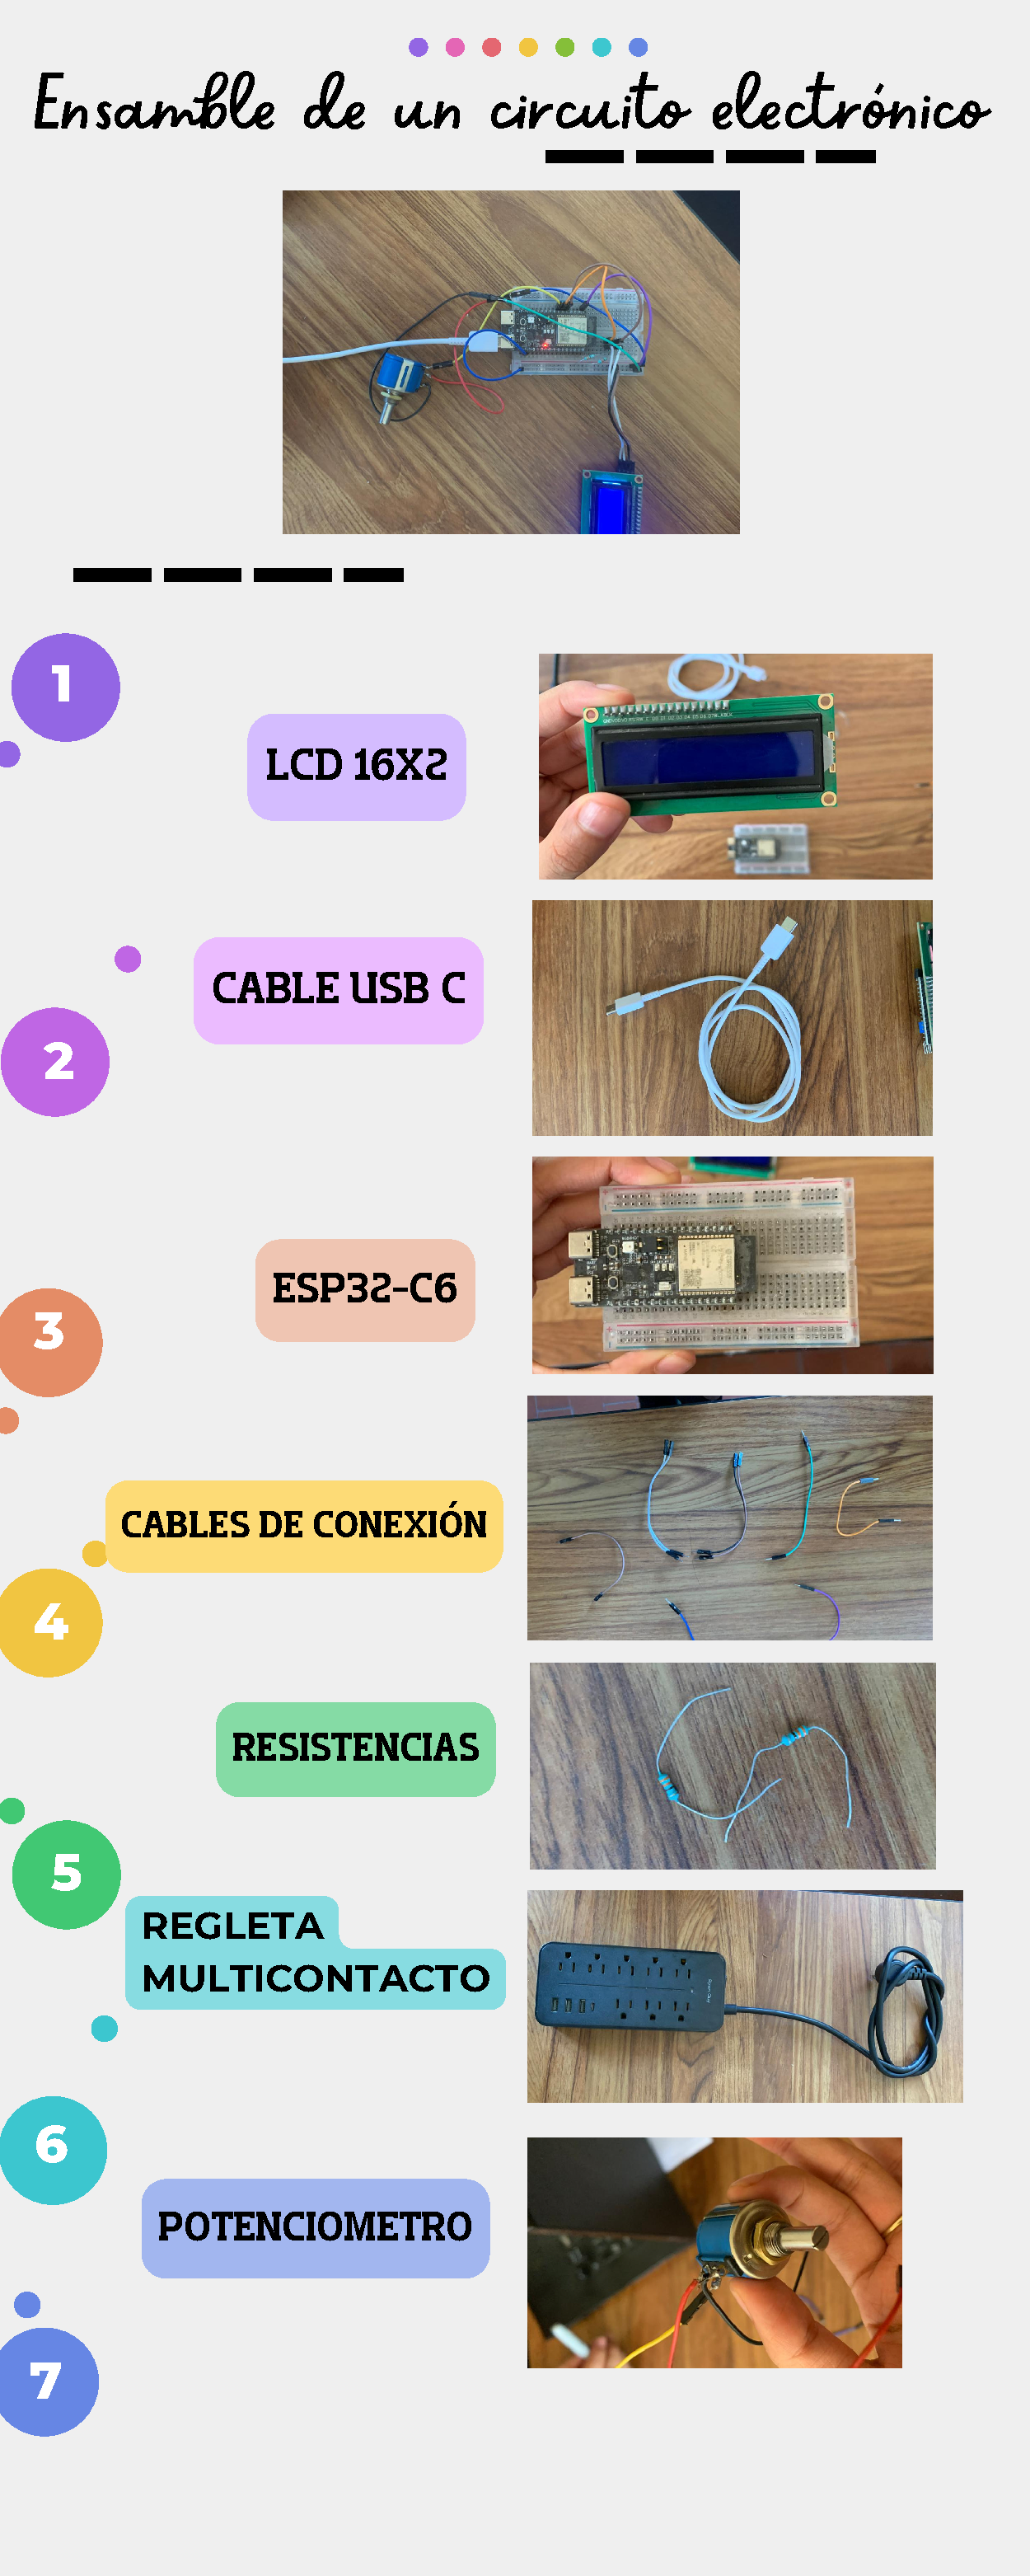
\includegraphics[trim = {25mm 50mm 20mm 140mm},clip,scale=0.3]{16/Img/materialesCE.pdf}
        \caption{Materiales}
        \label{fig:Materiales}
    \end{figure}
    % 
    % 
    
    % 
    % 
    \begin{figure}[H]
        \centering
        \includegraphics[trim = {10mm 10mm 10mm 10mm},clip,scale=0.150]{16/Img/cablesDeConexión.PDF}
        \caption{Cables de conexión}
        \label{fig:Cables de conexión}
    \end{figure}
    % 
    % 
    % 
    % 
    \begin{figure}[H]
        \centering
        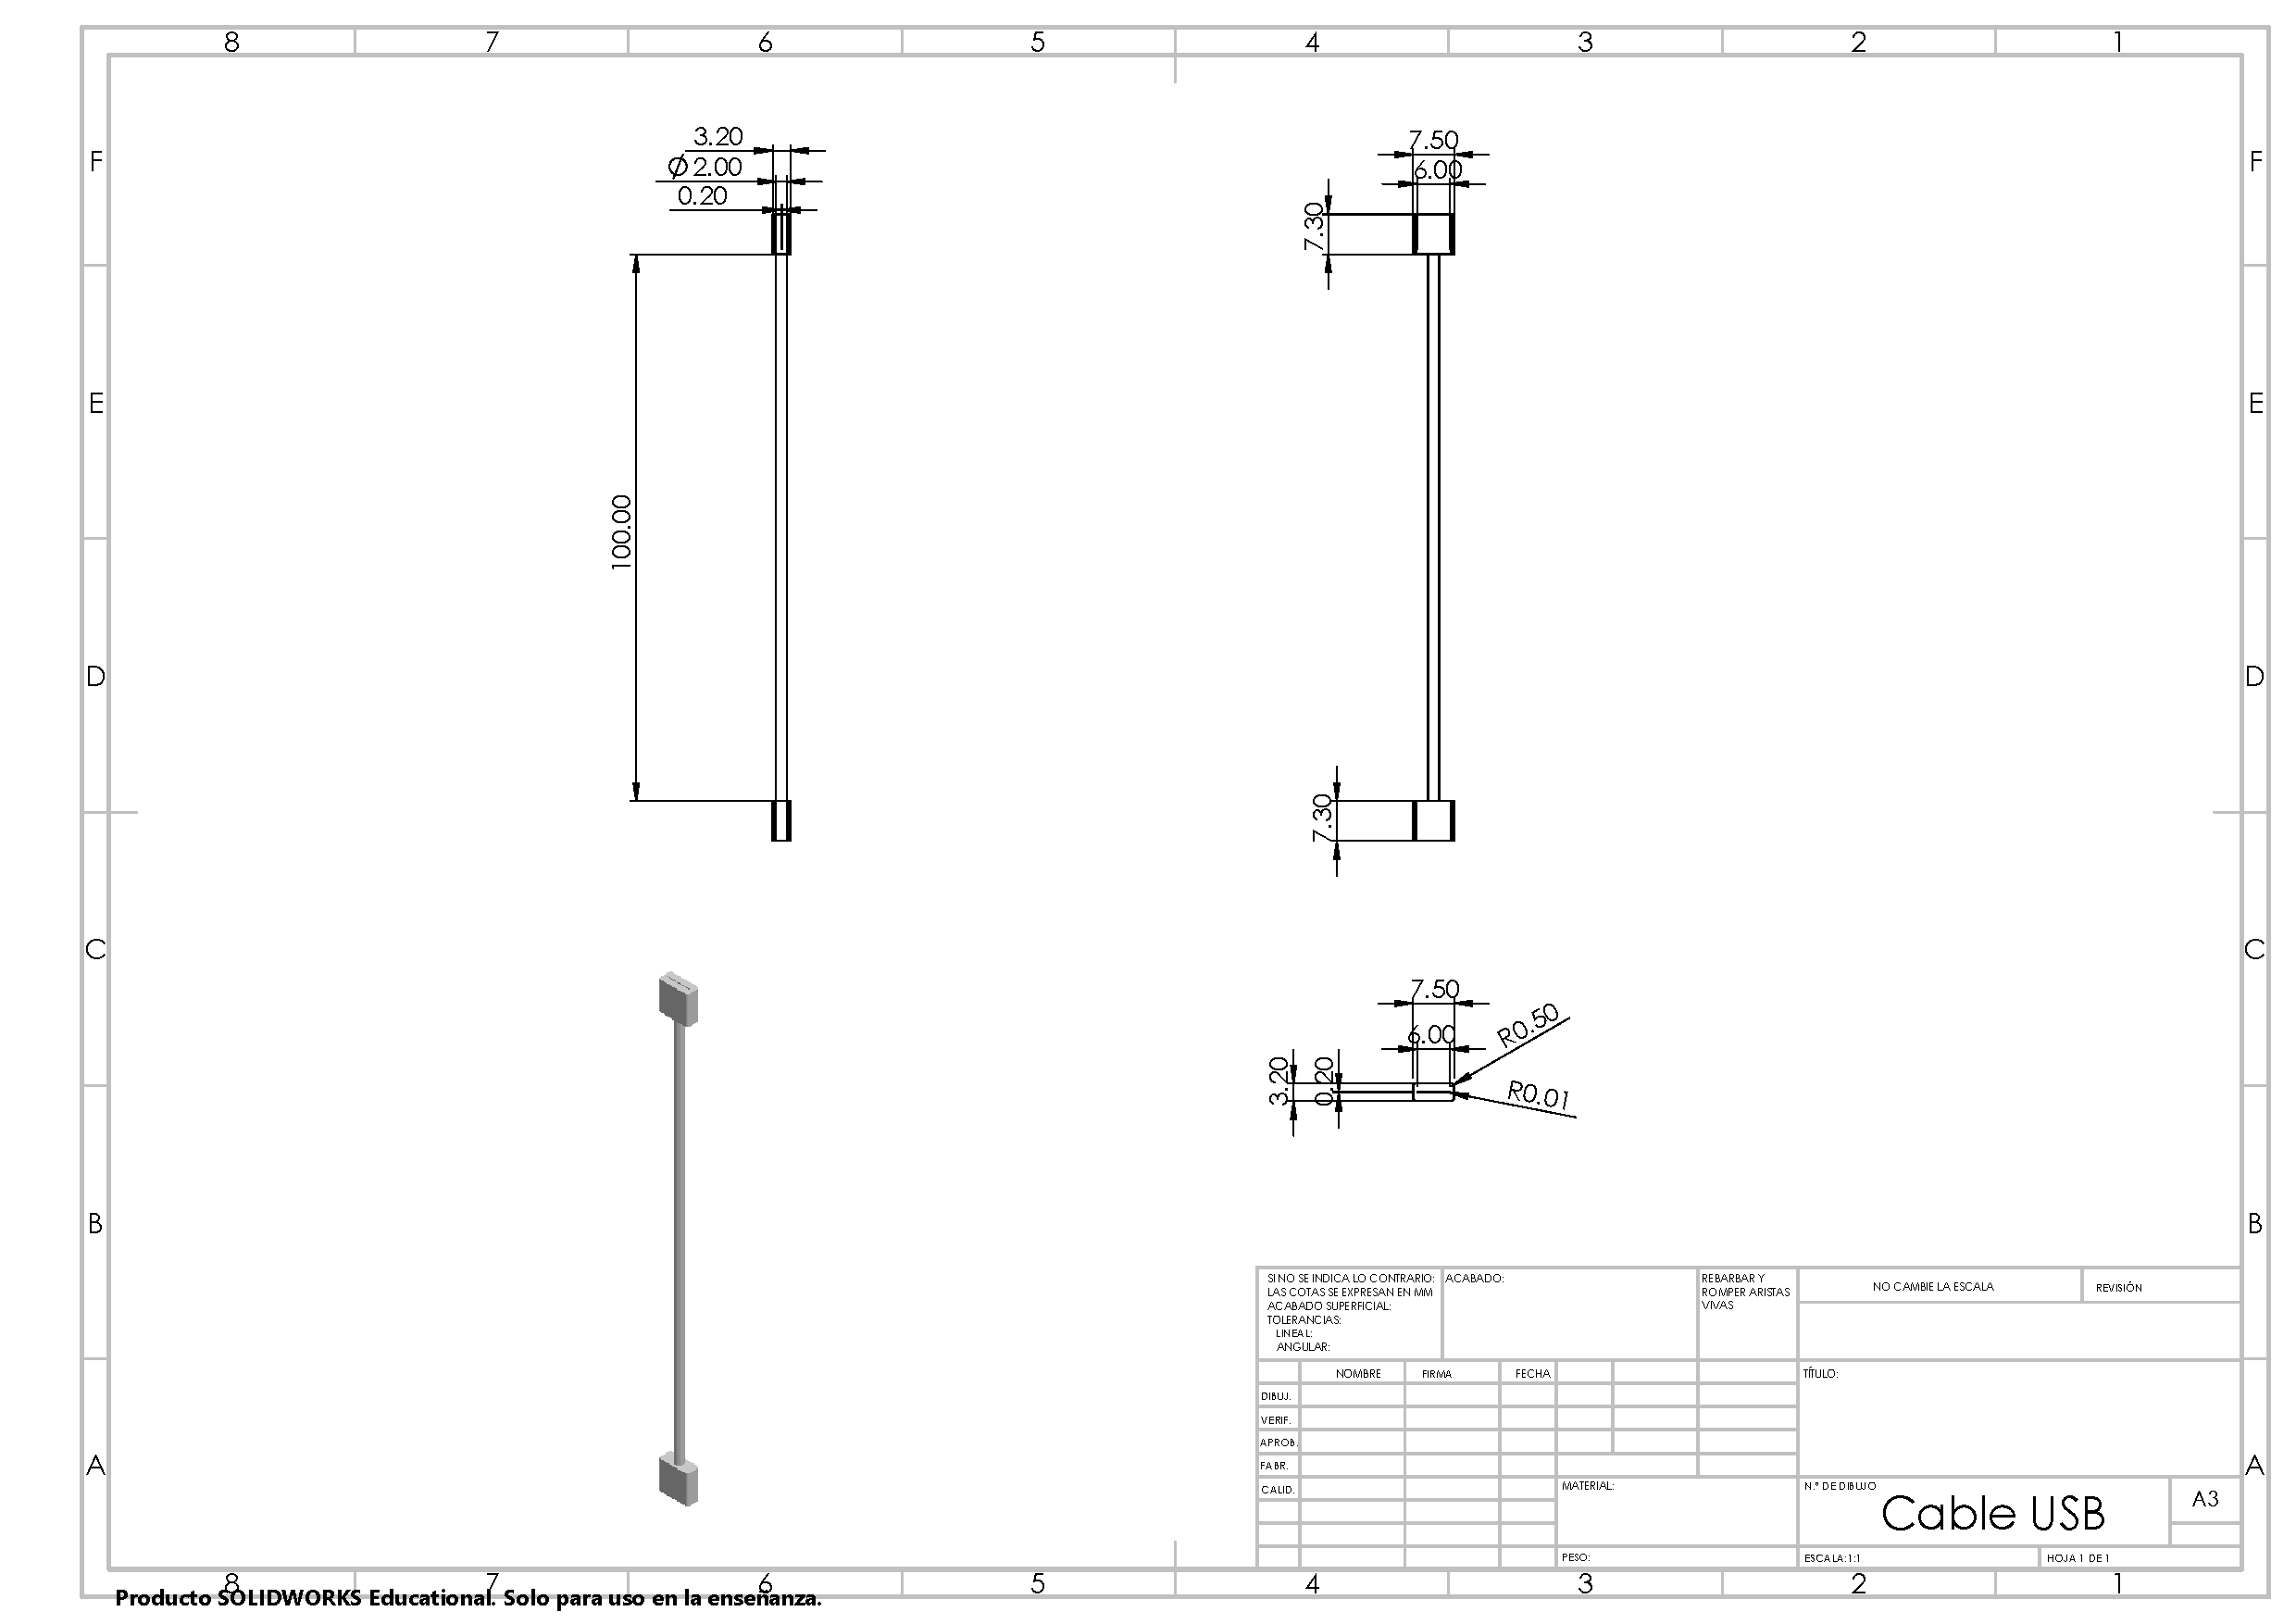
\includegraphics[trim = {10mm 10mm 10mm 10mm},clip,scale=0.150]{16/Img/cableUSB.PDF}
        \caption{Cables USB}
        \label{fig:Cable USB}
    \end{figure}
    % 
    % 
    % 
    % 
    \begin{figure}[H]
        \centering
        \includegraphics[trim = {10mm 10mm 10mm 10mm},clip,scale=0.150]{16/Img/eSP32.PDF}
        \caption{ESP32-C6}
        \label{fig:ESP32-C6}
    \end{figure}
    % 
    % 
    % 
    % 
    \begin{figure}[H]
        \centering
        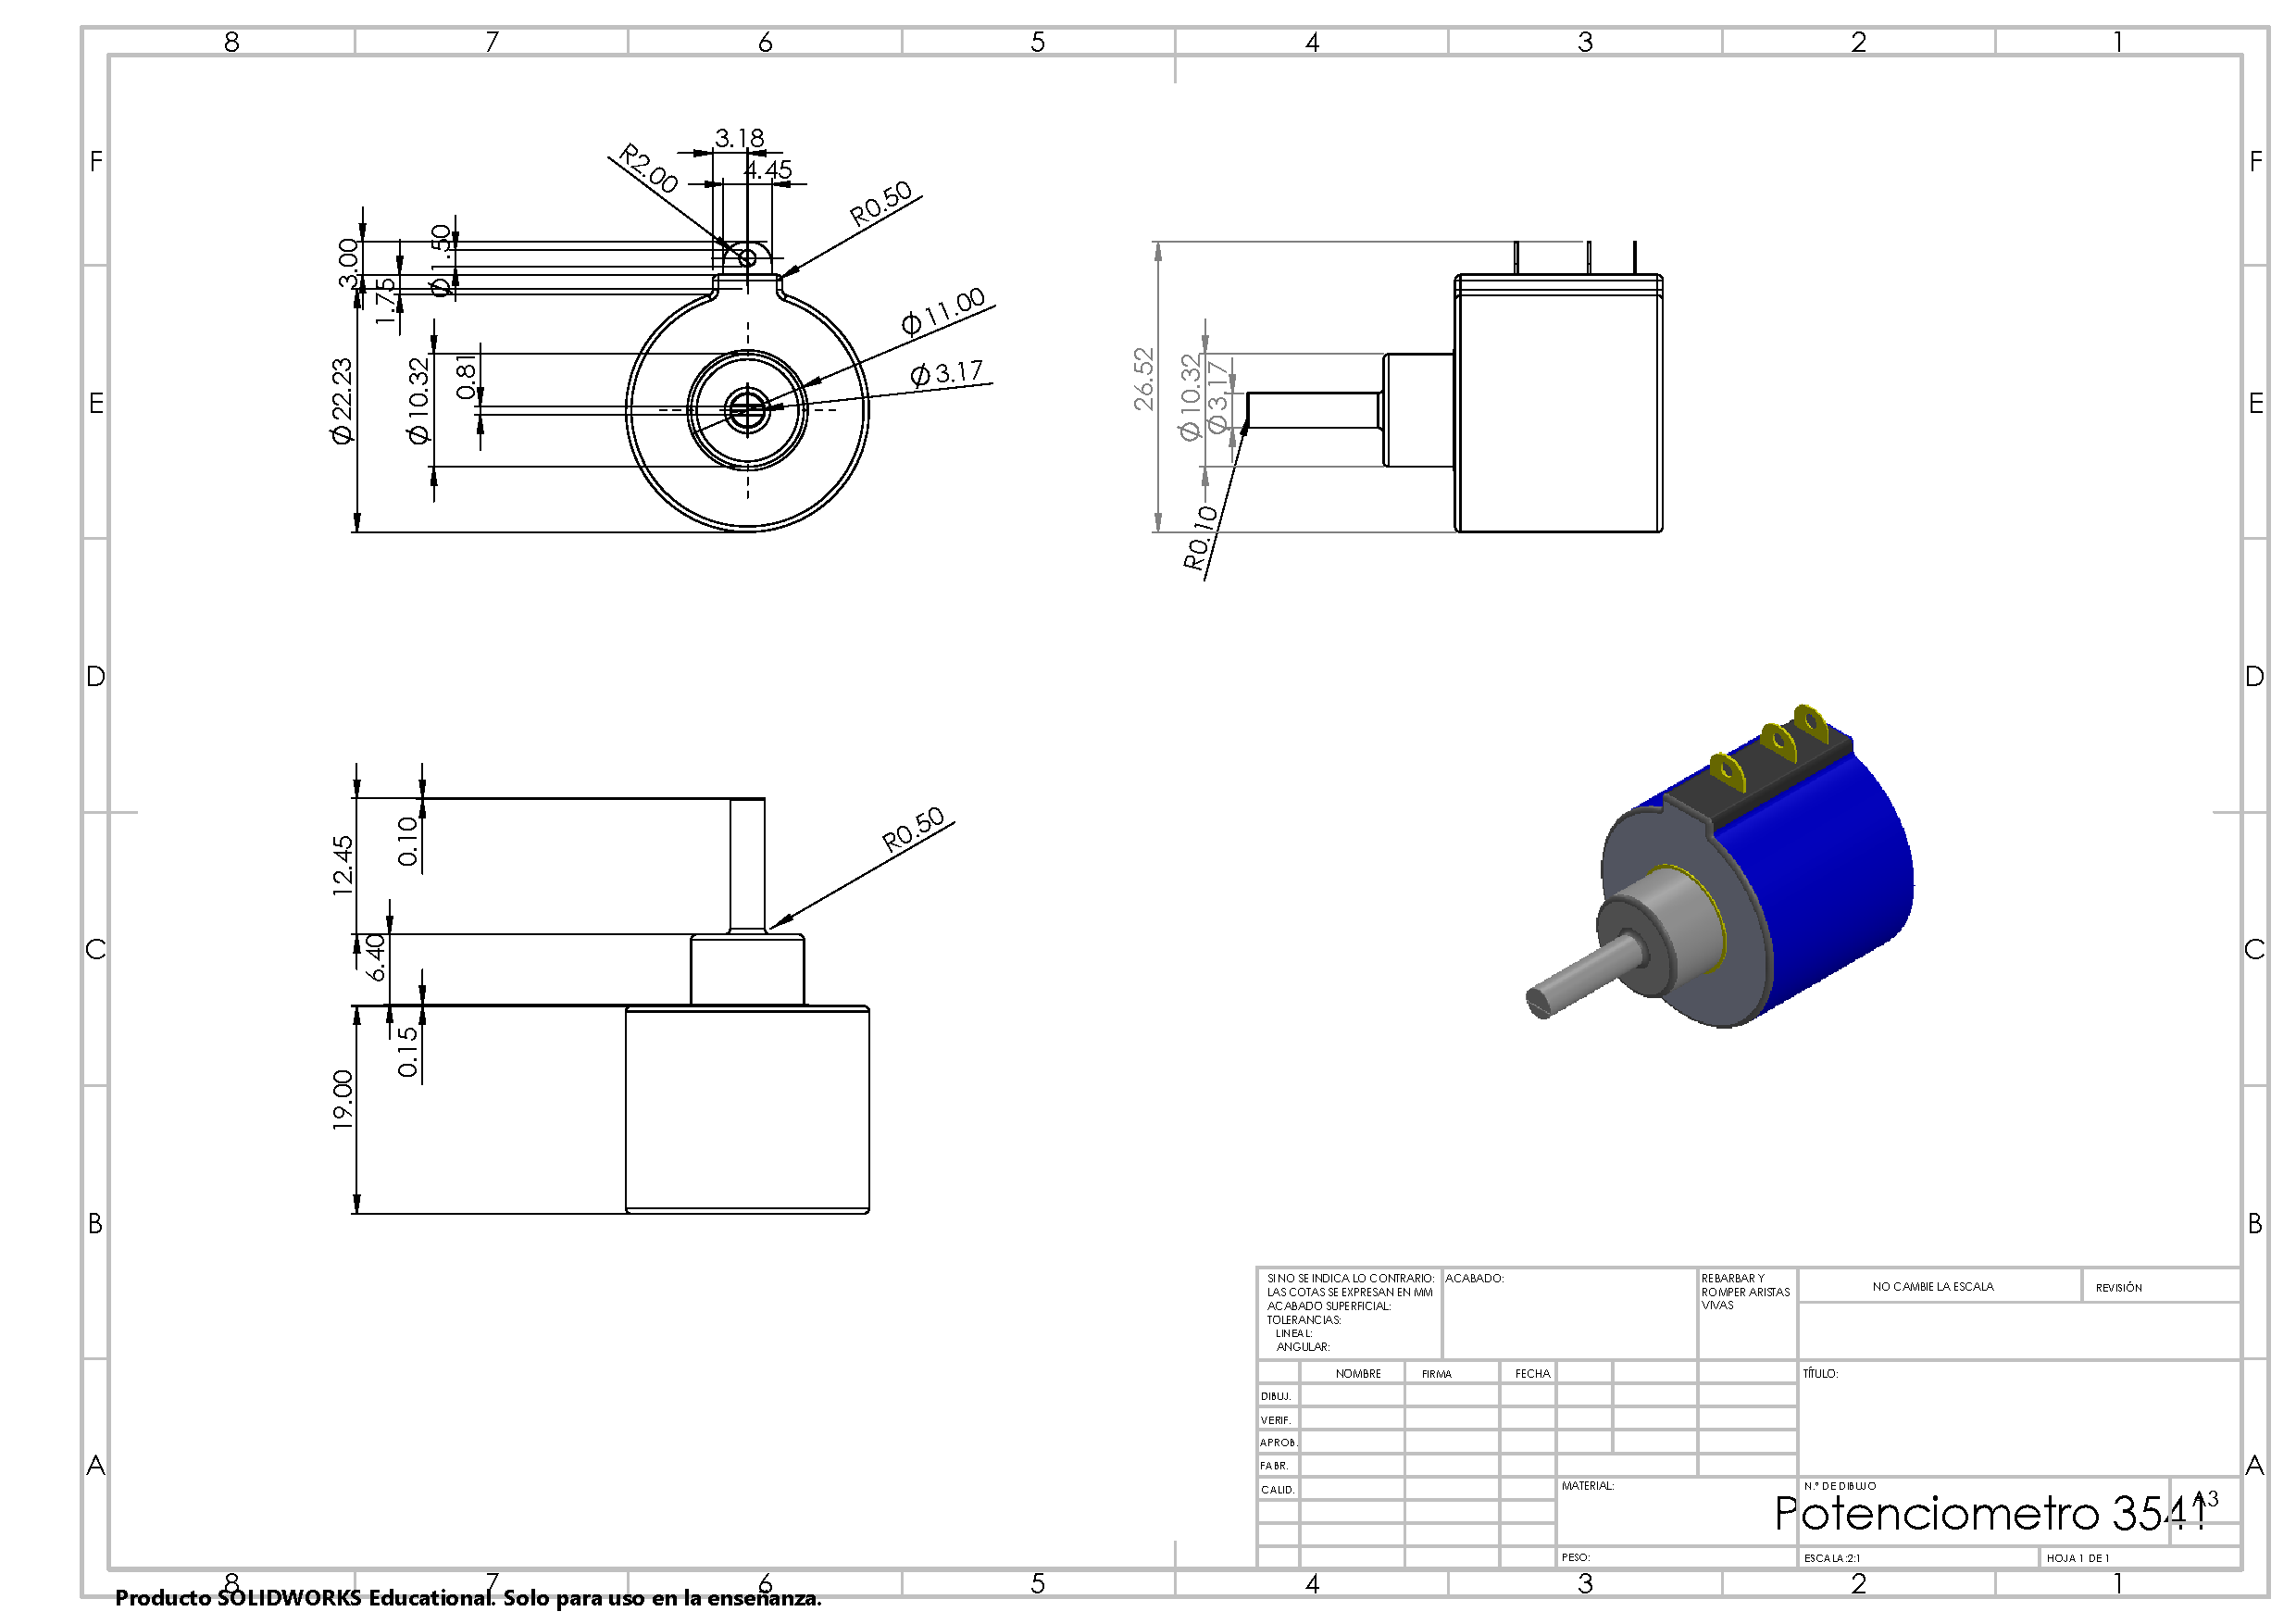
\includegraphics[trim = {10mm 10mm 10mm 10mm},clip,scale=0.150]{16/Img/potenciometro.PDF}
        \caption{Potenciometro}
        \label{fig:Potenciometro}
    \end{figure}
    % 
    % 
    % 
    % 
    \begin{figure}[H]
        \centering
        \includegraphics[trim = {10mm 10mm 10mm 10mm},clip,scale=0.150]{16/Img/cablesDeConexiónMM .PDF}
        \caption{Cable de conexión MM}
        \label{fig:Cable de conexión MM}
    \end{figure}
    % 
    % 
    % 
    % 
    \begin{figure}[H]
        \centering
        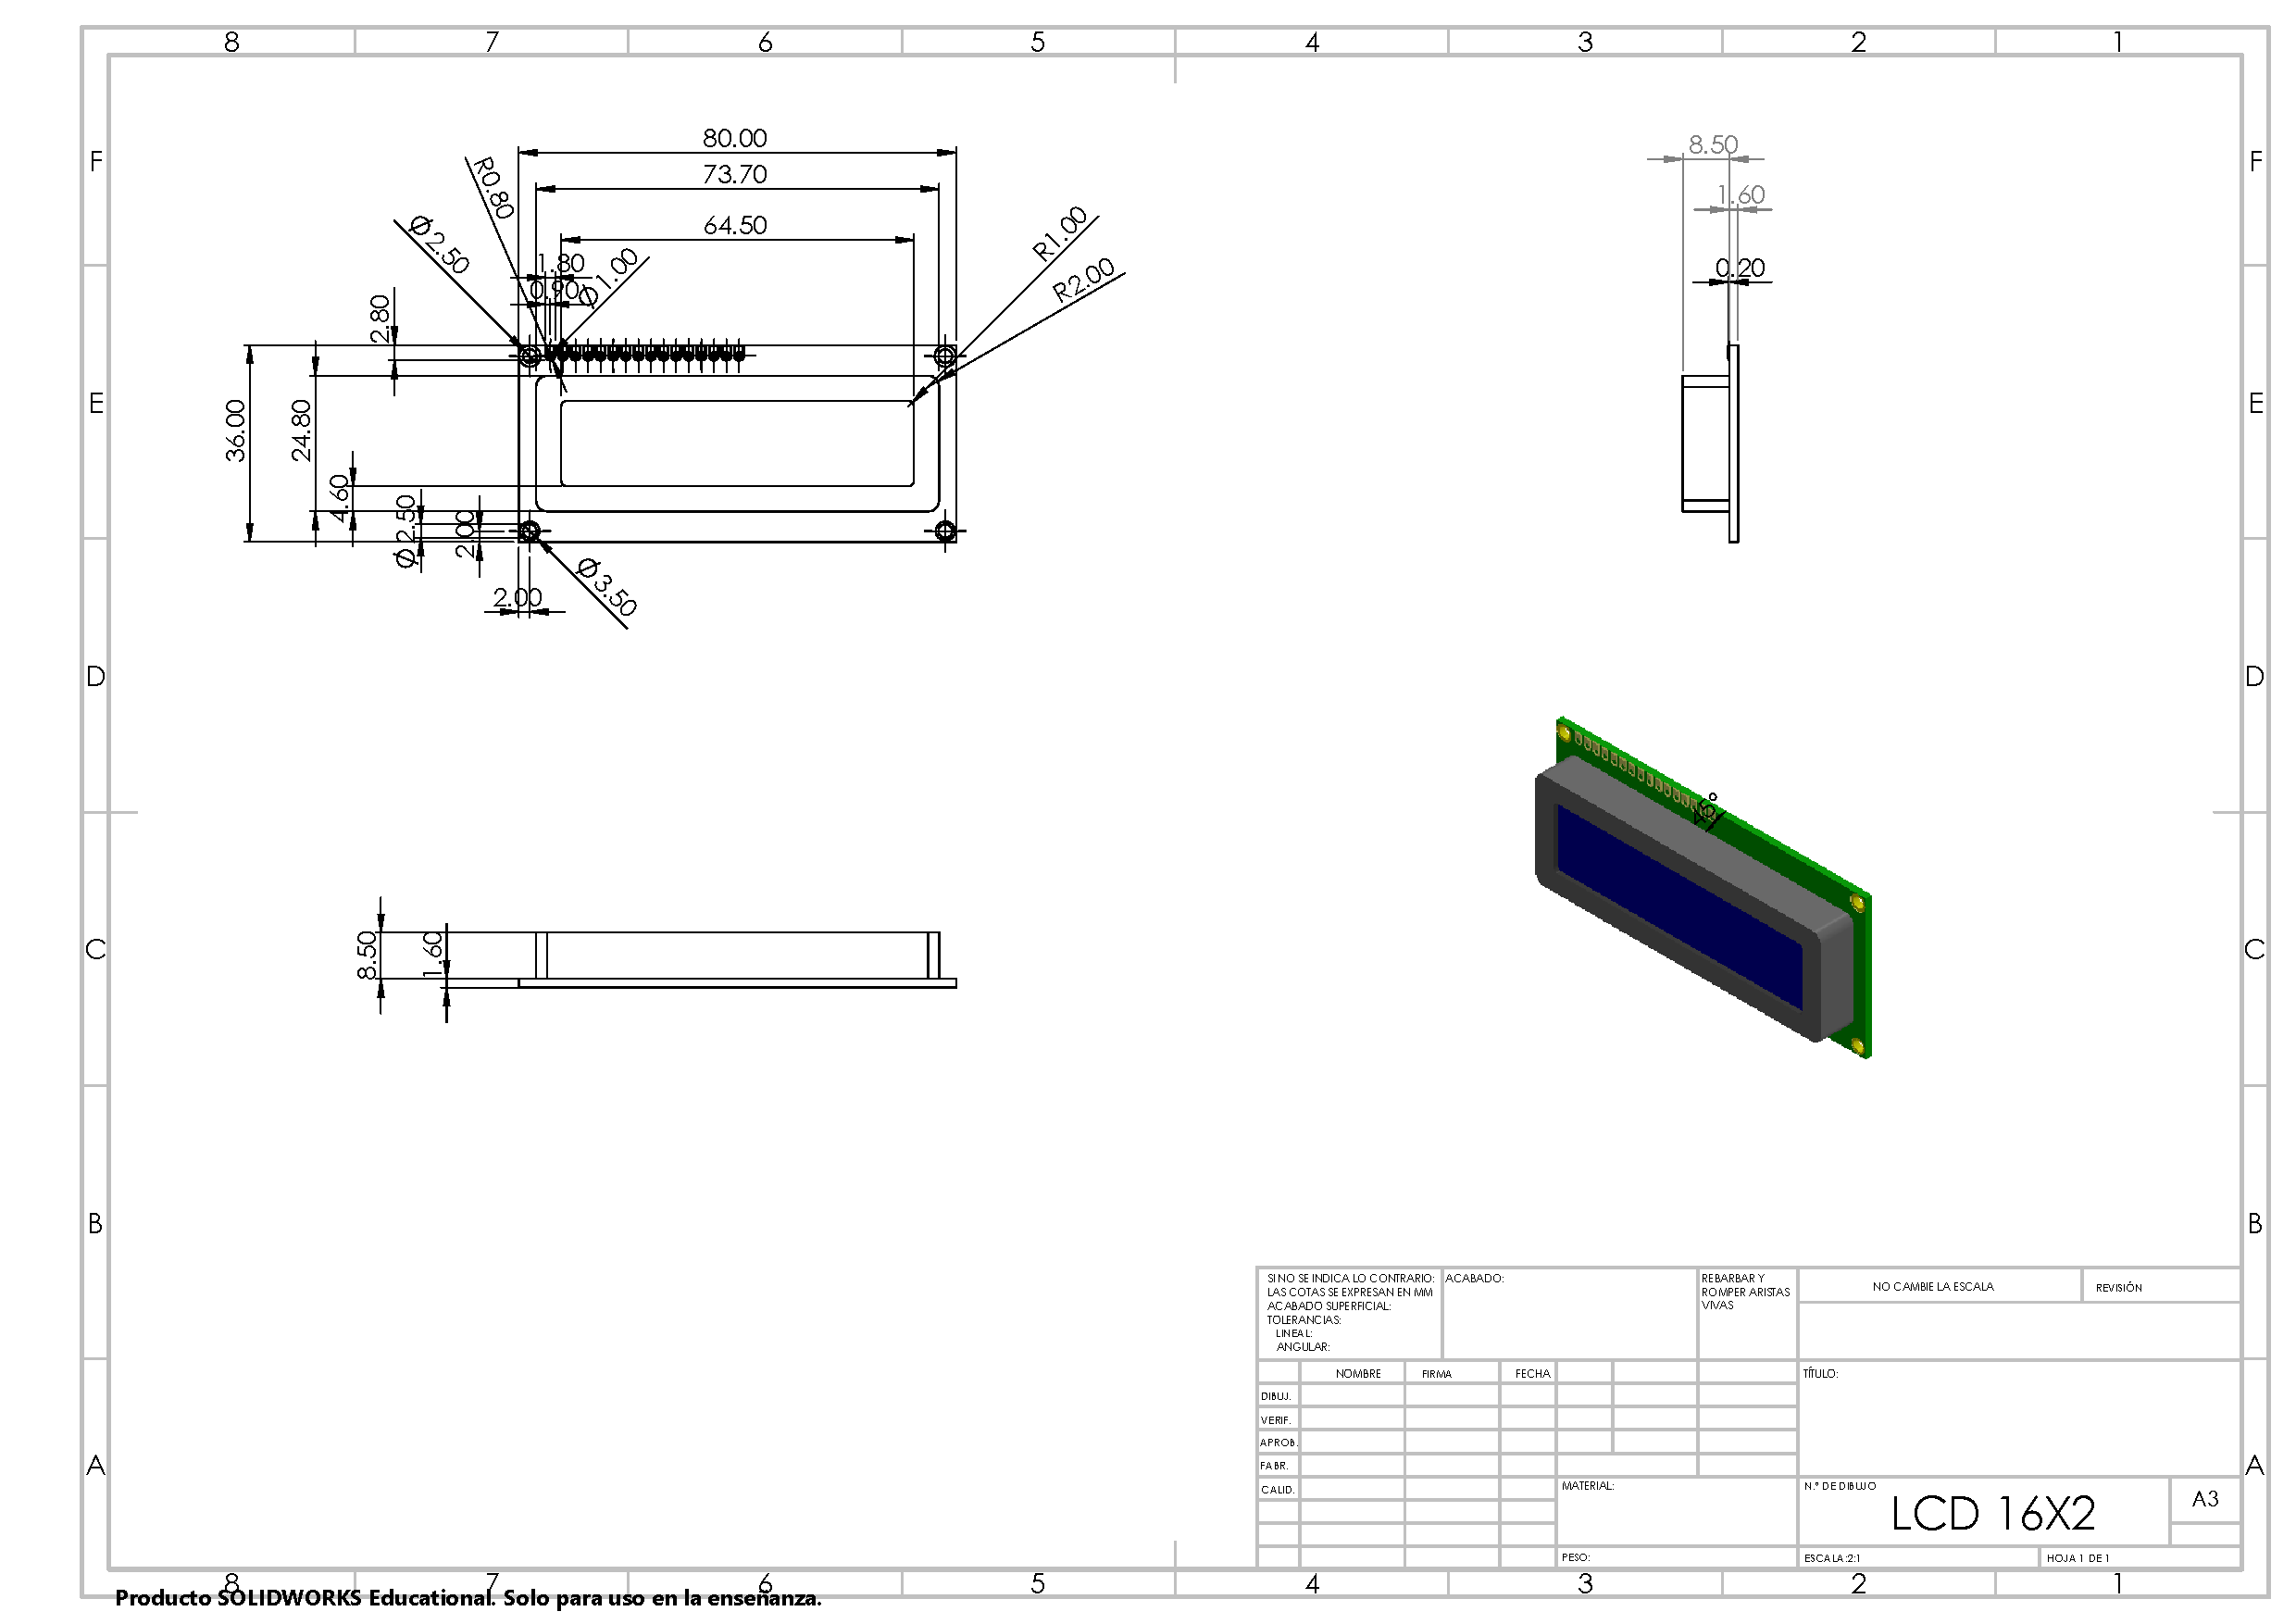
\includegraphics[trim = {10mm 10mm 10mm 10mm},clip,scale=0.150]{16/Img/lCD16X2.PDF}
        \caption{LCD 16X2}
        \label{fig:LCD 16X2}
    \end{figure}
    % 
    % 
    % 
    % 
    \begin{figure}[H]
        \centering
        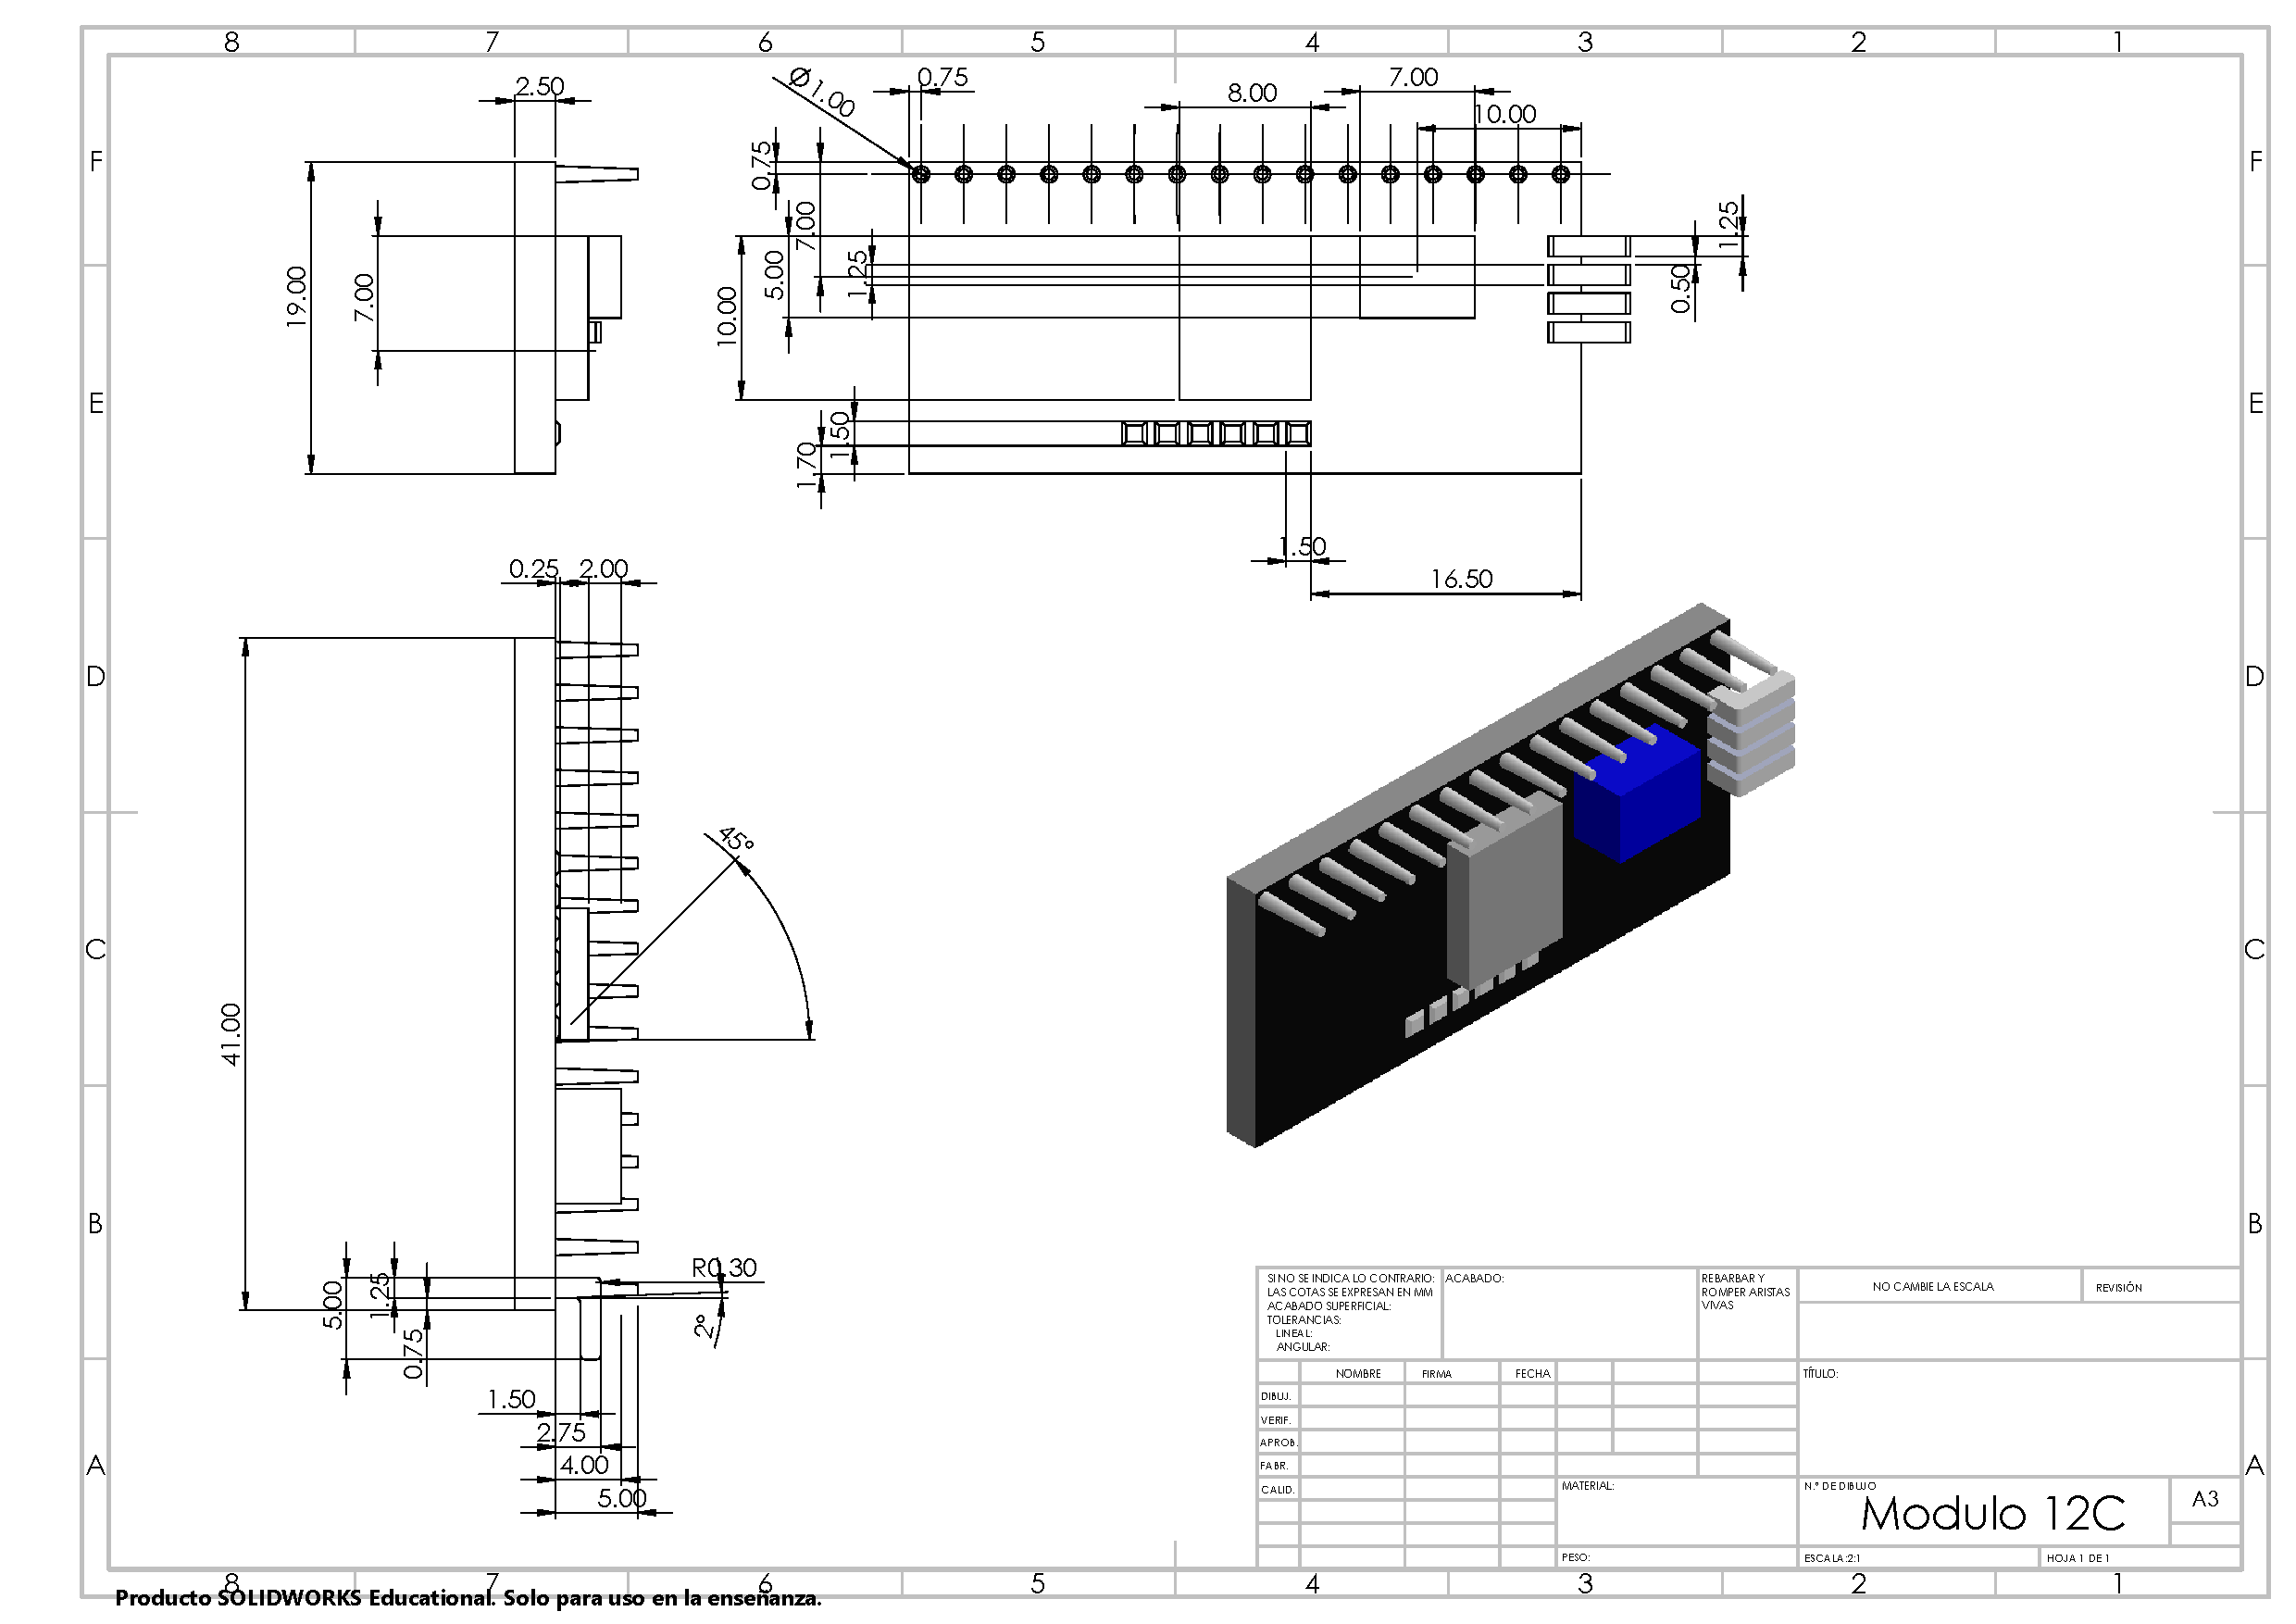
\includegraphics[trim = {10mm 10mm 10mm 10mm},clip,scale=0.150]{16/Img/modulo12C.PDF}
        \caption{Modulo 12C}
       \label{fig:Modulo 12C}
     \end{figure}
    % 
    % 
    % 
    % 
    \begin{figure}[H]
        \centering
        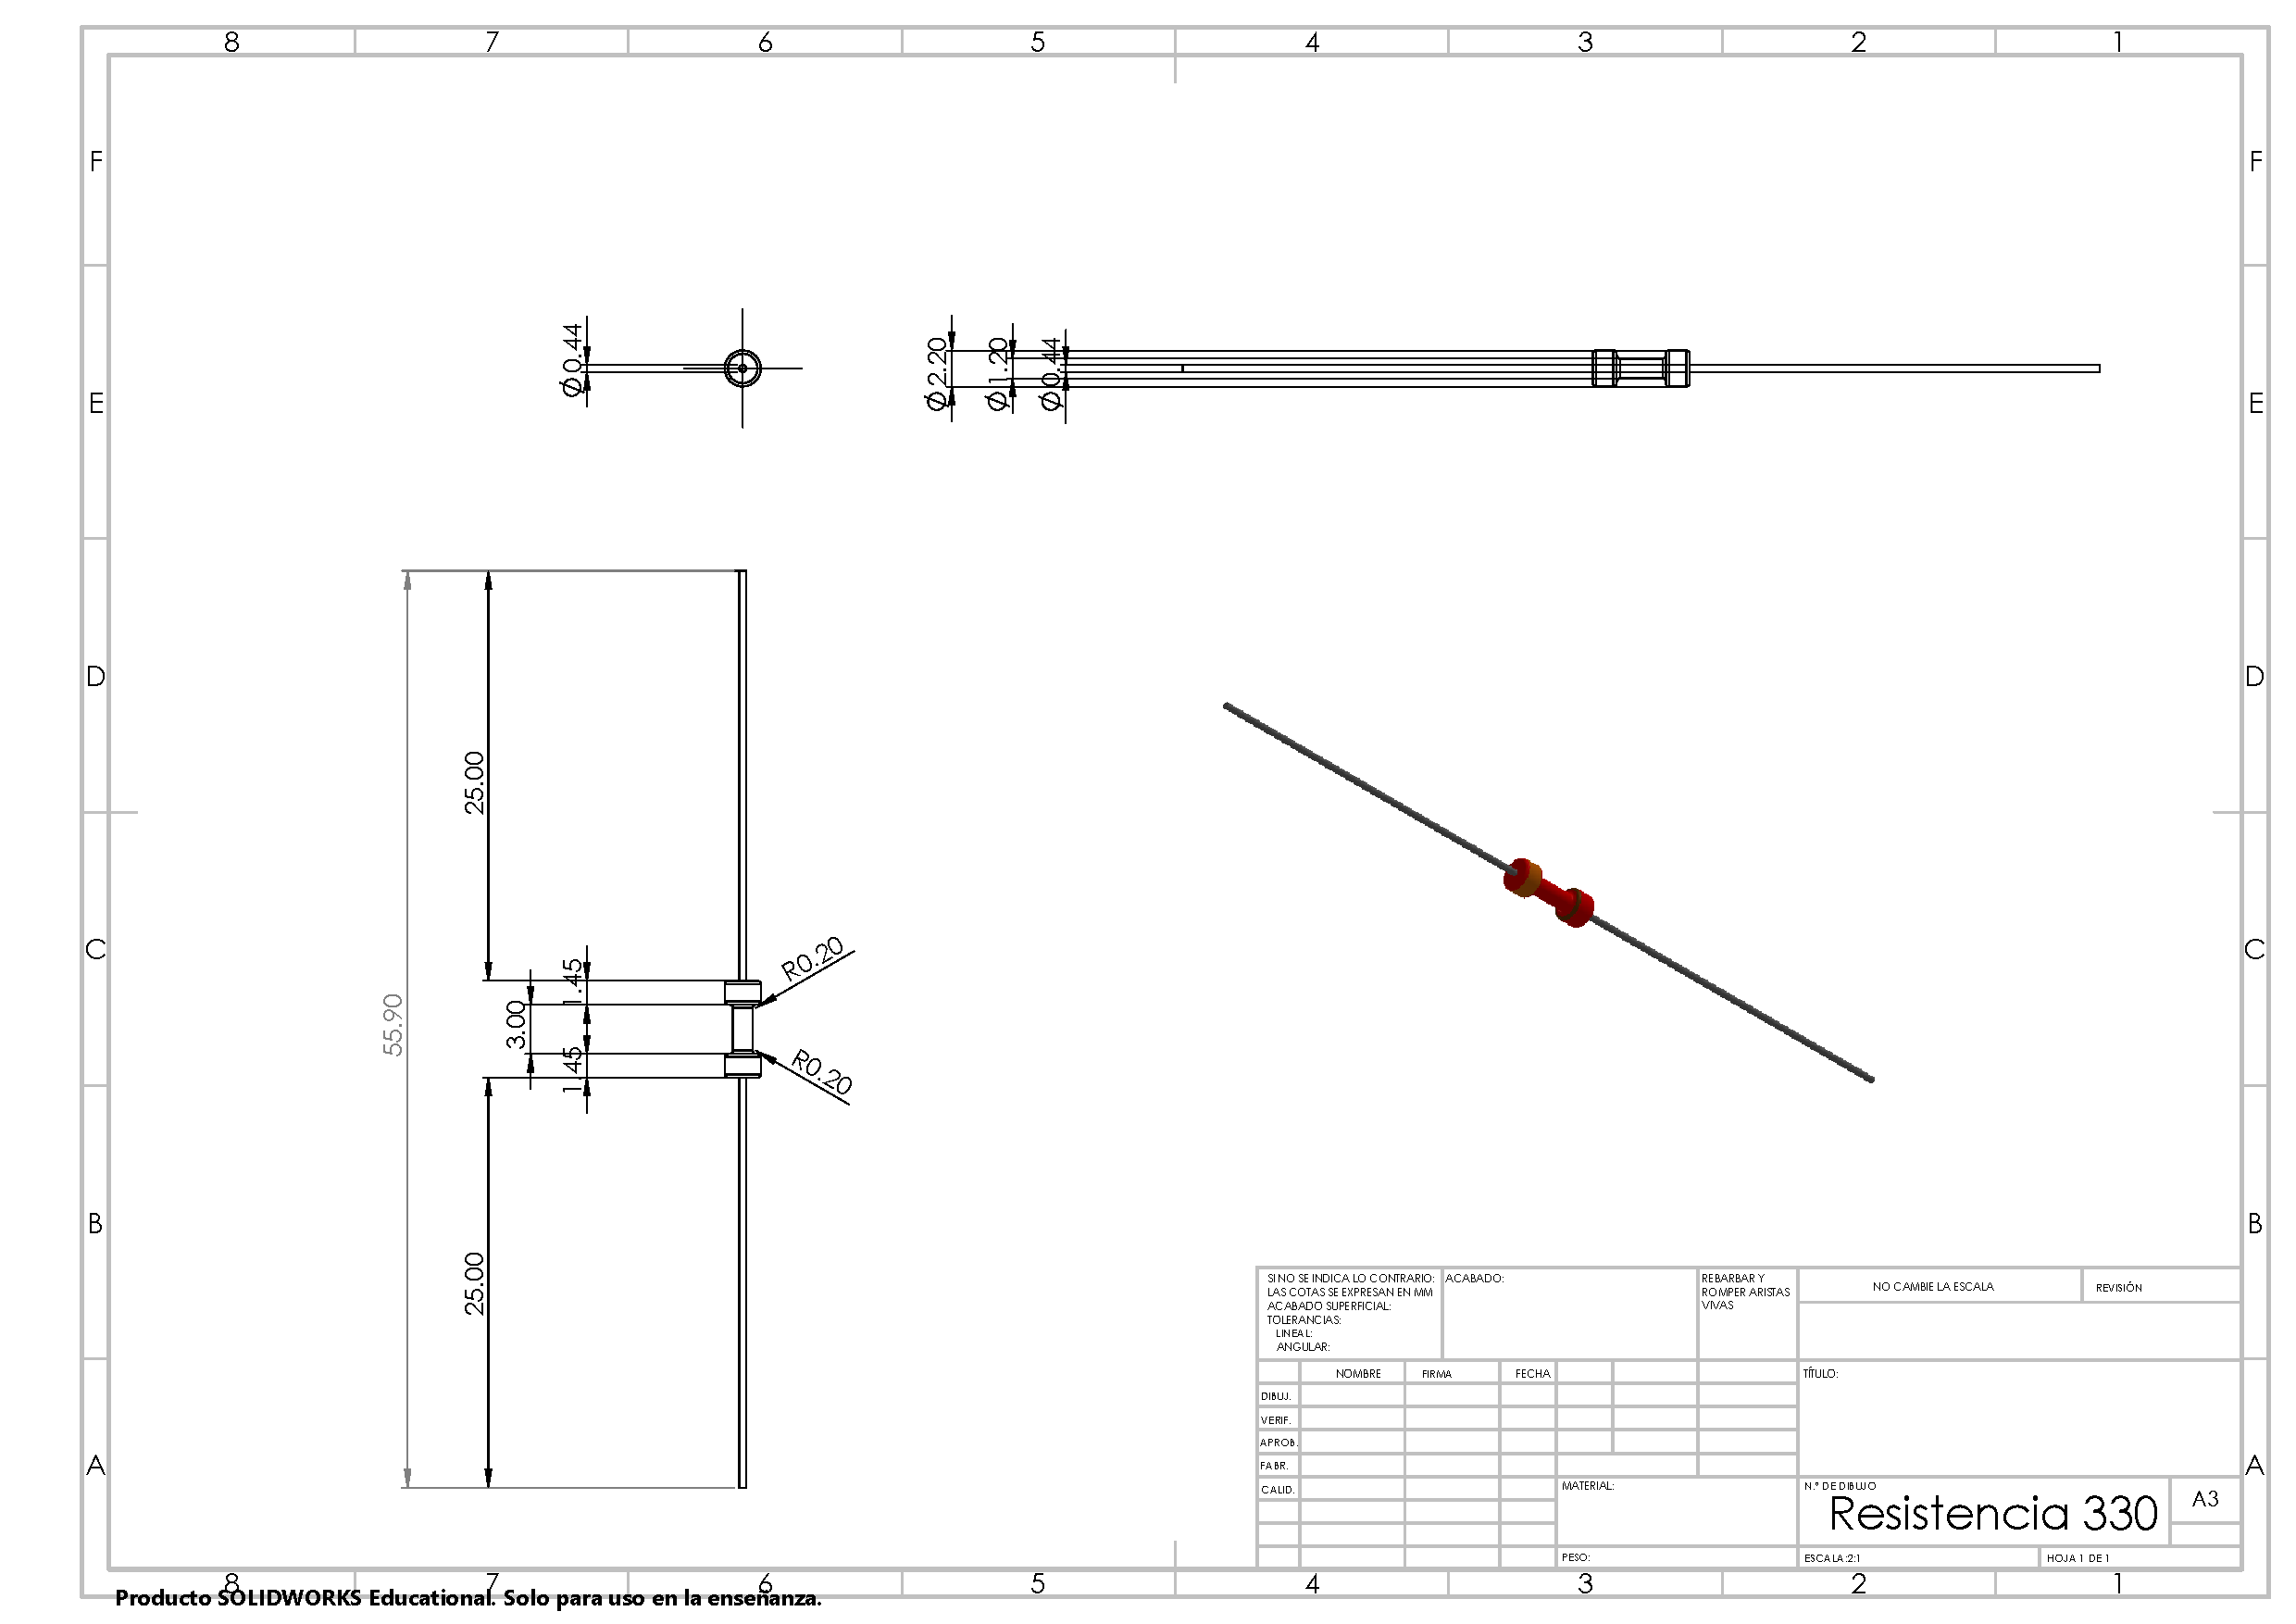
\includegraphics[trim = {10mm 10mm 10mm 10mm},clip,scale=0.150]{16/Img/resistencia330.PDF}
        \caption{Resistencia 330.PDF}
        \label{fig:Resistencia 330.PDF}
    \end{figure}
    % 
    % 
    % 
    % 
    \begin{figure}[H]
        \centering
        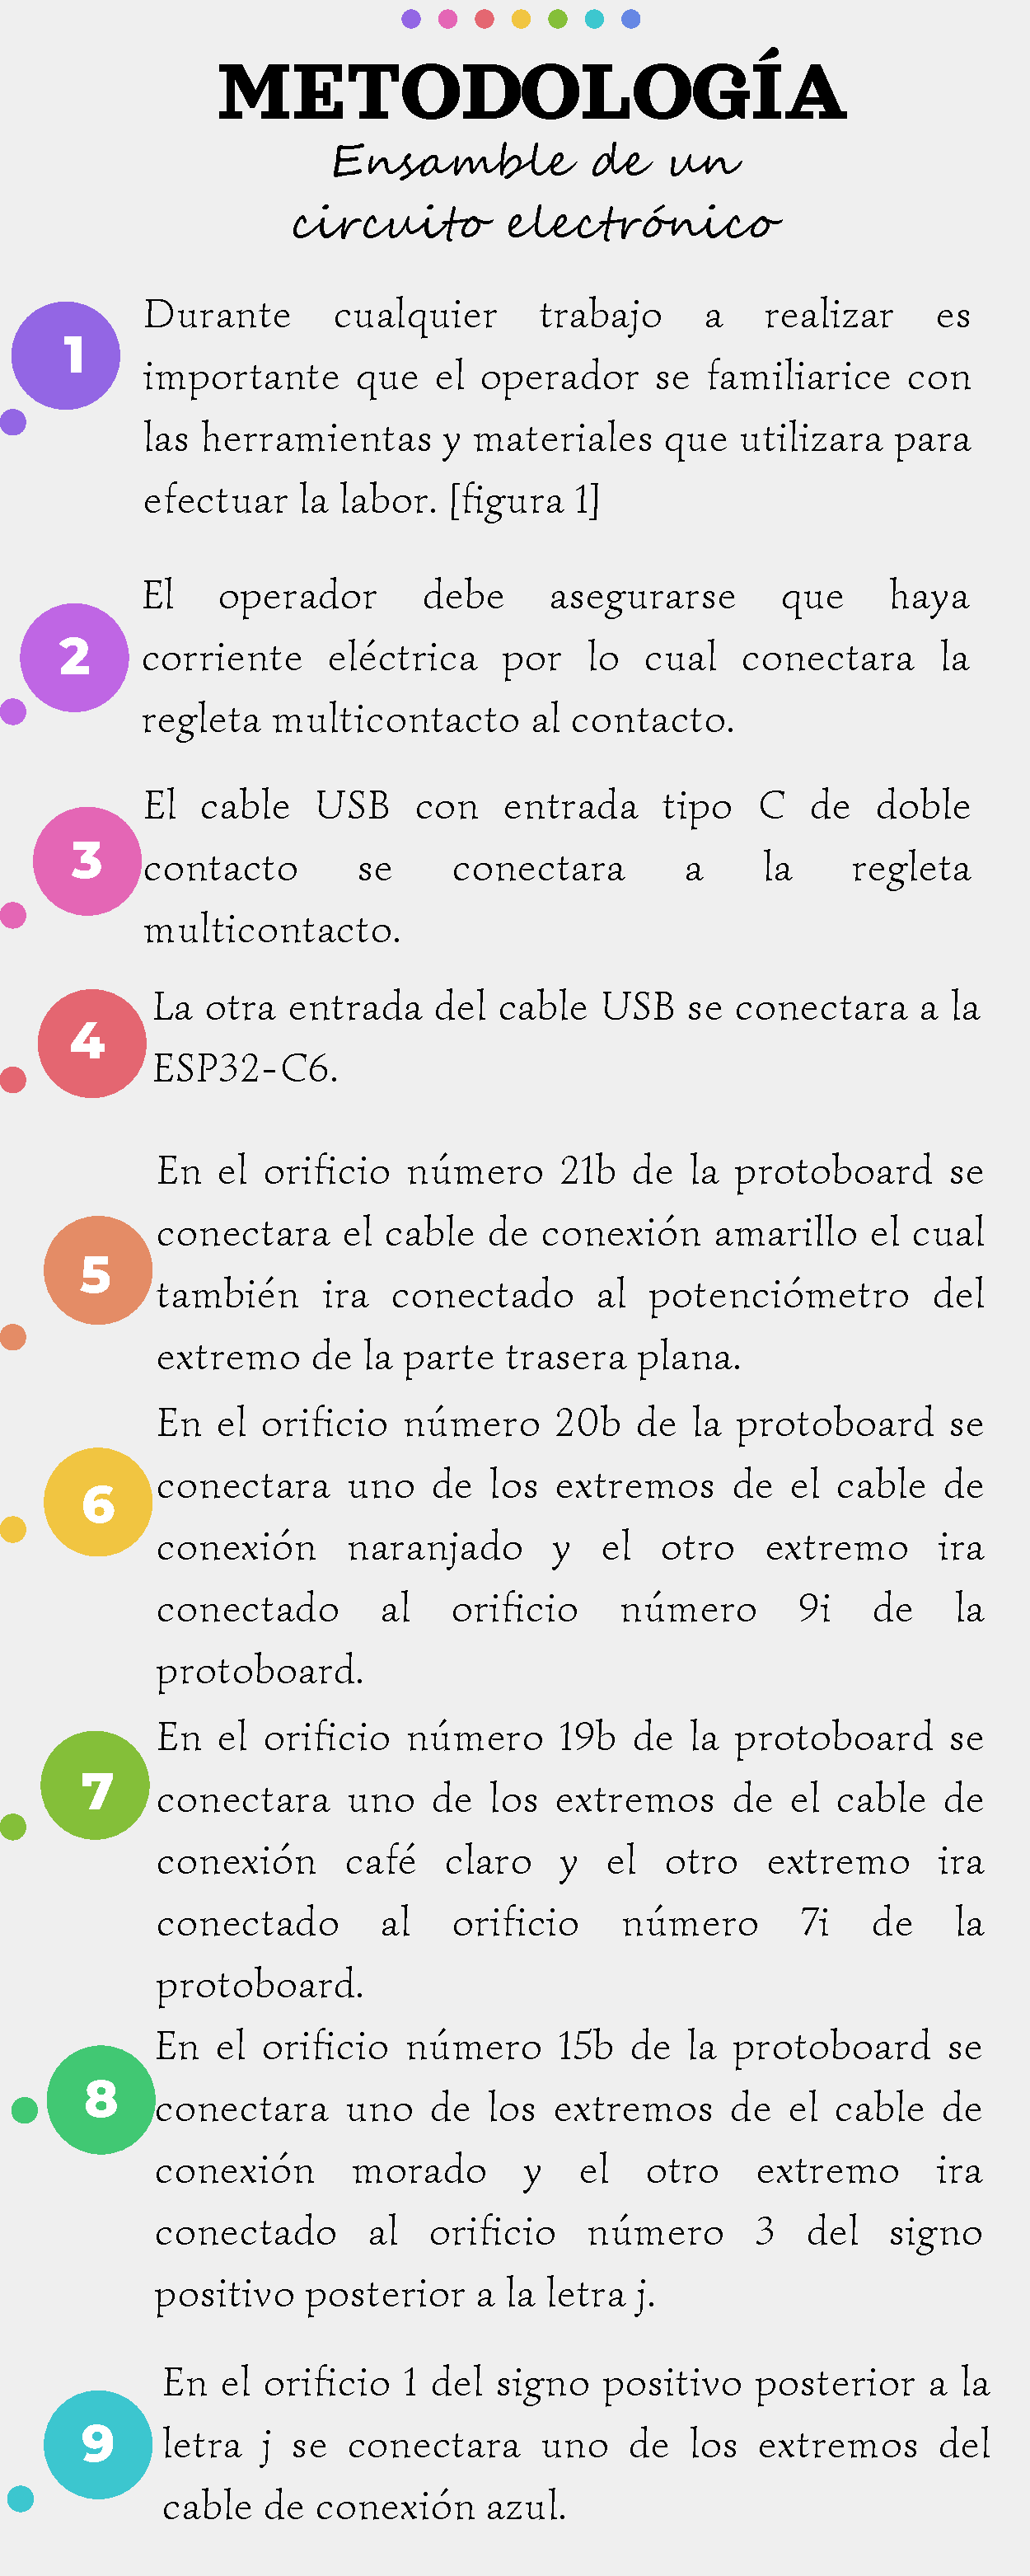
\includegraphics[trim = {5mm 10mm 5mm 50mm},clip,scale=0.4]{16/Img/instructivoCE(1).pdf}
        \caption{Metodología}
        \label{fig:InstructivoCE1)}
    \end{figure}
    % 
    % 
    % 
    % 
    \begin{figure}[H]
        \centering
        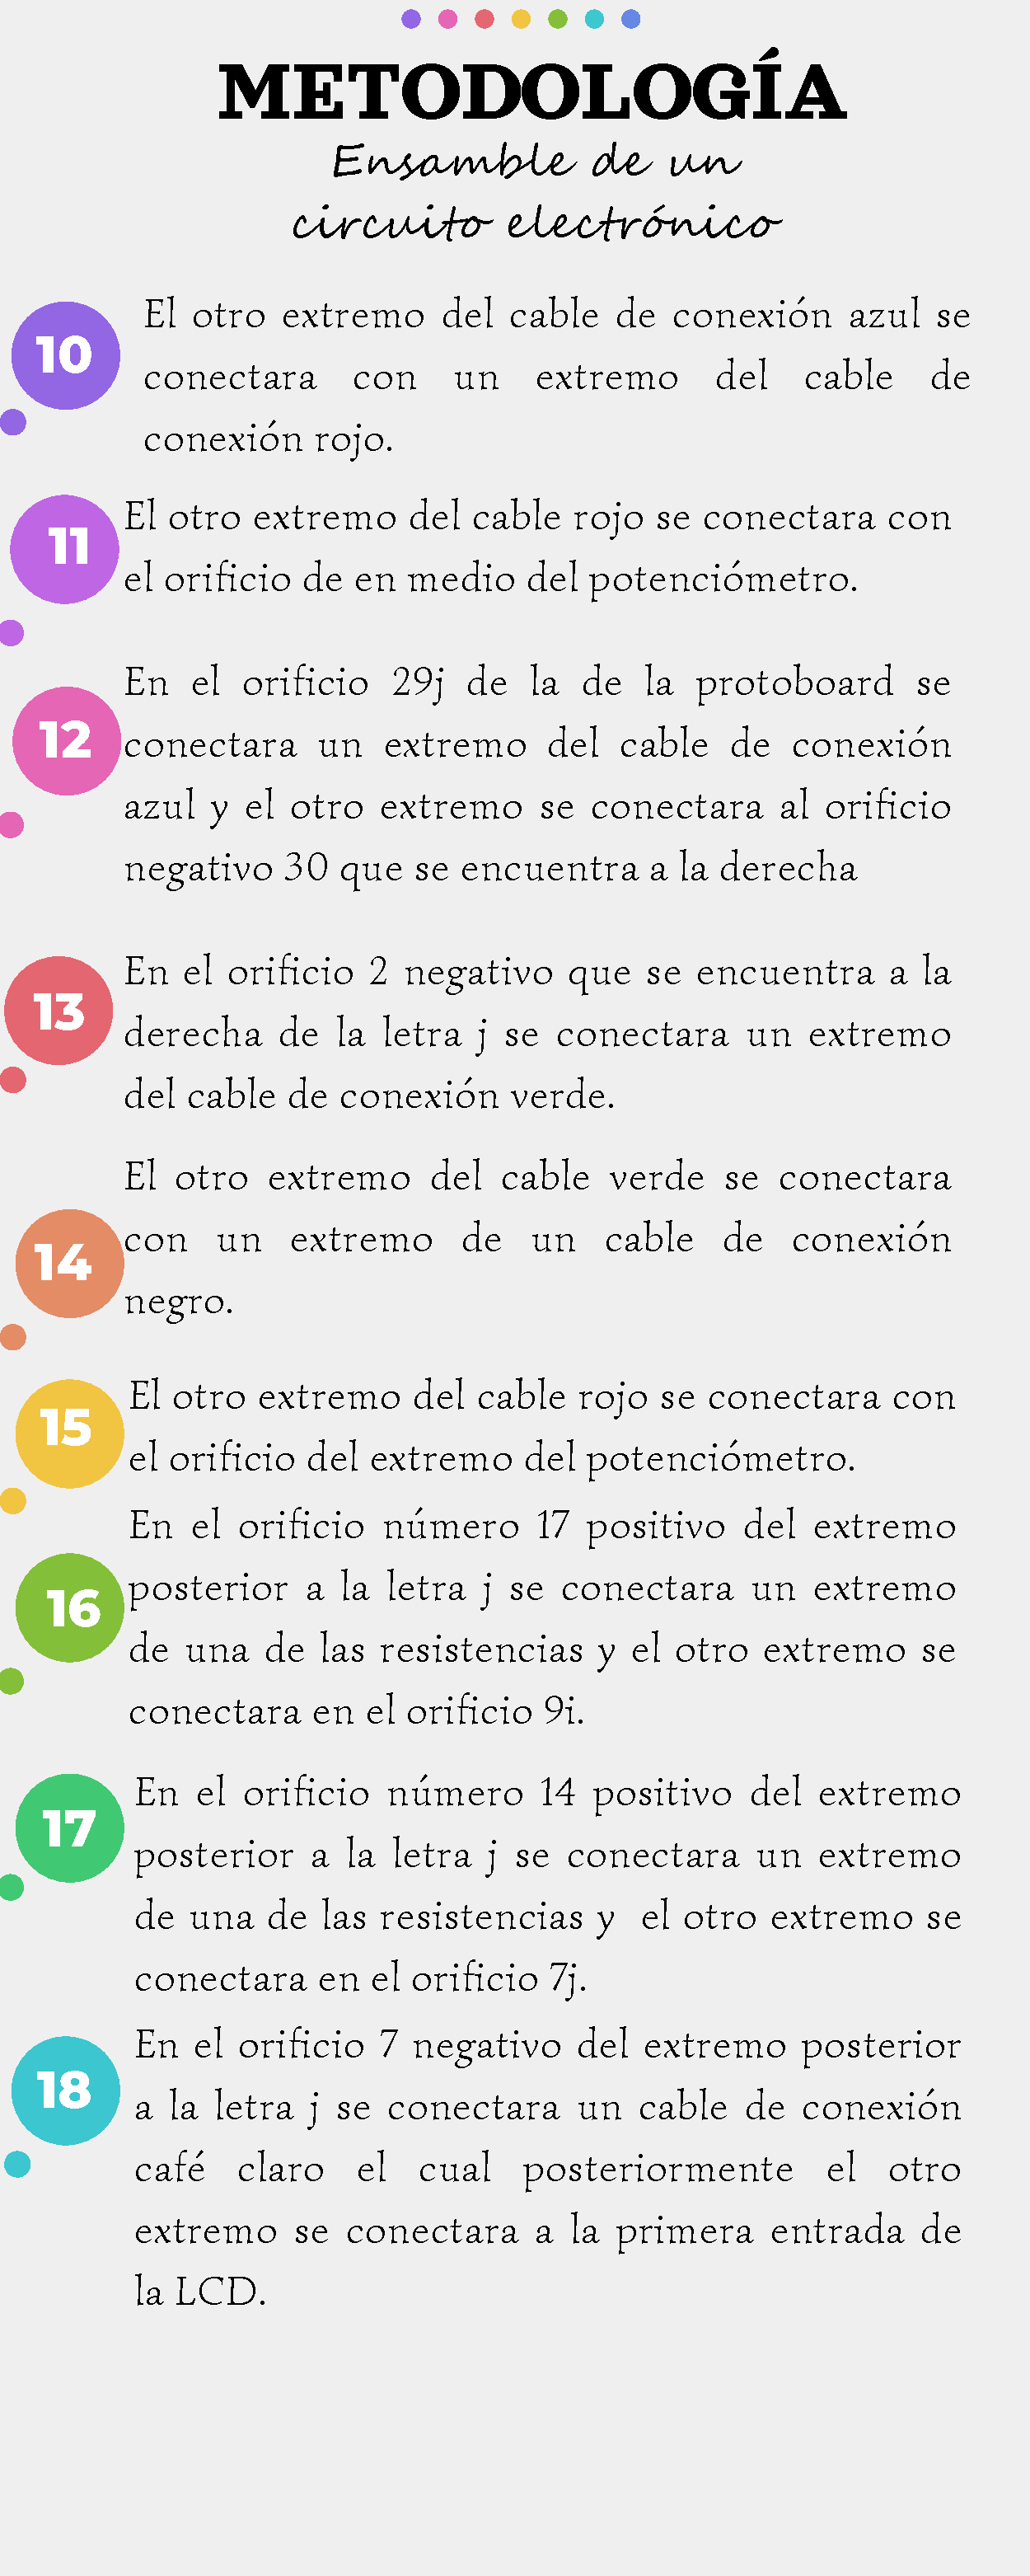
\includegraphics[trim = {5mm 10mm 5mm 50mm},clip,scale=0.4]{16/Img/instructivoCE(2).pdf}
        \caption{Metodología}
        \label{fig:InstructivoCE2}
    \end{figure}
    % 
    % 
    % 
    % 
    \begin{figure}[H]
        \centering
        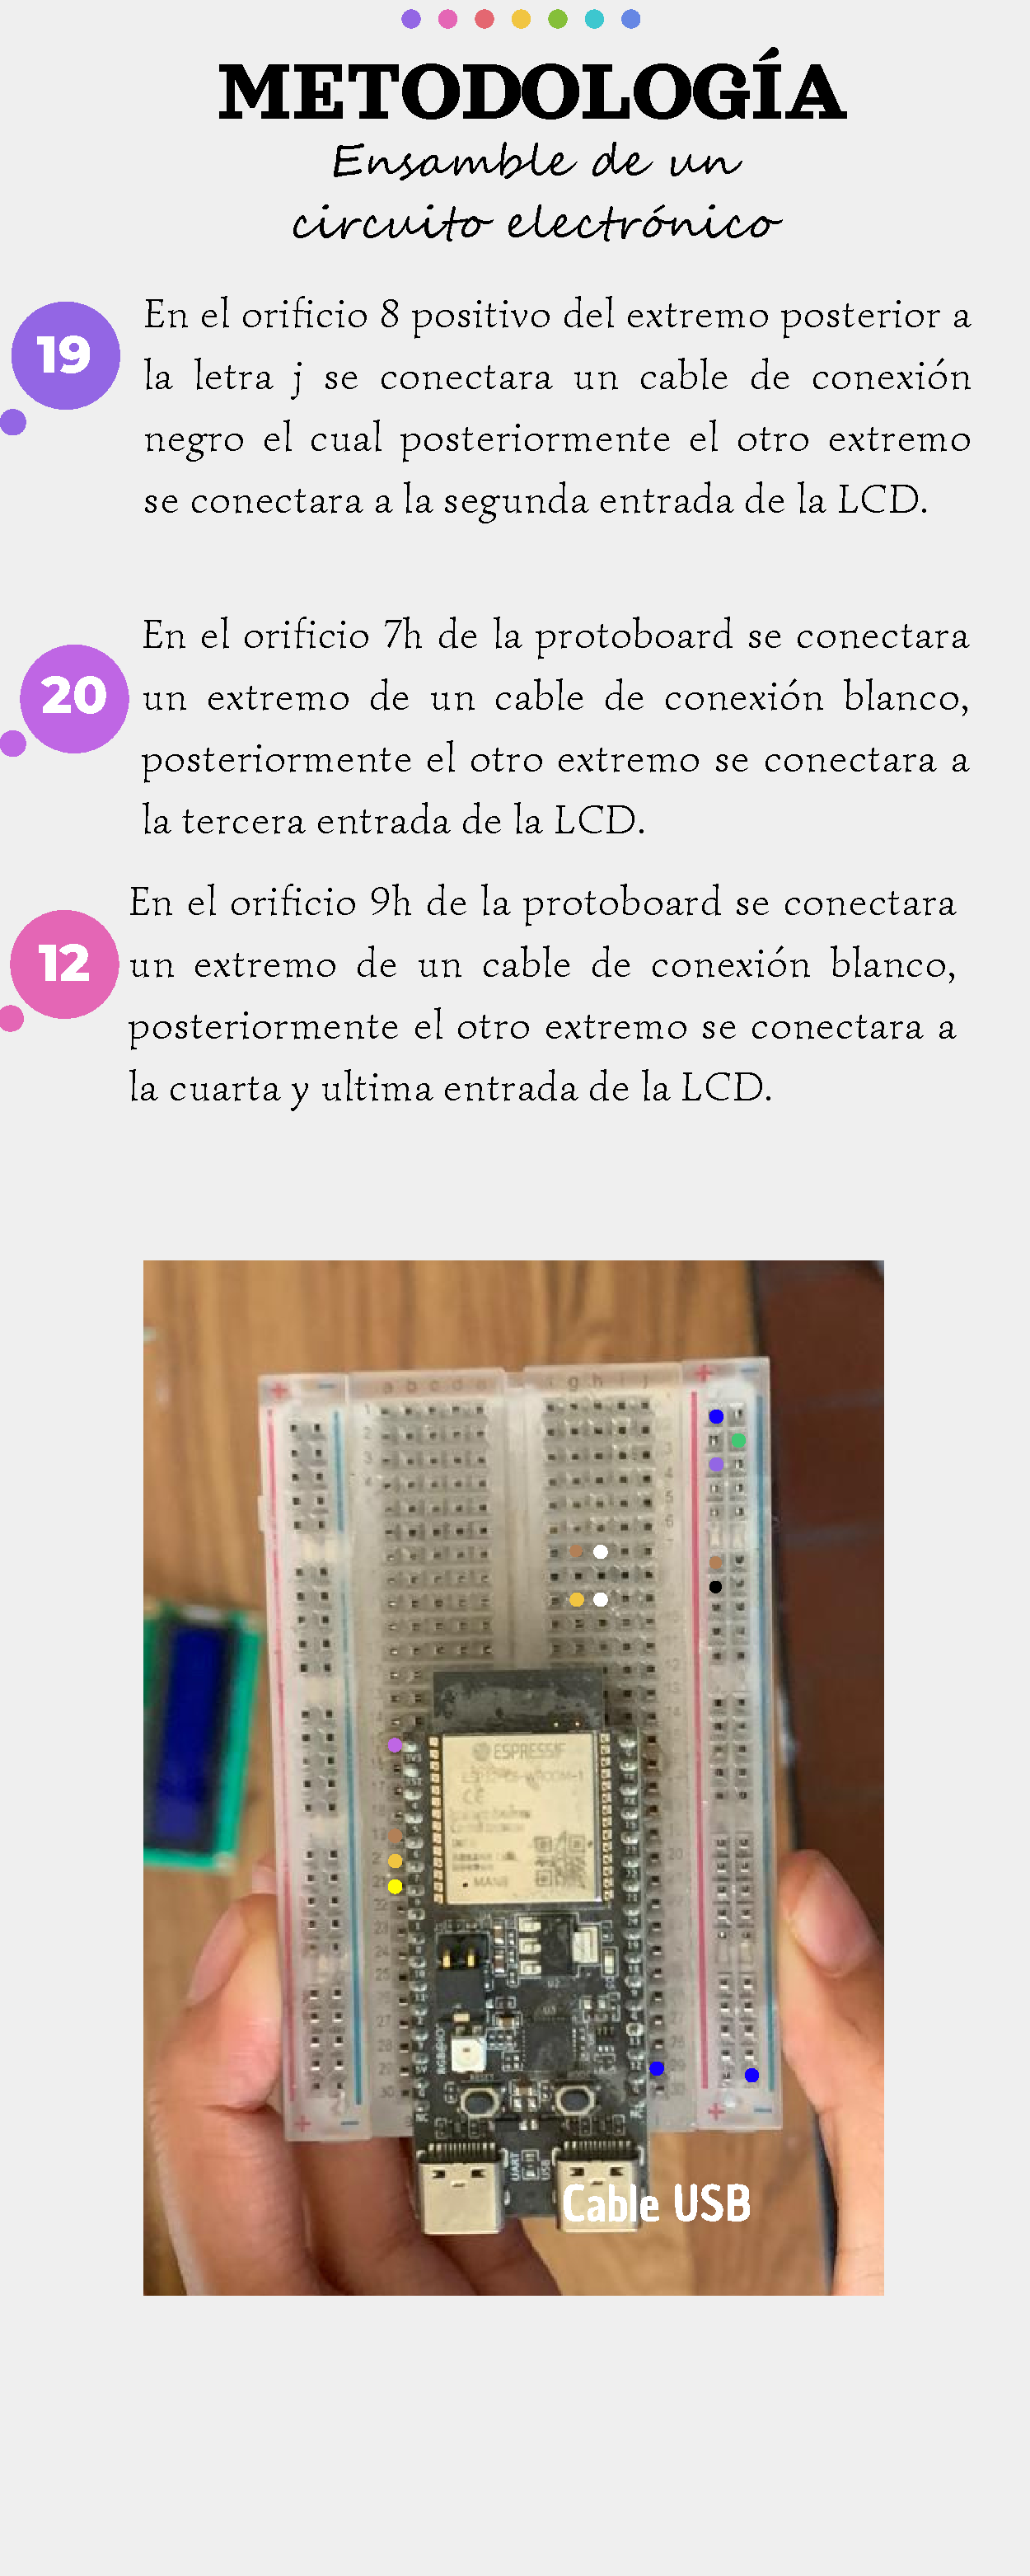
\includegraphics[trim = {5mm 10mm 5mm 50mm},clip,scale=0.4]{16/Img/instructivoCE(3).pdf}
        \caption{Metodología}
        \label{fig:metodología}
    \end{figure}
    % 
    % 
    % 
    % 
    \begin{figure}[H]
        \centering
        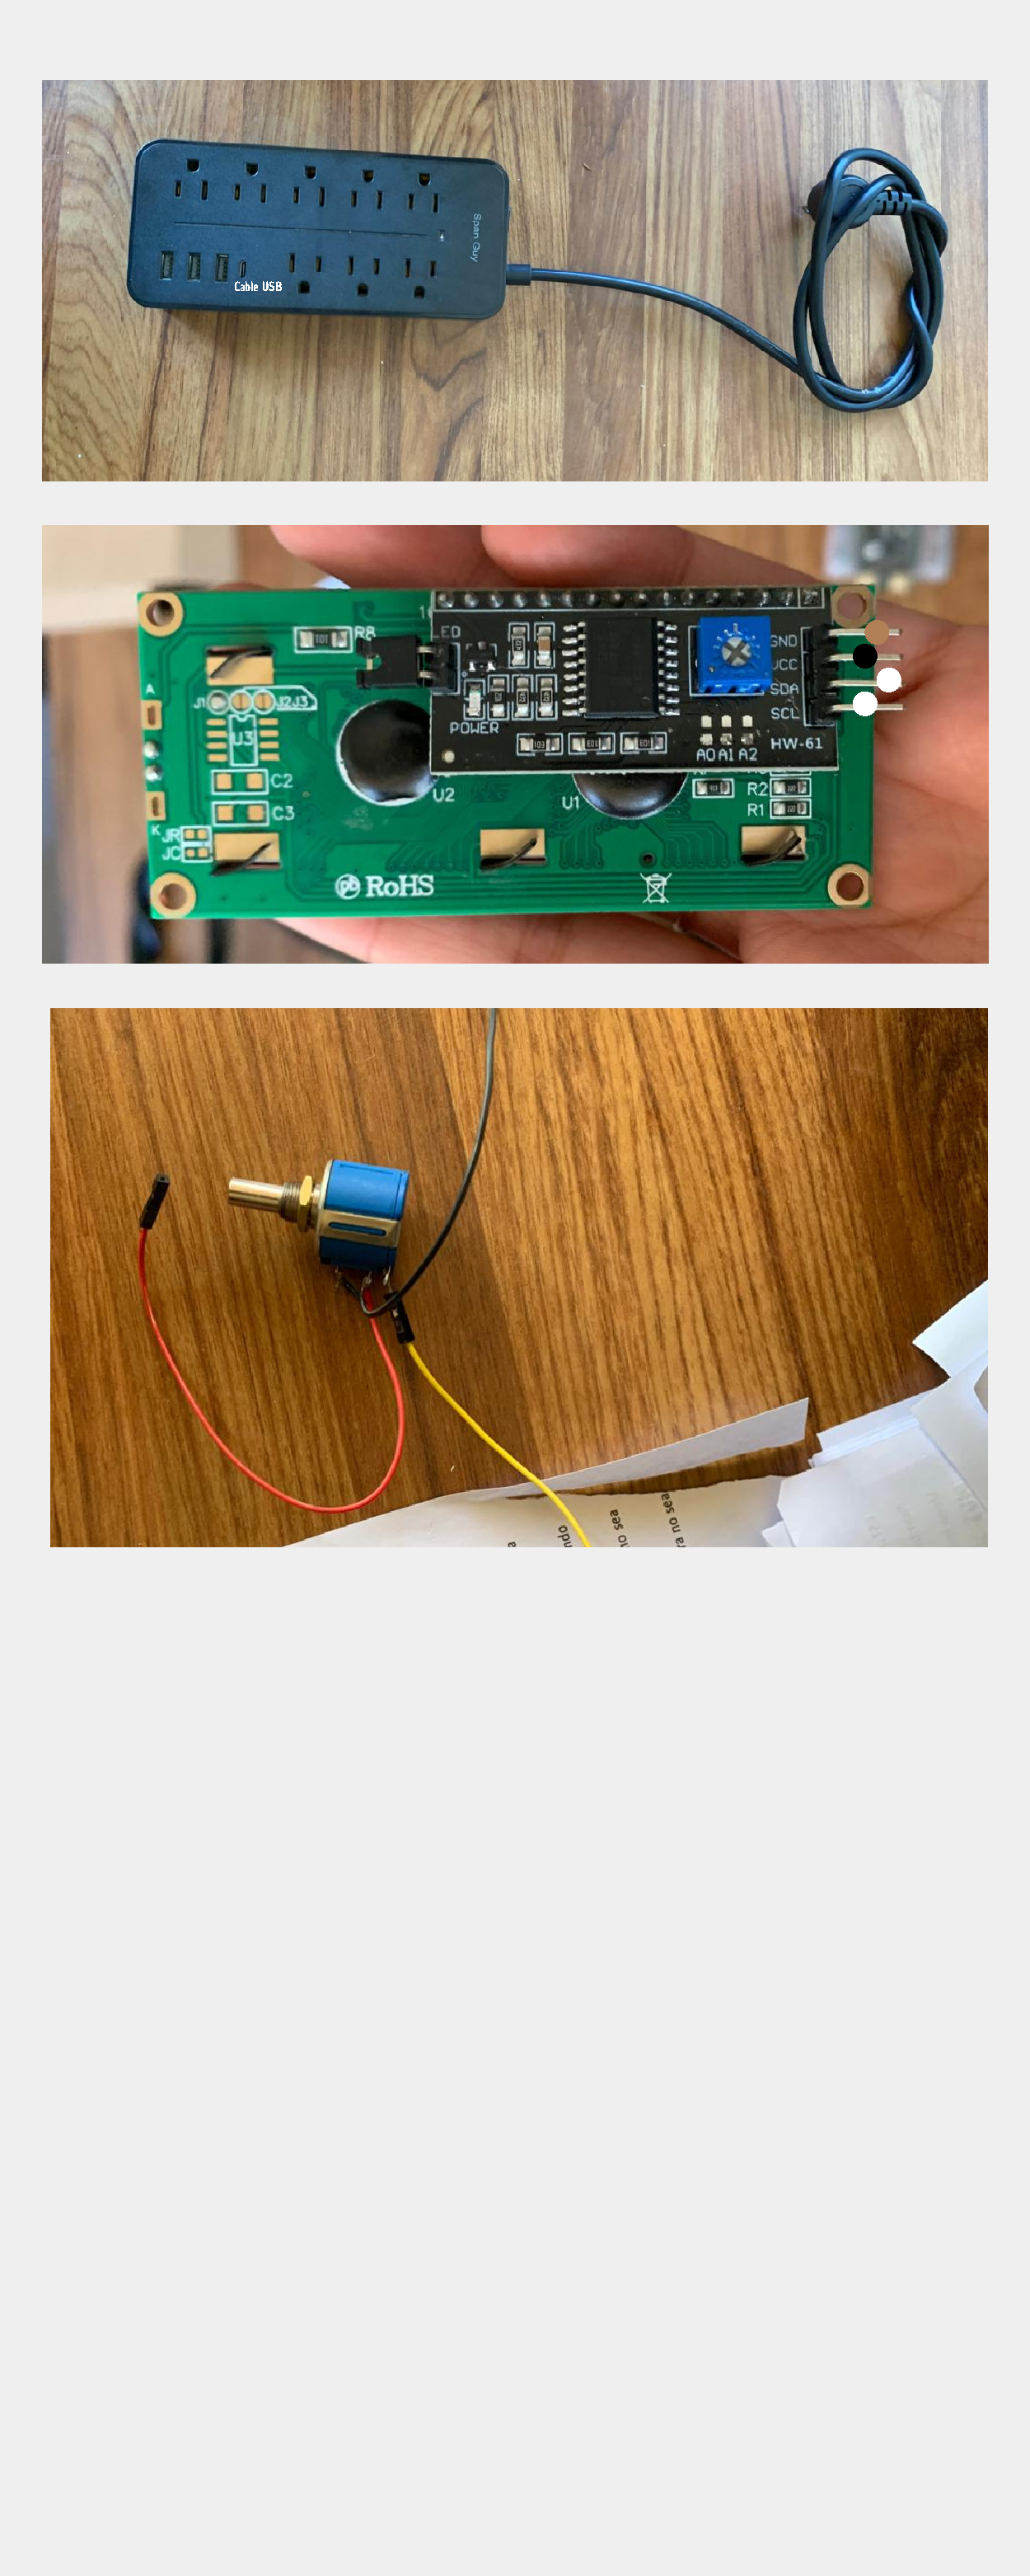
\includegraphics[trim = {5mm 180mm 5mm 30mm},clip,scale=0.4]{16/Img/instructivoCE(4).pdf}
        \caption{Metodología}
        \label{fig:InstructivoCE4}
    \end{figure}
    % 
    % 

    % 
    \subsection{Desarrollo de la guía de plan de Emergencia}
    El Plan de Emergencia: Documento que describe los lineamientos a seguir, la organización y los mecanismos, que indican la manera de enfrentar una situación de emergencia o desastre tanto en lo general como en lo particular, así como la utilización viable de los recursos humanos y materiales con los que se cuenta.
    
    
  
      %\item Se debe establecer que se habrá de hacer, como, conque, y donde para obtener la información que permita probar la hipótesis.  
      %\item Se debe desglosar de acuerdo a los objetivos específicos. 
      %\item Se debe establecer una estrategia metodológica por cada objetivo específico. De manera simplista se podría decir que se cambia el verbo en infinitivo por su respectivo adverbio.
      %\item En cada objetivo se debe describir que método, que materiales y que equipo se usará para conseguirlo.
     % \item Se deben tener referencias Figura \ref{fig:lcd-16x2}.

    % 
    % 
    \begin{figure}[H]
    
    \end{figure}

    %
    % 
\subsection{Análisis de los métodos, materiales, herramientas e instalación utilizada en la ejecución del ensamble de un circuito electrónico}
\subsubsection{Planeación}

\subsubsection{5´s}
Adoptar el método de las 5´s en el ámbito industrial es una táctica efectiva para optimizar la productividad, elevar la calidad, garantizar la seguridad y aumentar la satisfacción de los trabajadores. Al promover una cultura de orden, limpieza y estandarización, las empresas pueden experimentar innovación en su rendimiento operativo y su competitividad.

\subsubsection{Desarrollo del muestreo del trabajo}
El muestreo del trabajo es una técnica importante dentro de la industria para mejorar la eficiencia, reducir costos,lo cual dentro de nuestro proyecto representa la primer etapa del estudio de tiempos y movimientos, también nos ayuda a asegurar la calidad y promover la seguridad. Al proporcionar datos detallados sobre el uso del tiempo y las actividades de los trabajadores, permite tomar decisiones informadas y desarrollar estrategias efectivas para optimizar los procesos laborales.
% 
% 

\subsection{Acrónimos y Abreviaciones}
    
Los acrónimos y abreviaciones deberán ser definidos únicamente la primera vez que aparecen en el texto, esto para que el lector entienda lo que significan.
    
\subsection{Ecuaciones}
    
Las ecuaciones son una excepción a las especificaciones prescritas de esta plantilla. 
Deberá determinar si su ecuación debe escribirse o no utilizando la fuente Adobe Devangari. 
Para crear ecuaciones multinivel, puede ser necesario tratar la ecuación como un gráfico e insertarla en el texto después de aplicar el estilo de la platilla.
Las ecuaciones serán enumeradas de manera consecutiva, y el número de ecuación, entre paréntesis, se colocan al ras de la derecha, utilizando una tabulación derecha. 
    
    \begin{equation}
        \label{eq1}
        x + y = z 
    \end{equation}
    
    Es importante asegurarse de que los símbolos de la ecuación sean definidos antes o inmediatamente después de la ecuación. Utilice “(1)”, en vez de “Eq. 1” al enumerar las ecuaciones, excepto al principio de una oración: “La ecuación (\ref{eq1}) es…”
    
    \section{Resultados y discusión}
    \subsection{Desarrollo de la guía de plan de Emergencia}
    
El Plan de Emergencia: Documento que describe los lineamientos a seguir, la organización y los mecanismos, que indican la manera de enfrentar una situación de emergencia o desastre tanto en lo general como en lo particular, así como la utilización viable de los recursos humanos y materiales con los que se cuenta.Así como su objetivo es implementar las estrategias para proporcionar seguridad a las personas, sus bienes y todo lo que lo rodea mediante procedimientos antes, durante y después de una situación de emergencia.\ref{fig:Plano de localización ITQ}
\begin{figure}[H]
    \centering
    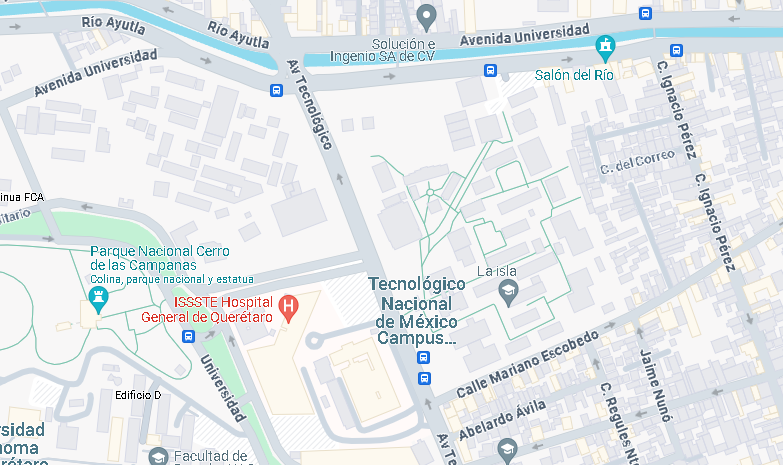
\includegraphics[scale=0.4]{16/Img/mapaitq.PNG}
    \caption{ Plano de localización del Tecnológico Nacional de México, Av. Tecnológico s/n esq. Gral. Mariano Escobedo, Centro Histórico, 76000, Santiago de Querétaro, QRO, México, +52 442 216 3597/(442) 227 44 00}
    \label{fig:Plano de localización ITQ}
\end{figure}
    %
    %
    %Antes de comenzar a preparar tu artículo, es importante que lea primero la guía del autor, la cual incluye los temas o apartados que son necesarios para tener tu trabajo completo.
    %Una vez completada la edición del texto, el documento está listo para el uso de esta plantilla. En este archivo recién creado, resalte todo el contenido e importe el archivo de texto preparado. Ahora esta listo para estilizar su documento.
    %En esta sección se deben presentar todo lo obtenido de la sección 2, incluidas deducciones o efectos del desarrollo. También se podrán incluir subsecciones numeradas de la siguiente forma:
    
    \subsubsection{Identificación del riesgo}
    
    Estamos dedicados a mantener diariamente un programa interno de prevención de riesgos. Asimismo, apreciamos la retroalimentación de clientes internos y externos sobre los peligros que surgen o pueden surgir durante las actividades cotidianas dentro de nuestras instalaciones. Por ello, les animamos a utilizar el equipo de trabajo adecuado, recordando así la importancia que conlleva usar 
    adecuadamente nuestro EPP. Evaluamos cada riesgo interno utilizando una clasificación para dar prioridad a las acciones que nos generan mayor riesgo para nuestro personal, garantizando así una gestión eficaz de los peligros identificados.\ref{Riesgos}
    %
    %
    \begin{figure}[H]
        \centering
        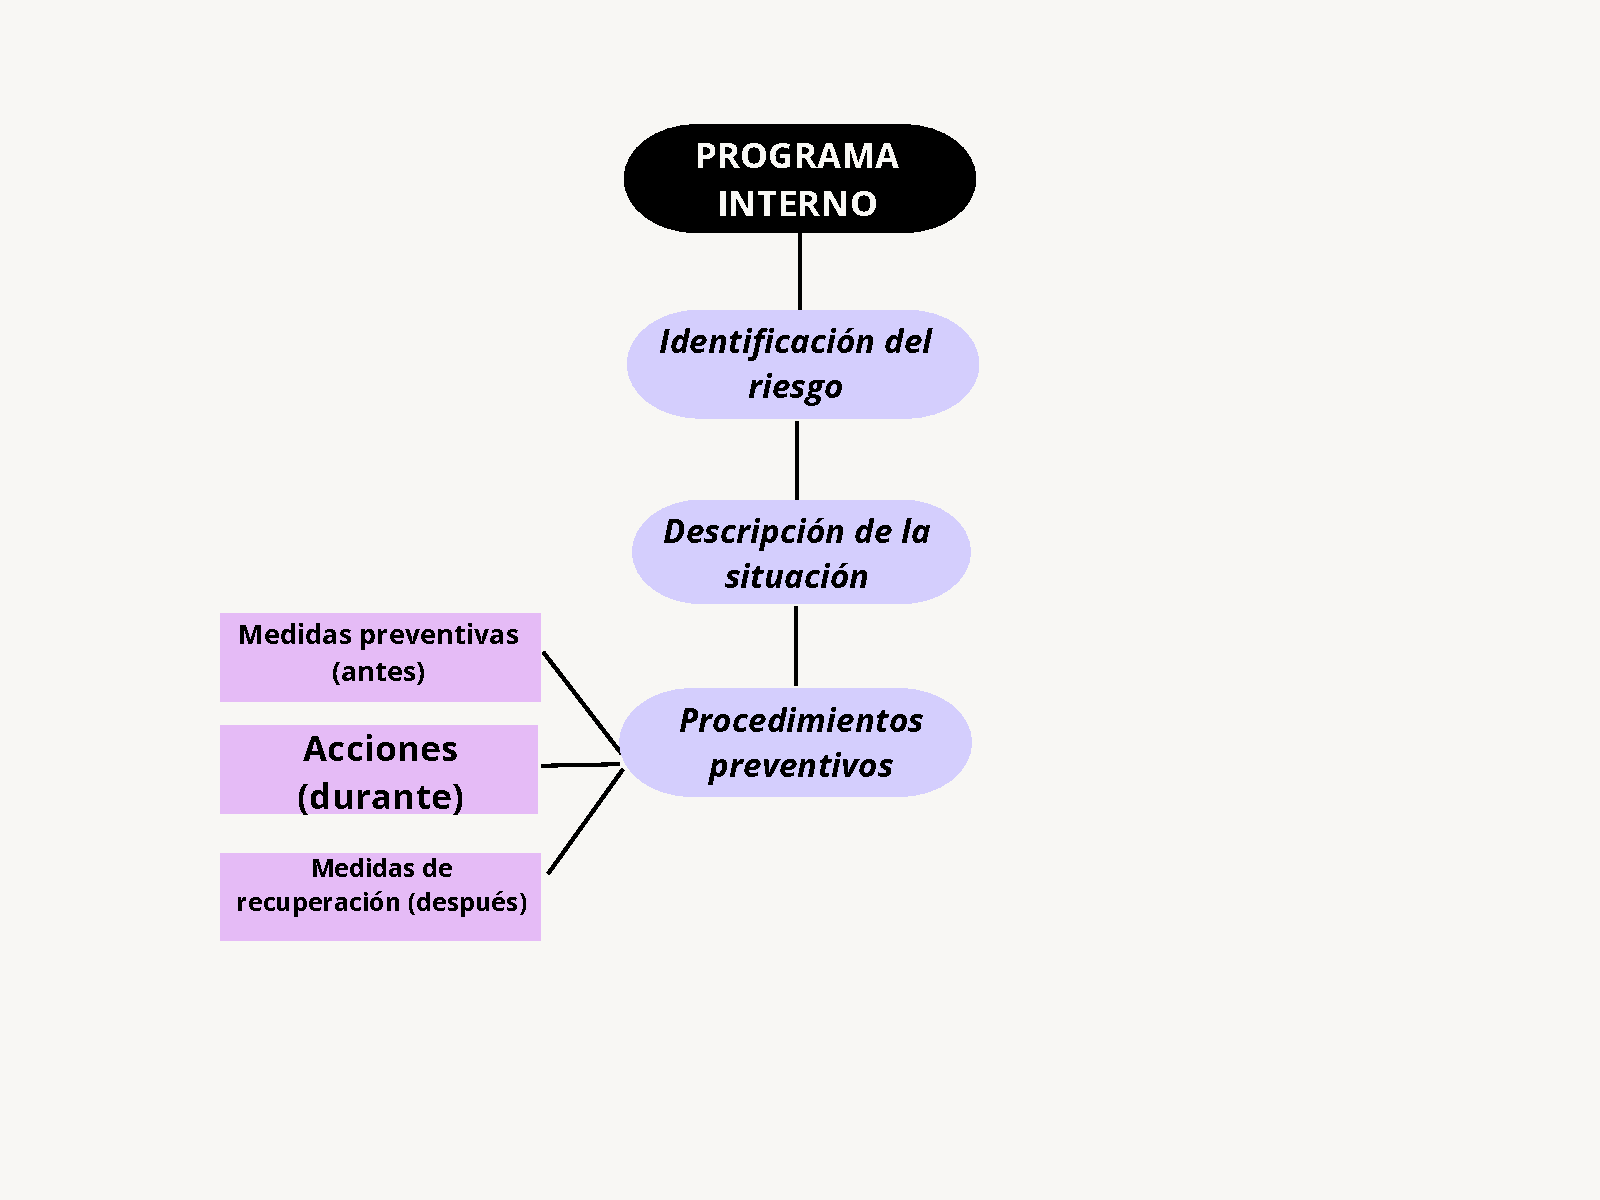
\includegraphics[trim = {25mm 25mm 32mm 20mm},clip,scale=0.40]{16/Img/programainterno.pdf}
        \caption{Riesgos}
        \label{Riesgos}
    \end{figure}
    
    \subsubsection{Riesgos internos}
   Definimos el riesgo como la posibilidad de que se produzca un evento no deseado o perjudicial en algún sentido. Con esto vamos a evaluar la posibilidad de que la institución se enfrente a problemas originados por fallos internos en su funcionamiento cotidiano. Con esto podríamos decir que el riesgo implica evaluar un posible daño ante una situación peligrosa, que puede tener consecuencias indeseables.
    \begin{table}[h]
    \centering
    \caption{Riesgos con diferentes niveles y colores para distinguir la gravedad y acciones}
    \begin{tabular}{c c c}
    \hline
    \multicolumn{3}{c}{Riesgos}\\
    \hline
         Alto& 4 - 5 & Rojo  \\
    \hline
         Medio& 3 - 2 & Amarillo  \\
    \hline
         Bajo& 1 - 0 & Verde \\
    \hline     
    \end{tabular}
    \label{tab:riego}
\end{table}
%
%
\begin{figure}[H]
        \centering
        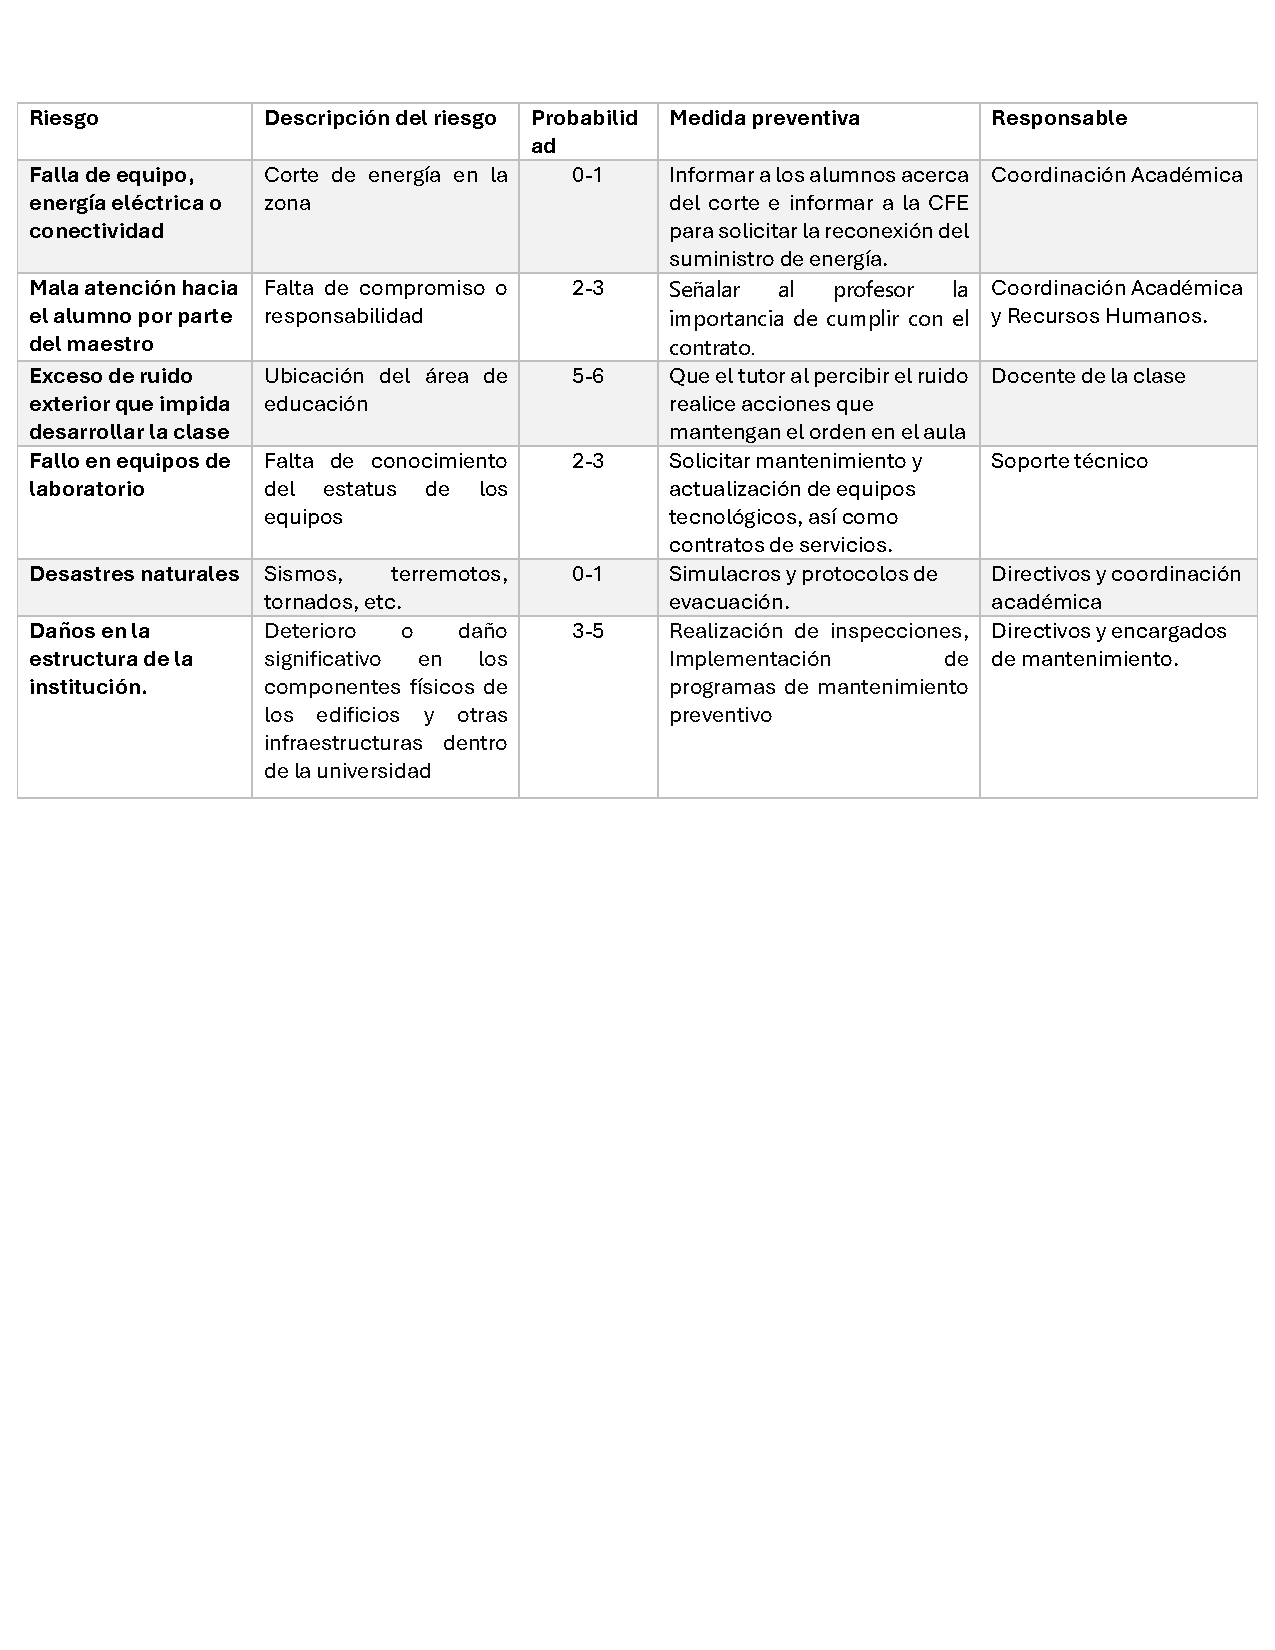
\includegraphics[trim = {5mm 5mm 5mm 15mm},clip,scale=0.42]{16/Img/riesgosinternosITQ.pdf}
        \caption{Riesgos internos}
        \label{Riesgos internos}
    \end{figure}
%
%
\subsubsection{Riesgos externos}
%
%
\begin{figure}[H]
        \centering
        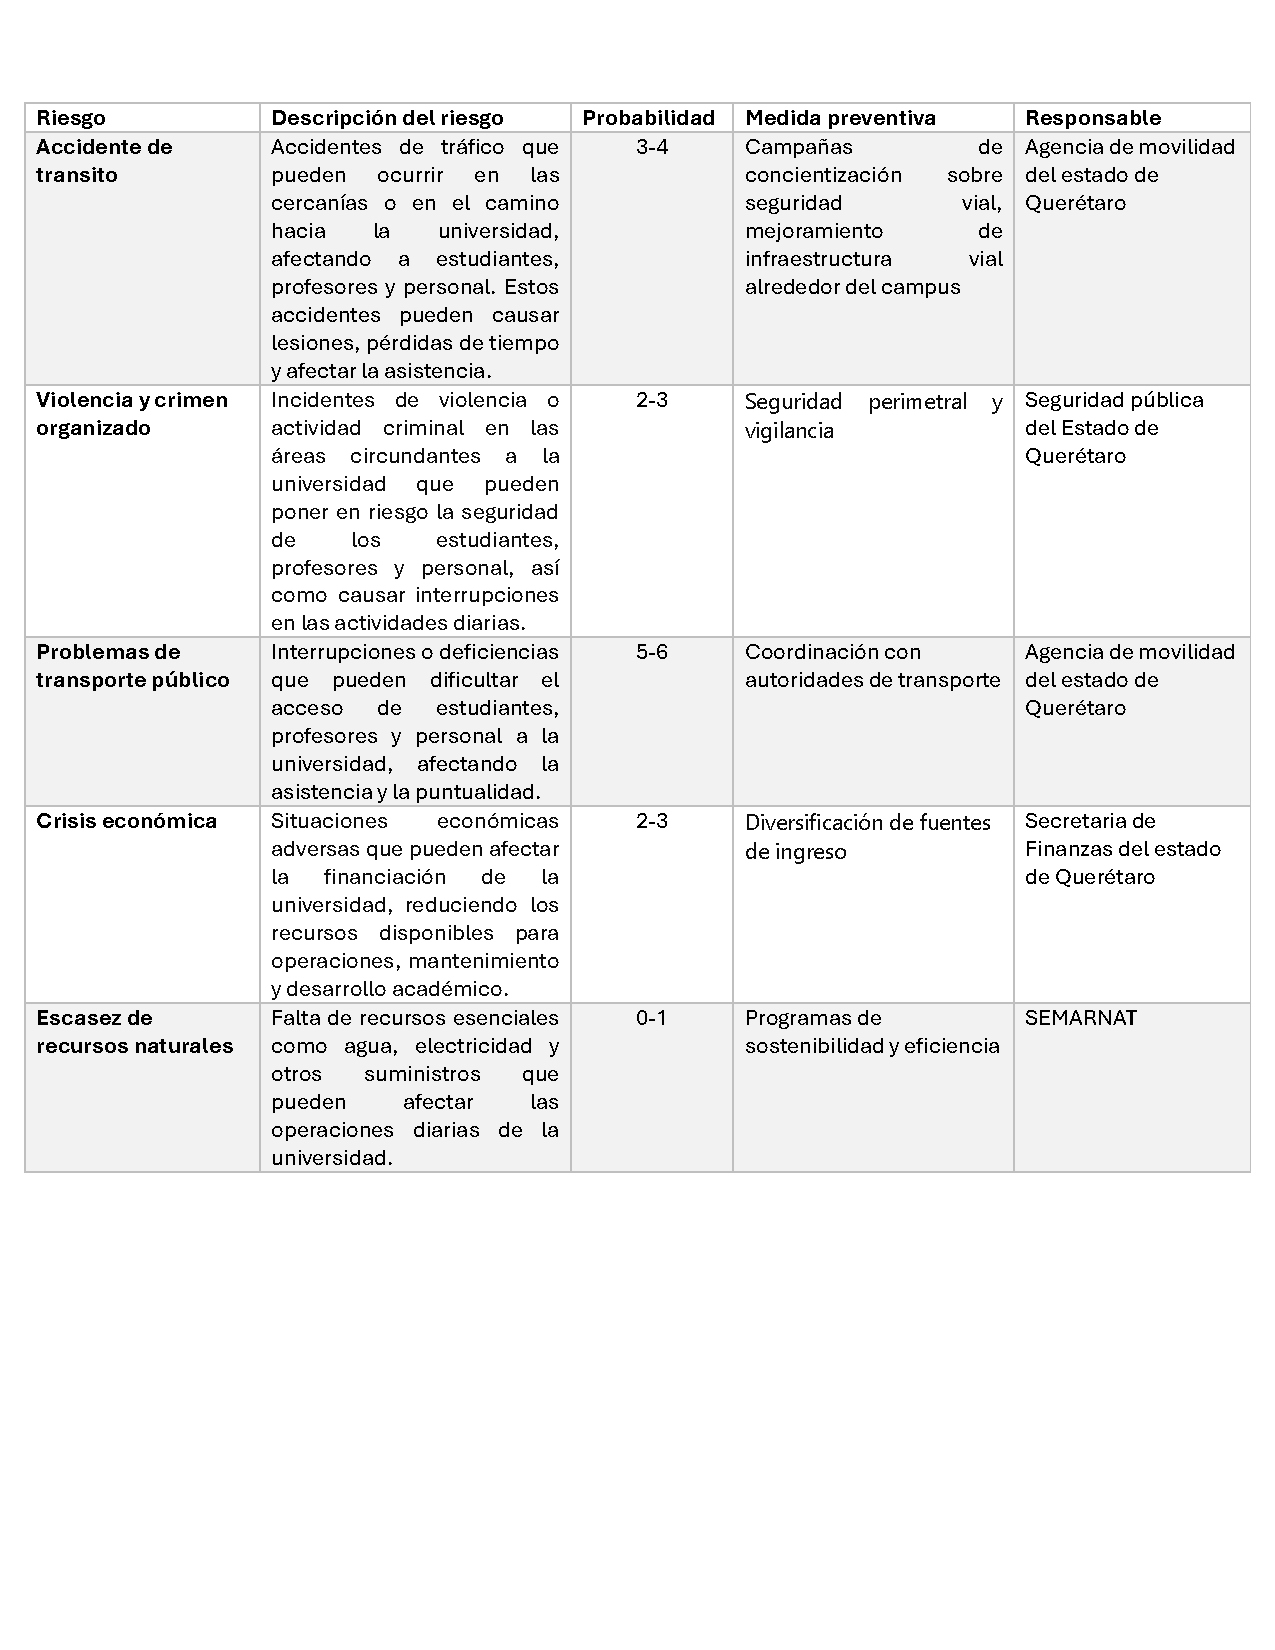
\includegraphics[trim = {5mm 5mm 5mm 15mm},clip,scale=0.42]{16/Img/riesgosexternosITQ.pdf}
        \caption{Riesgos externos}
        \label{Riesgos externos}
    \end{figure}
%
%
\subsubsection{Programa de actividades de prevención y auxilio}
Un Programa de Actividades de Prevención y Auxilio es un plan estructurado diseñado para anticipar, prevenir, y responder de manera efectiva a situaciones de riesgo que puedan afectar a una organización o comunidad. Es importante tener un programa de auxilio en cualquier institución para asegurar la seguridad y el bienestar de las personas, así como la continuidad de las operaciones en caso de emergencias o desastres.Entonces como tal serian las medidas de prevención que se realizan antes de que ocurra en incidente.
\subsubsection{Plan de acción}
Un plan de acción es un conjunto específico de instrucciones que permite al ITQ (Instituto Tecnológico de Querétaro) realizar diferentes tareas y funciones. Estas tareas incluyen la resolución de problemas y la gestión de riesgos tanto internos como externos. El plan detalla los pasos a seguir para identificar y prevenir posibles riesgos, así como las medidas de auxilio a tomar en caso de que ocurra un incidente.

El objetivo del plan de acción es asegurar que todos en la institución sepan qué hacer para mantener la seguridad y la continuidad de las operaciones. Esto incluye la asignación de responsabilidades, la identificación de recursos necesarios, la definición de plazos y la implementación de estrategias de seguimiento y evaluación. En resumen, el plan de acción proporciona una guía clara y detallada para gestionar eficazmente los riesgos y responder a situaciones de emergencia en el ITQ.
%
%
\begin{figure}[H]
        \centering
        \includegraphics[trim = {5mm 5mm 5mm 10mm},clip,scale=0.40]{16/Img/plandeacción.pdf}
        \caption{Plan de acción}
        \label{Plan de acción}
    \end{figure}
%
%
\subsubsection{Identificación de capacidades}

\begin{table}[H]
    \centering
    \caption{Recursos en materia de seguridad}
    \begin{tabular}{c c c}
    \hline
    \multicolumn{3}{c}{Inventario de recursos en materia de seguridad}\\
    \hline
         No.& Recurso & Cantidad  \\
    \hline
         1& Extintor &  3 \\
    \hline
         2& Botiquín & 3 \\
    \hline
         3& Detector de humo & 0 \\
    \hline     
    \end{tabular}
    \label{tab:inventario}
\end{table}
% 
% 
\subsubsection{Plano de localización de recursos}
%
%
\begin{figure}[H]
        \centering
        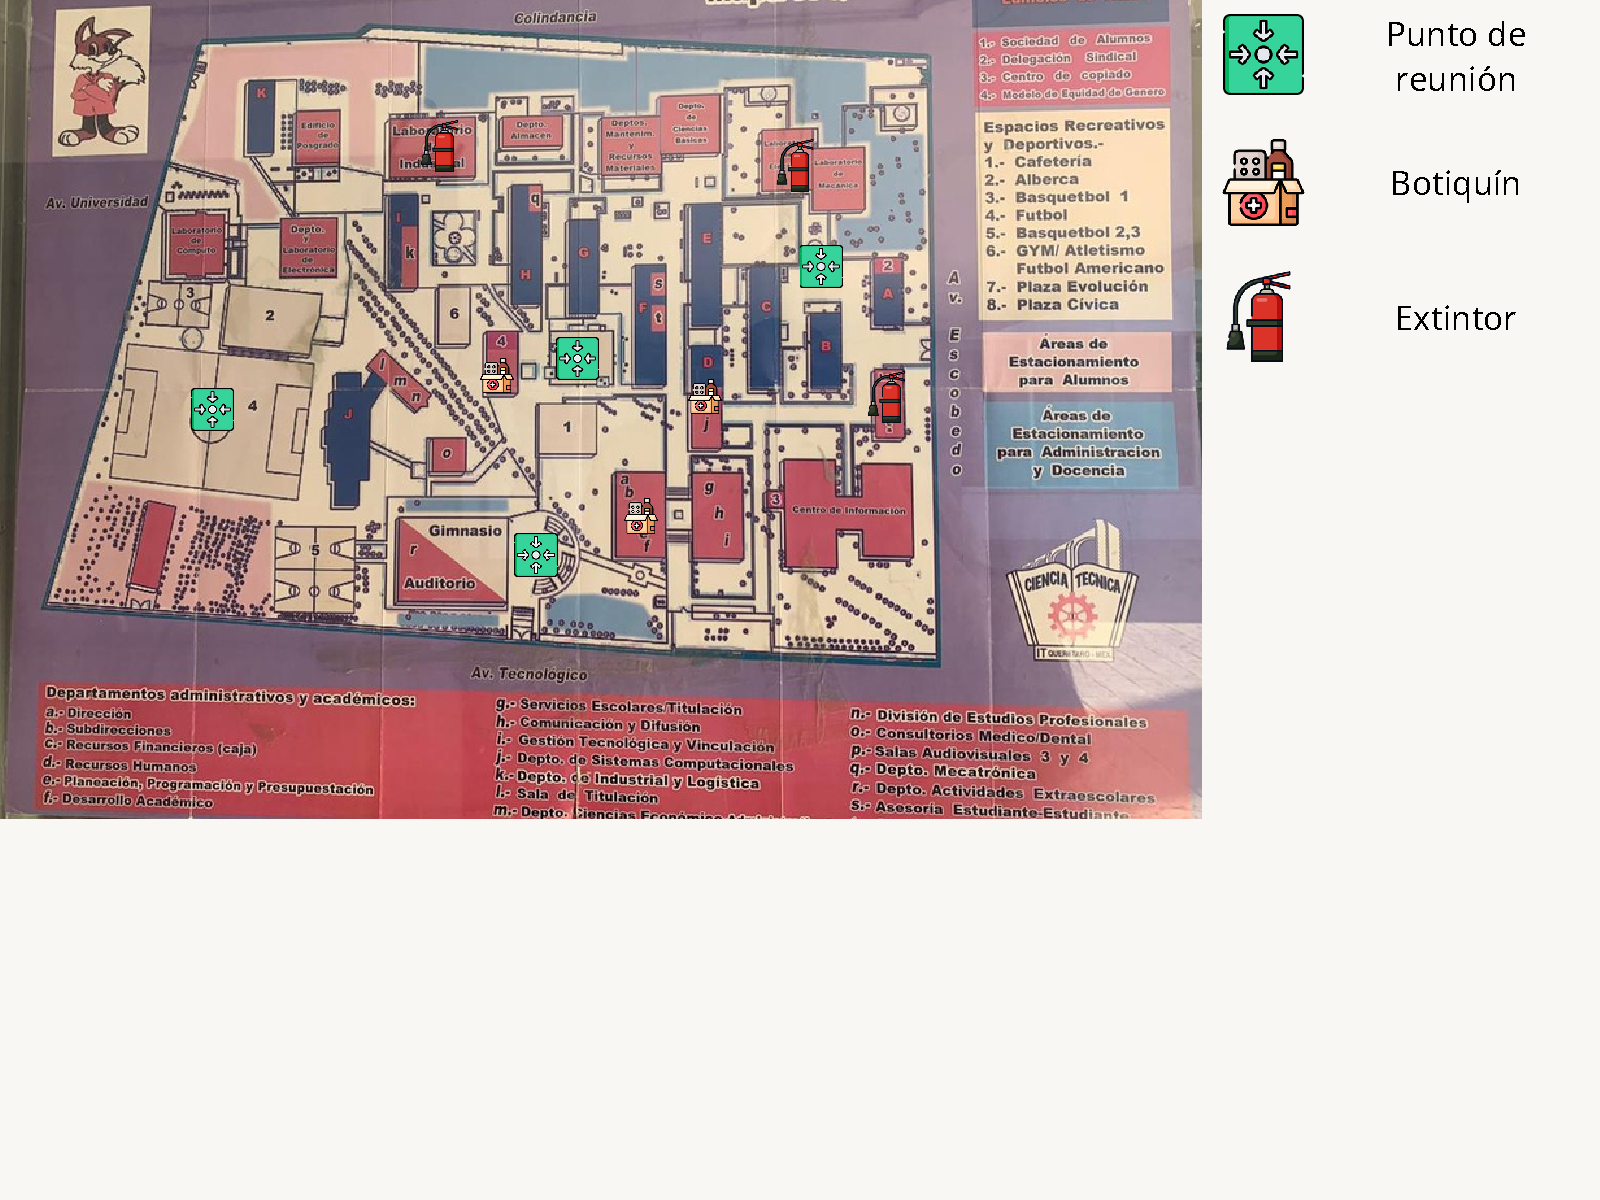
\includegraphics[trim = {15mm 55mm 10mm 3mm},clip,scale=0.40]{16/Img/planoDeRecursos.pdf}
        \caption{Plano de Localización de Recursos}
        \label{Plano de Localización de Recursos}
    \end{figure}
%
%
\subsubsection{Identificación de puntos de reunión}
Los puntos de reunión los podrás ubicar en la figura 19: Plano de Localización de Recursos. \ref{Plano de Localización de Recursos}
\subsubsection{Brigada de evacuación}
%
%
\begin{figure}[H]
        \centering
        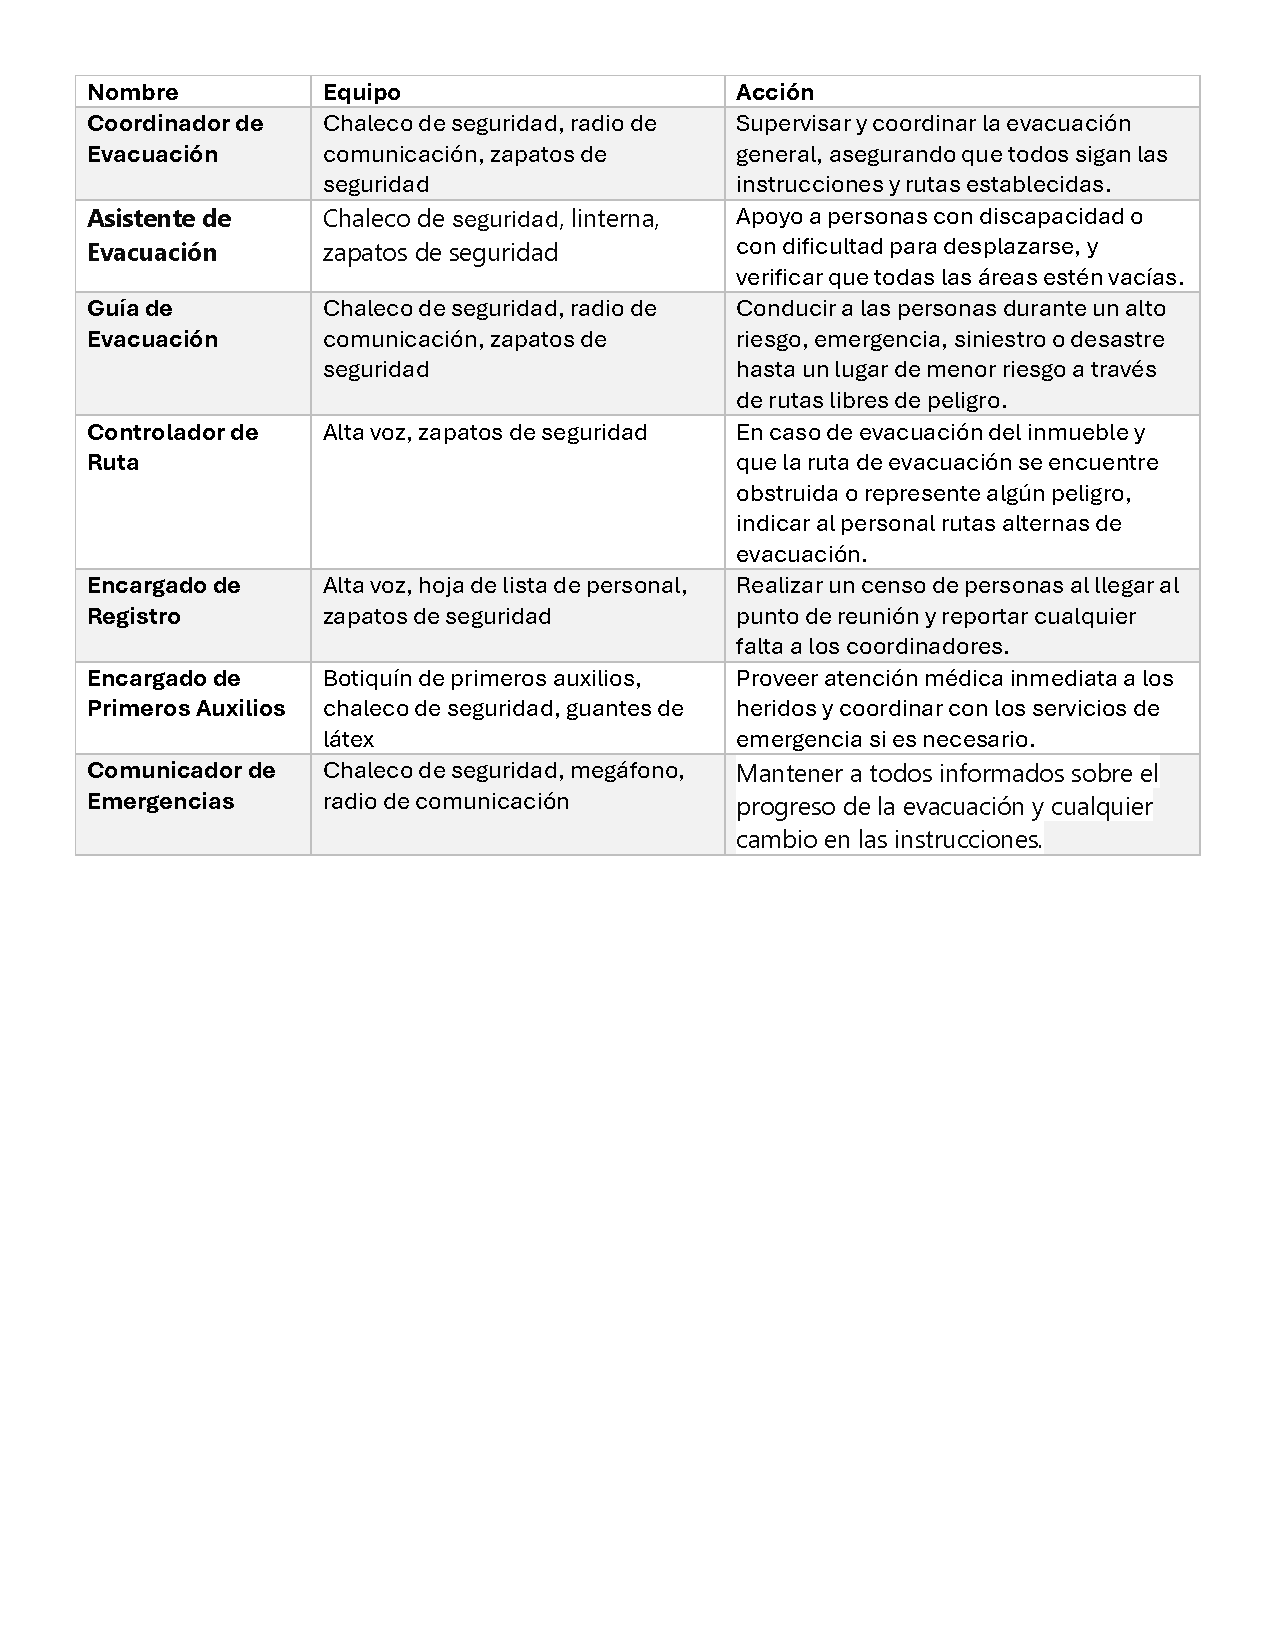
\includegraphics[trim = {15mm 120mm 10mm 3mm},clip,scale=0.43]{16/Img/brigadaDeEvacuacion.pdf}
        \caption{Brigada de Evacuación}
        \label{Brigada de Evacuación}
    \end{figure}
%
%
\subsubsection{Directorio de telefónicos de emergencia}
Un Directorio Telefónico de Emergencia es una lista organizada con números de teléfono de contactos importantes que pueden ser necesarios en situaciones de emergencia. Esta lista es muy útil para asegurar una respuesta rápida y efectiva en caso de incidentes, accidentes, desastres naturales u otras situaciones urgentes.
%
%
\begin{figure}[H]
        \centering
        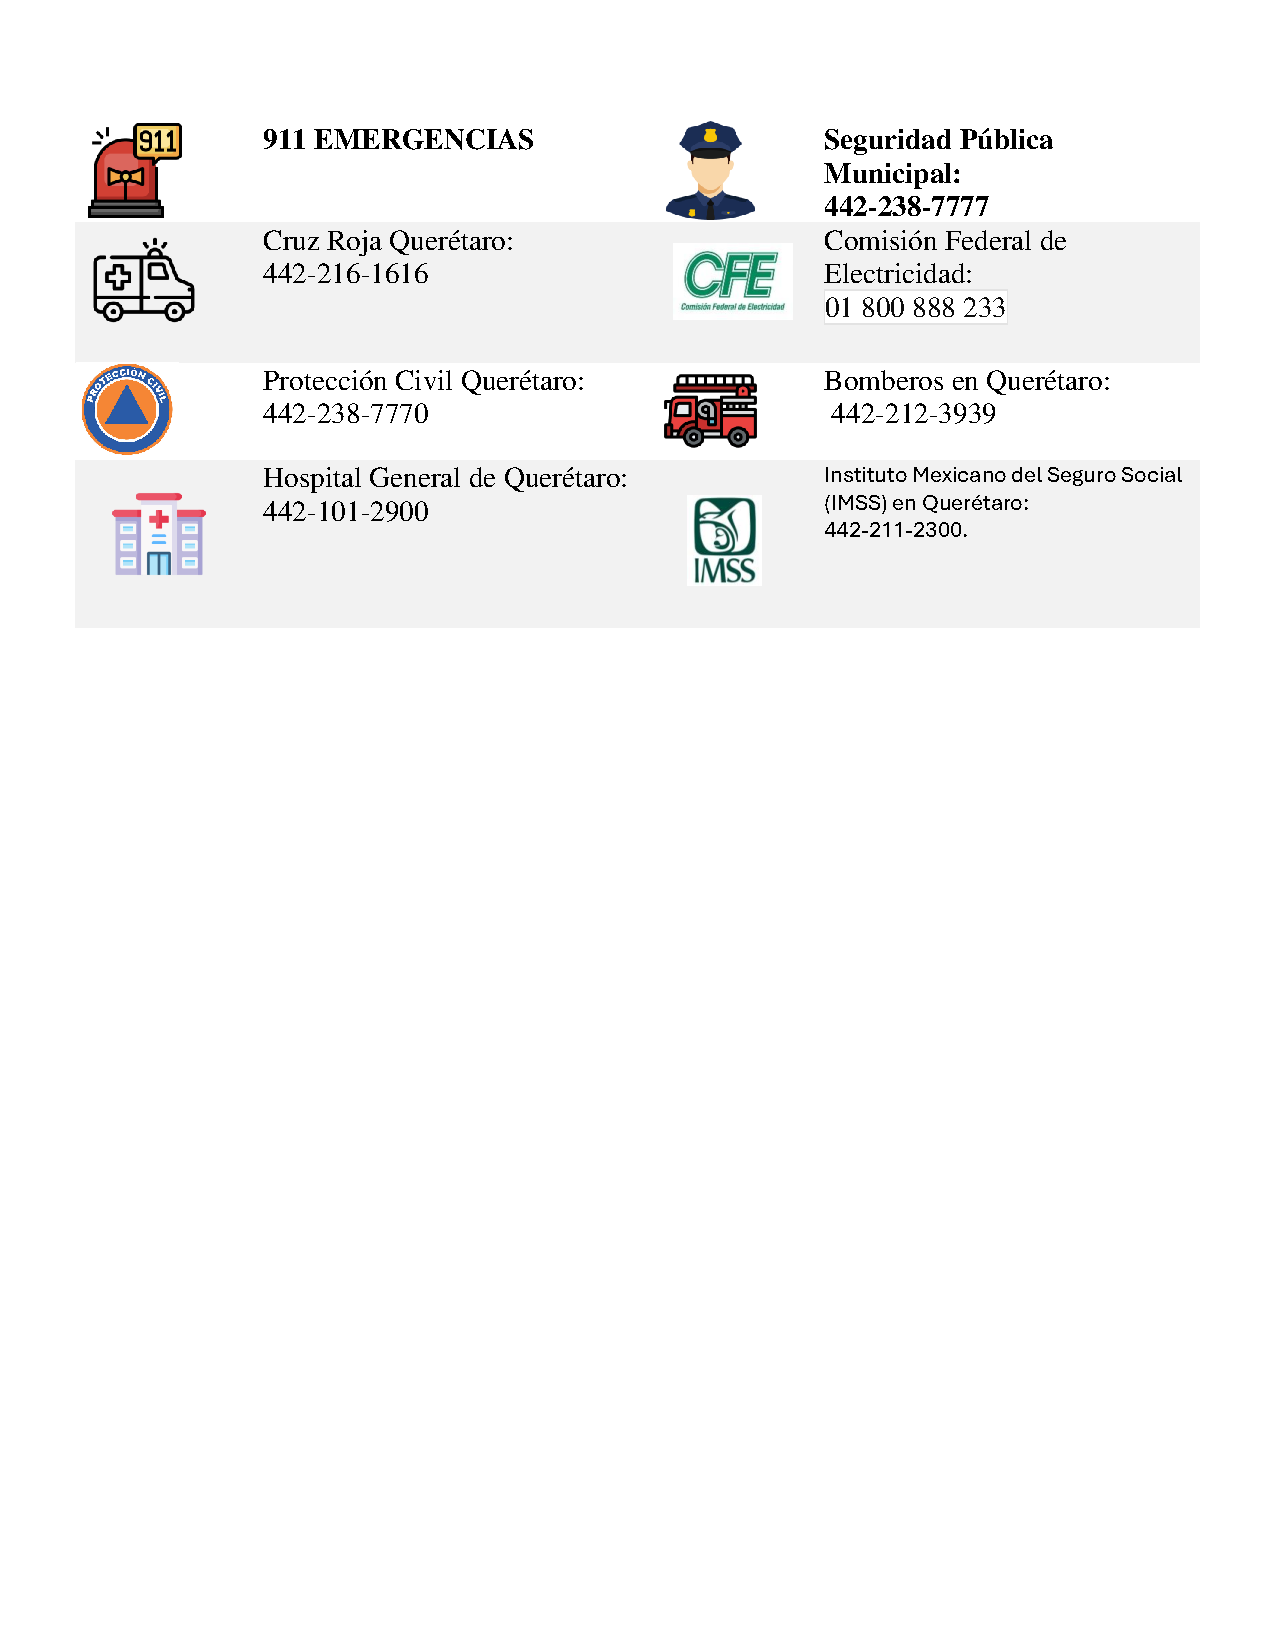
\includegraphics[trim = {15mm 160mm 10mm 3mm},clip,scale=0.43]{16/Img/numerosdeEmergencia.pdf}
        \caption{Directorio de telefónicos de emergencia}
        \label{Directorio de telefónicos de emergencia}
    \end{figure}
%
%
\subsection{Procedimiento Circuito Electrónico}
    % 
    % 
    \begin{figure}[H]
        \centering
        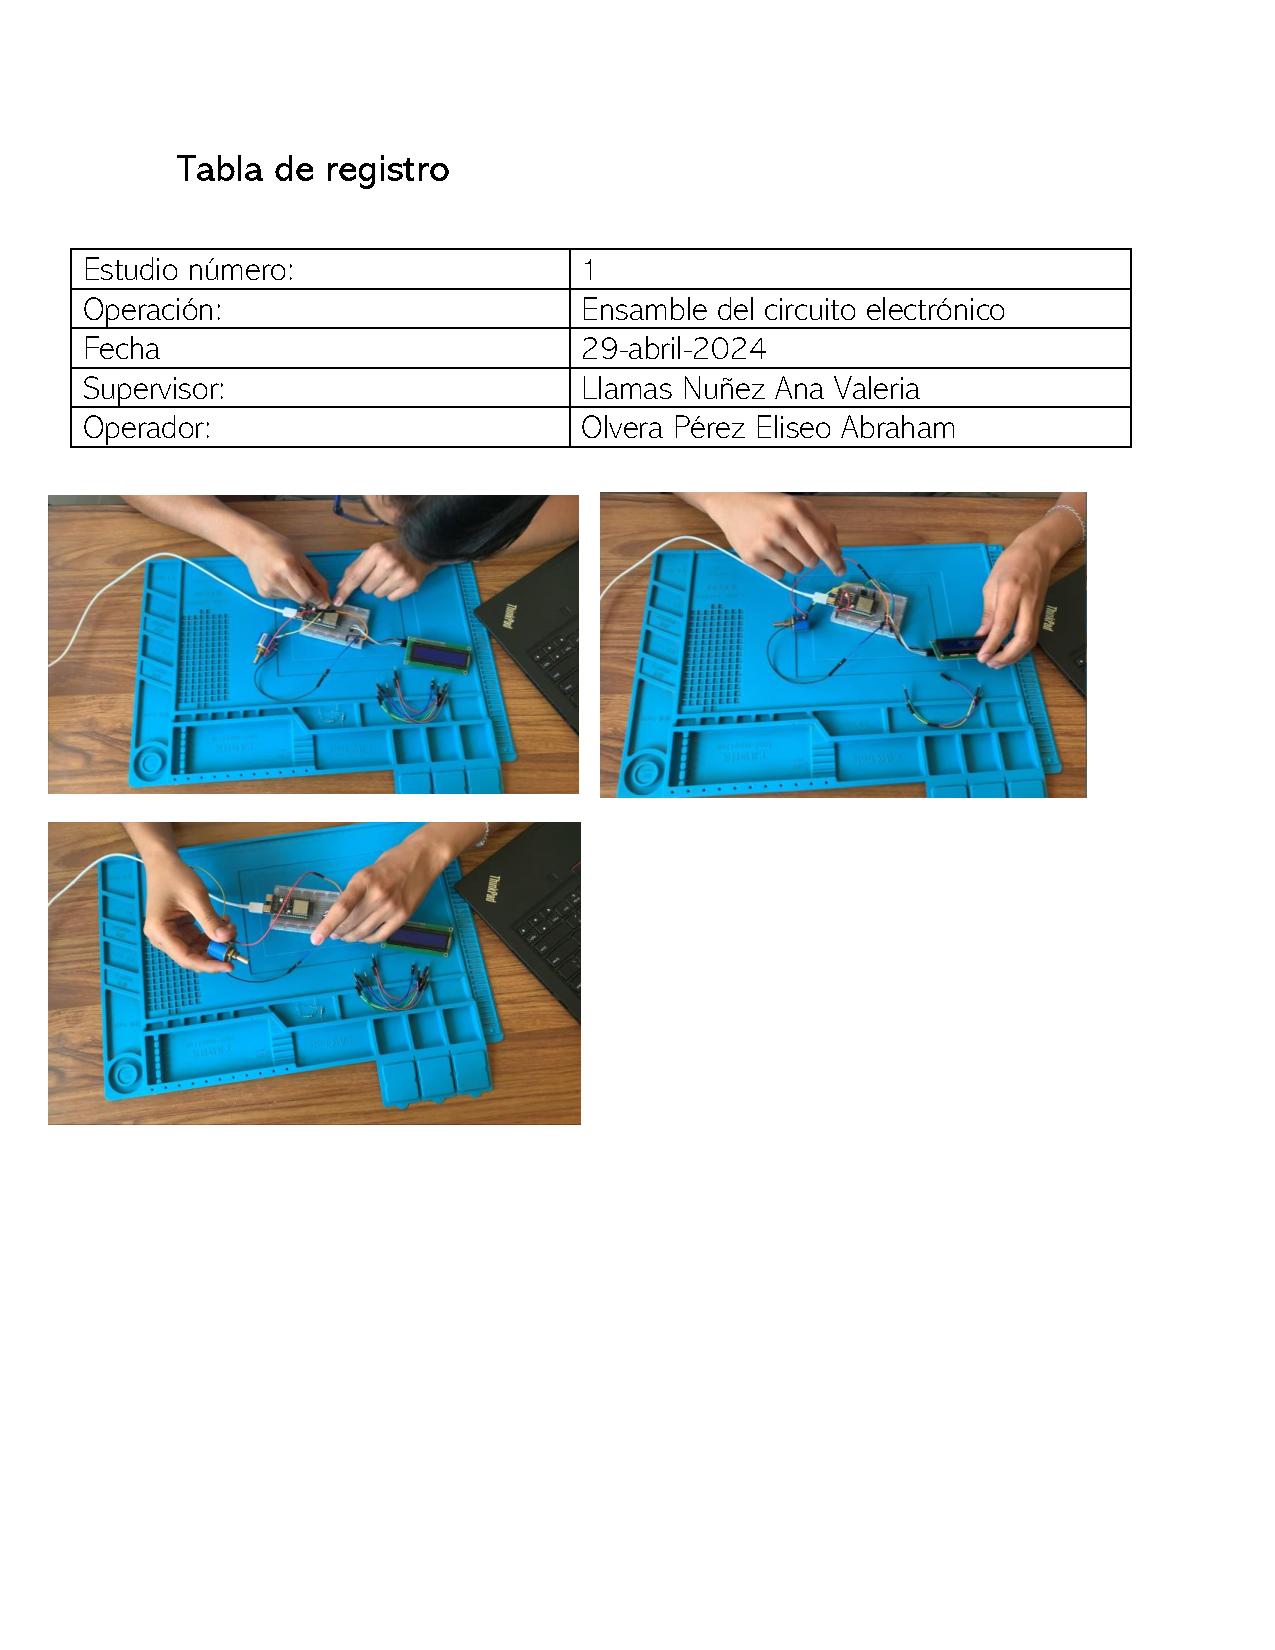
\includegraphics[trim = {12mm 60mm 12mm 40mm},clip,scale=0.5]{16/Img/tablaDeRegistro.pdf}
        \caption{Evidencias}
        \label{fig:Evidencias}
    \end{figure}
    % 
    % 
\subsection{Análisis de los métodos, materiales, herramientas e instalación utilizada en la ejecución del ensamble de un circuito electrónico}
%
%
\begin{figure}[H]
        \centering
        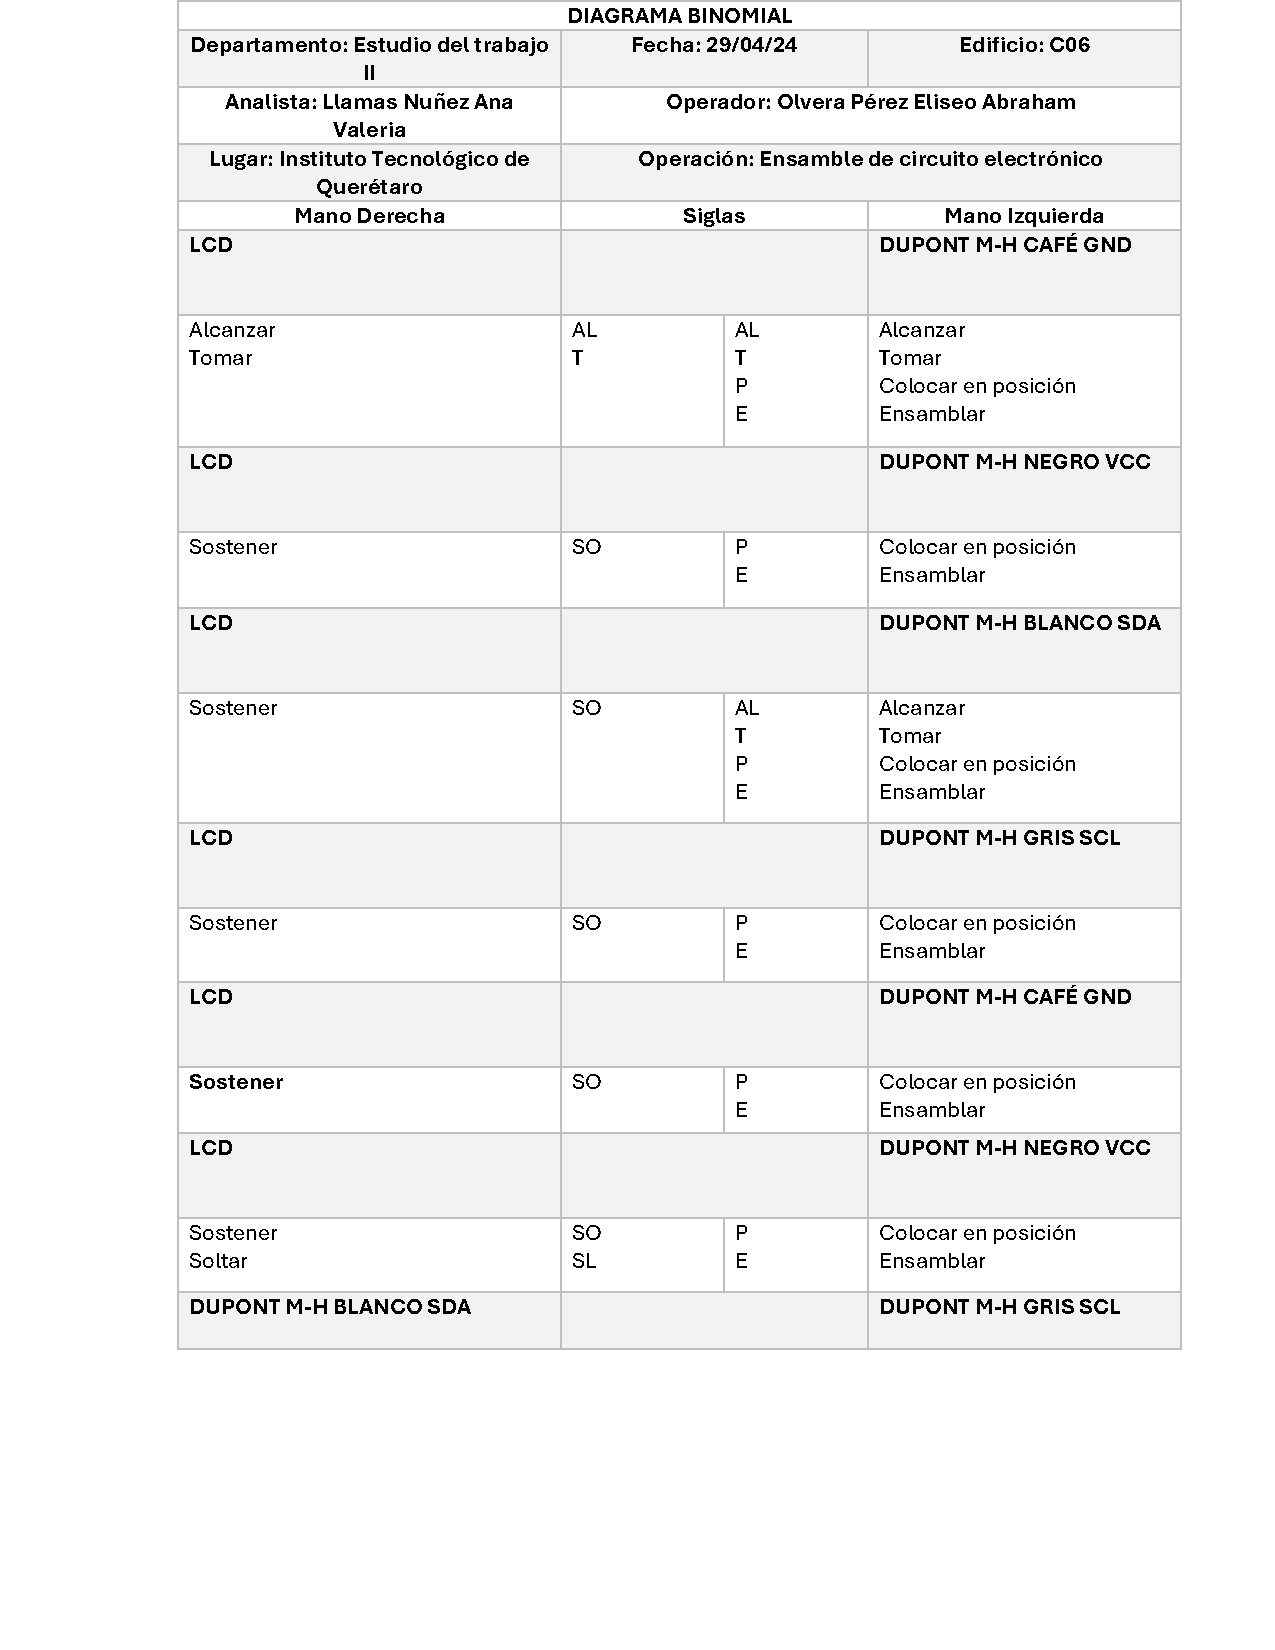
\includegraphics[trim = {5mm 80mm 5mm 10mm},clip,scale=0.40]{16/Img/tablaBimanual.pdf}
        \caption{Tabla Bimanual}
        \label{Tabla Bimanual}
    \end{figure}
%
%
\subsubsection{Datos estándar continuos y discretos}
En nuestra operación determinamos diferentes actividades obteniendo tiempos distintos para cada actividad. 
Dentro de esta tomamos nuestra desviación estándar para determinar nuestras holguras ya que nos ayuda ver la dispersión o variabilidad de un conjunto de datos.
En el muestreo que tomamos con todos los compañeros para determinar las holguras de igual manera ocupe la desviación estándar, a diferencia del anterior  donde saque el promedio de ambas muestras (2 vídeos) en el muestreo general, tome mi límite inferior (el valor más pequeño del tiempo ciclo individual) y el límite superior (el valor más grande del tiempo ciclo individual) para así poder determinar mi desviación estándar, para el tiempo estándar sume el tiempo de ciclo total inicial más la desviación estándar.
% 
% 
    \begin{figure}[H]
        \centering
        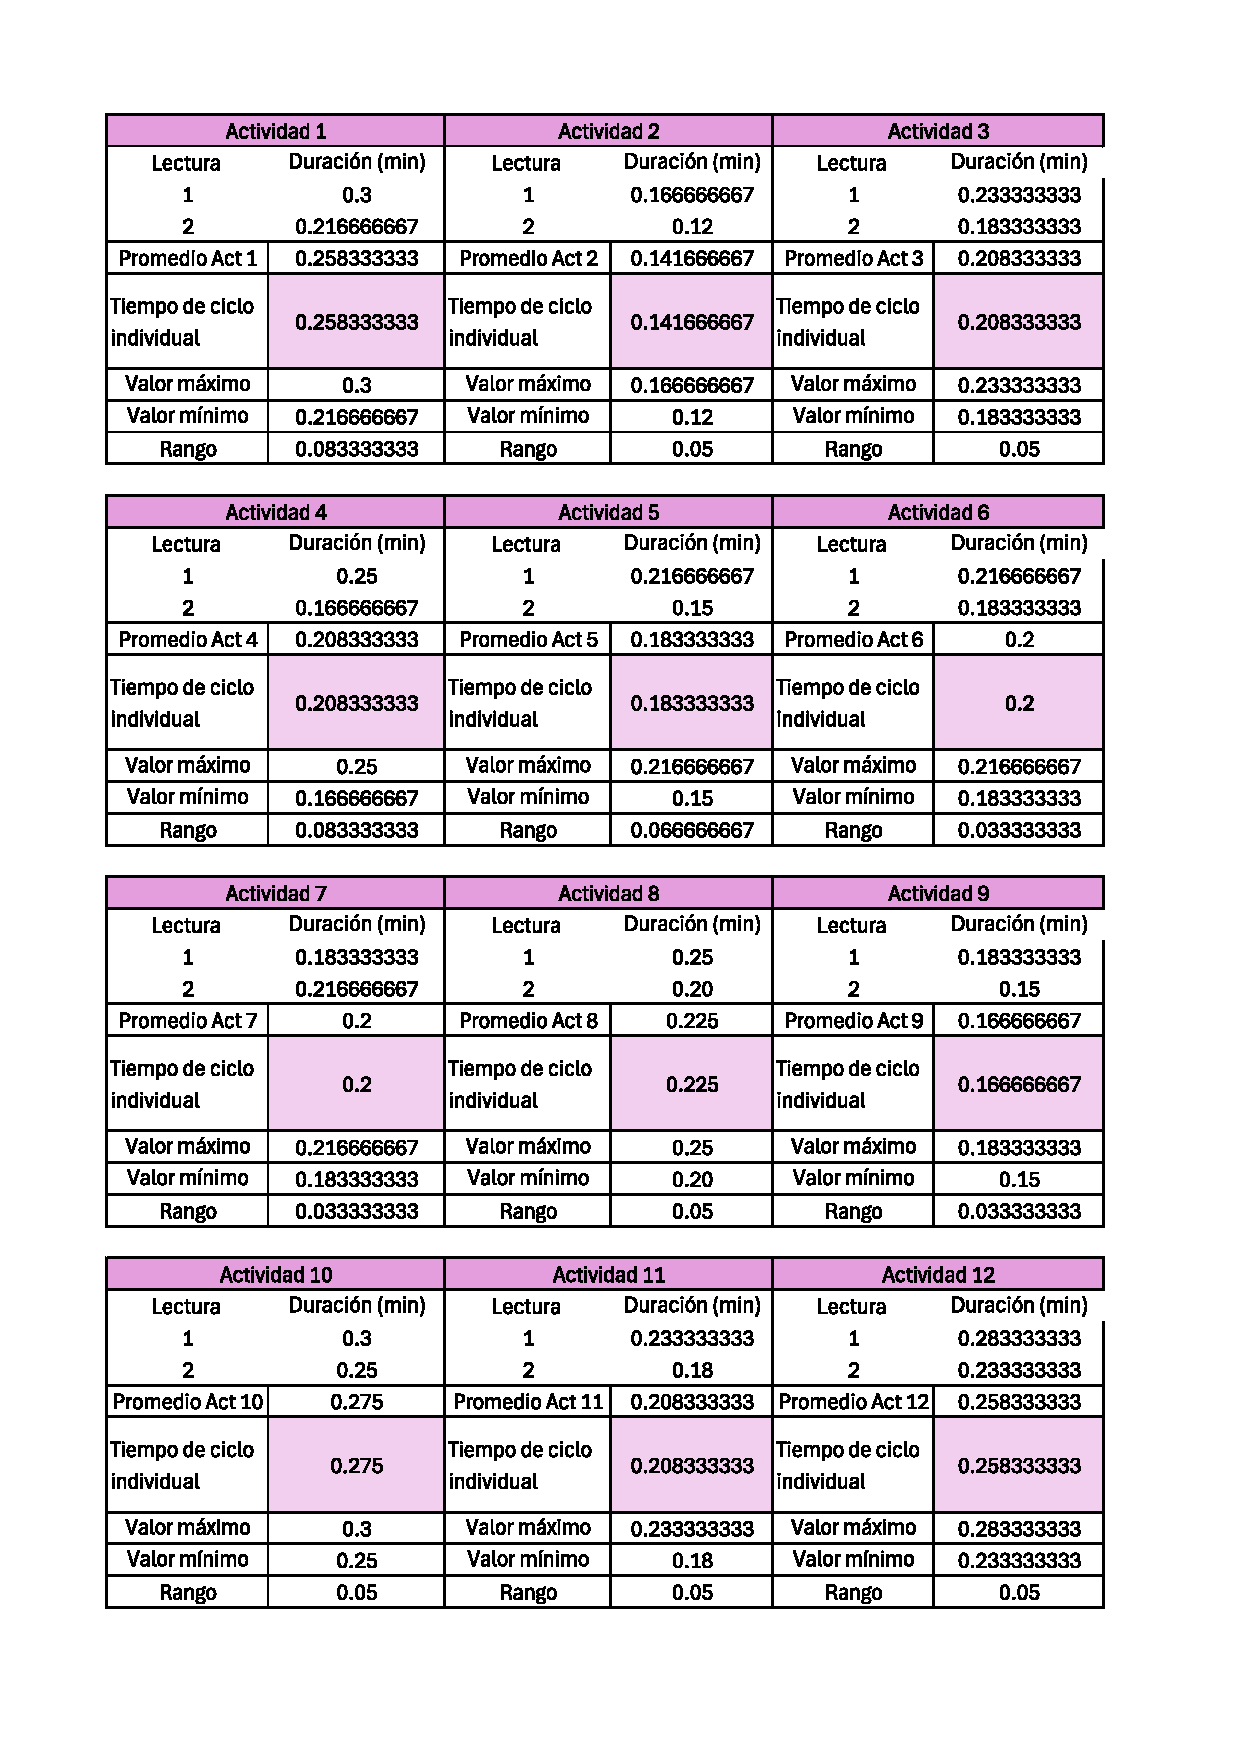
\includegraphics[trim = {5mm 15mm 5mm 
        0mm},clip,scale=0.45]{16/Img/datosEstandar.pdf}
        \caption{Datos y tiempo ciclo}
        \label{fig:Datos y tiempo ciclo}
    \end{figure}
    % 
    % 
    \begin{figure}[H]
        \centering
        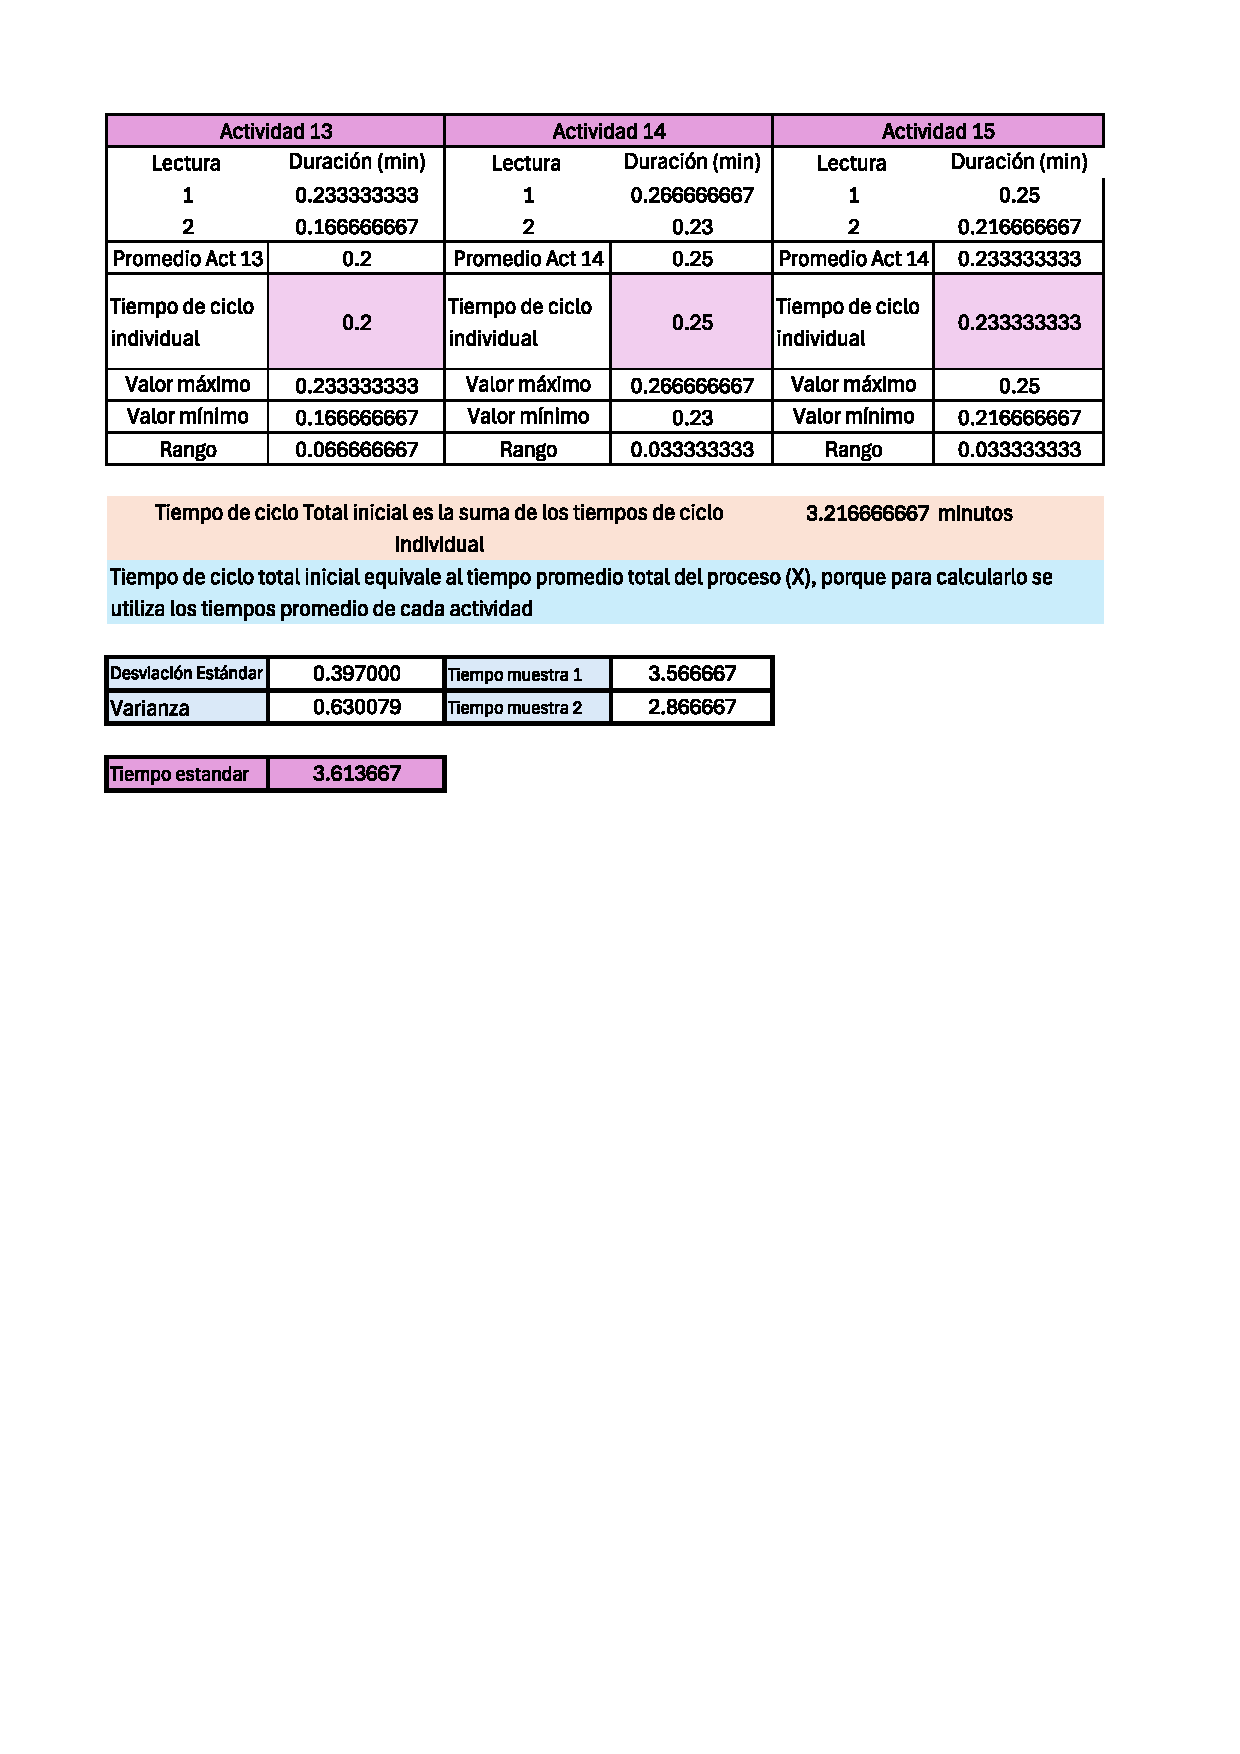
\includegraphics[trim = {15mm 160mm 20mm 
        40mm},clip,scale=0.35]{16/Img/tiempoEstandarM.pdf}
        \caption{Tiempo estándar}
        \label{fig:Tiempo estándar}
    \end{figure}
   
     \begin{figure}[H]
        \centering
        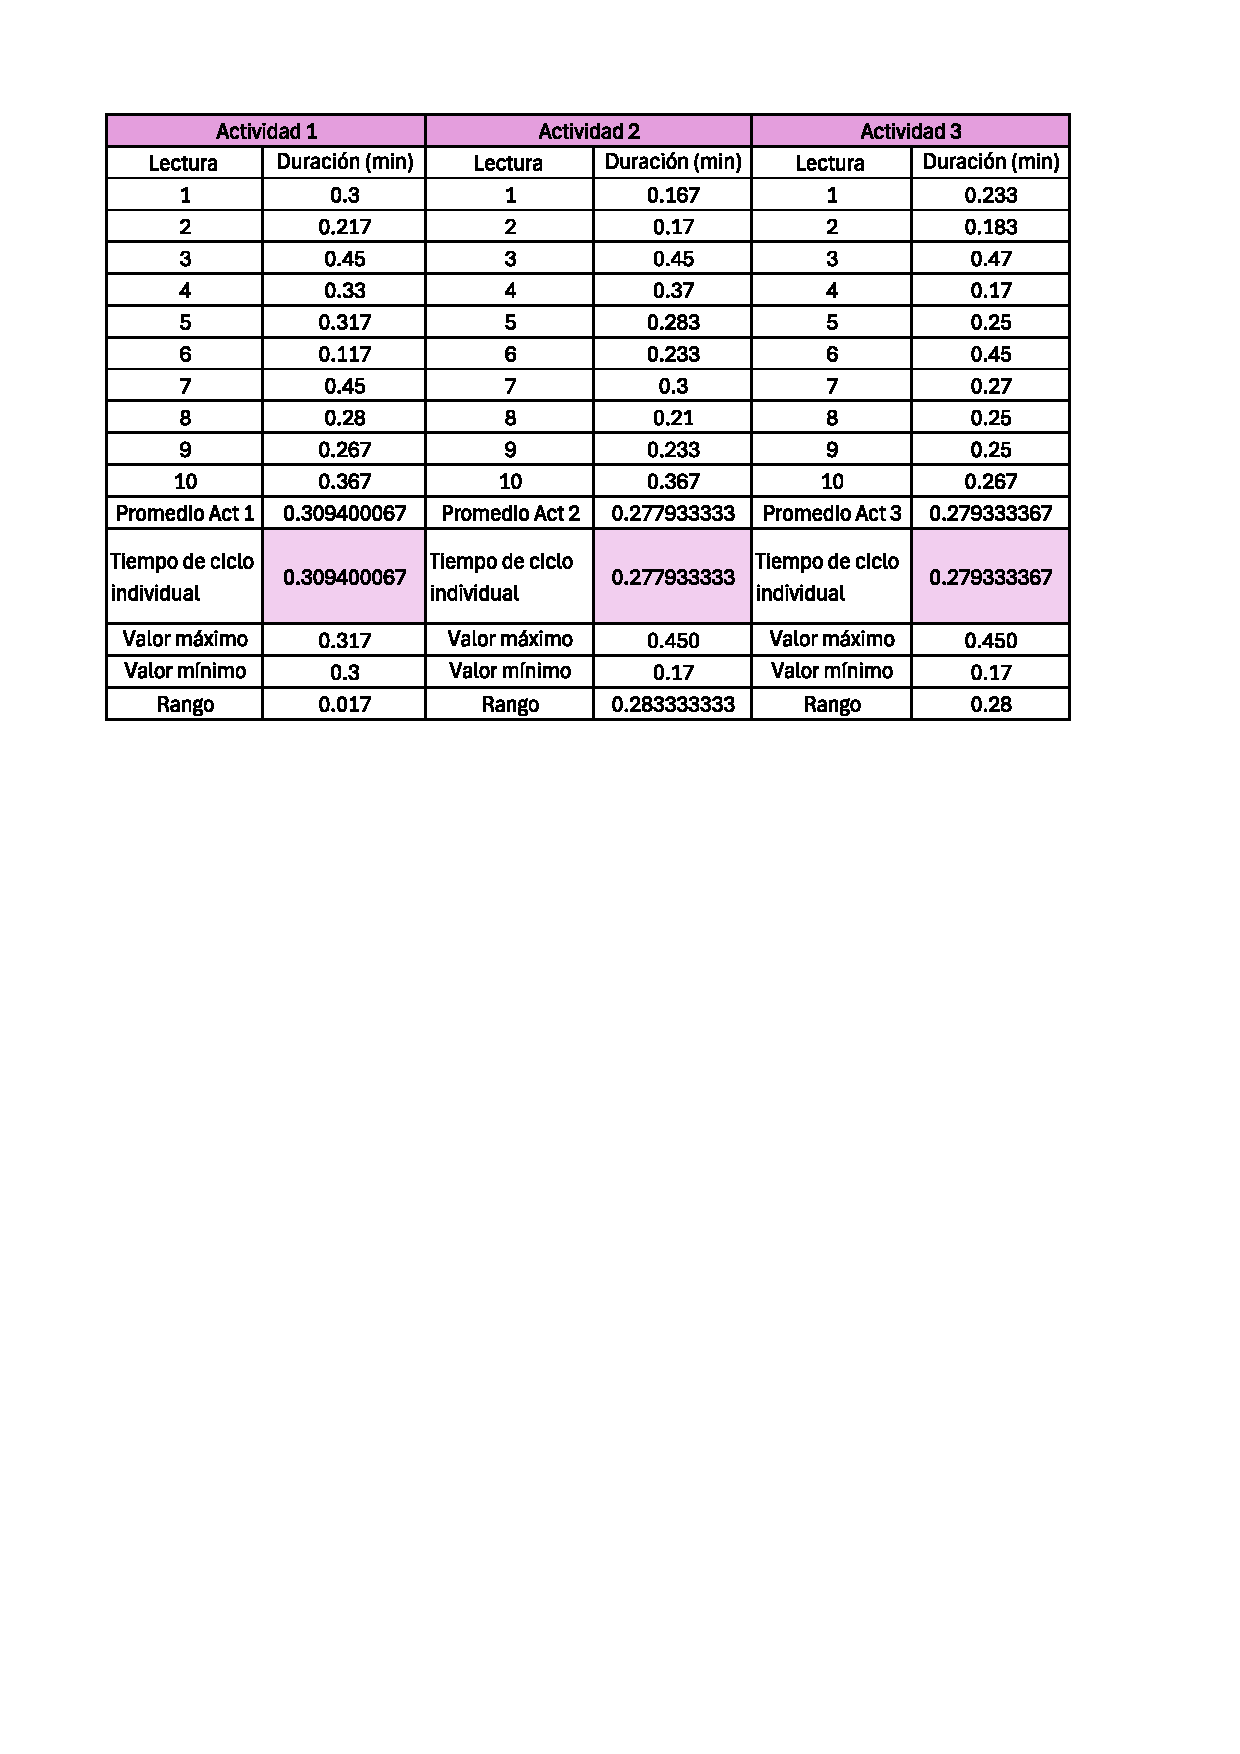
\includegraphics[trim = {15mm 160mm 20mm 
        5mm},clip,scale=0.4]{16/Img/muestreo1}
        \caption{Datos y tiempo ciclo 1}
        \label{fig:Datos y tiempo ciclo 1}
    \end{figure}
    
    \begin{figure}[H]
        \centering
        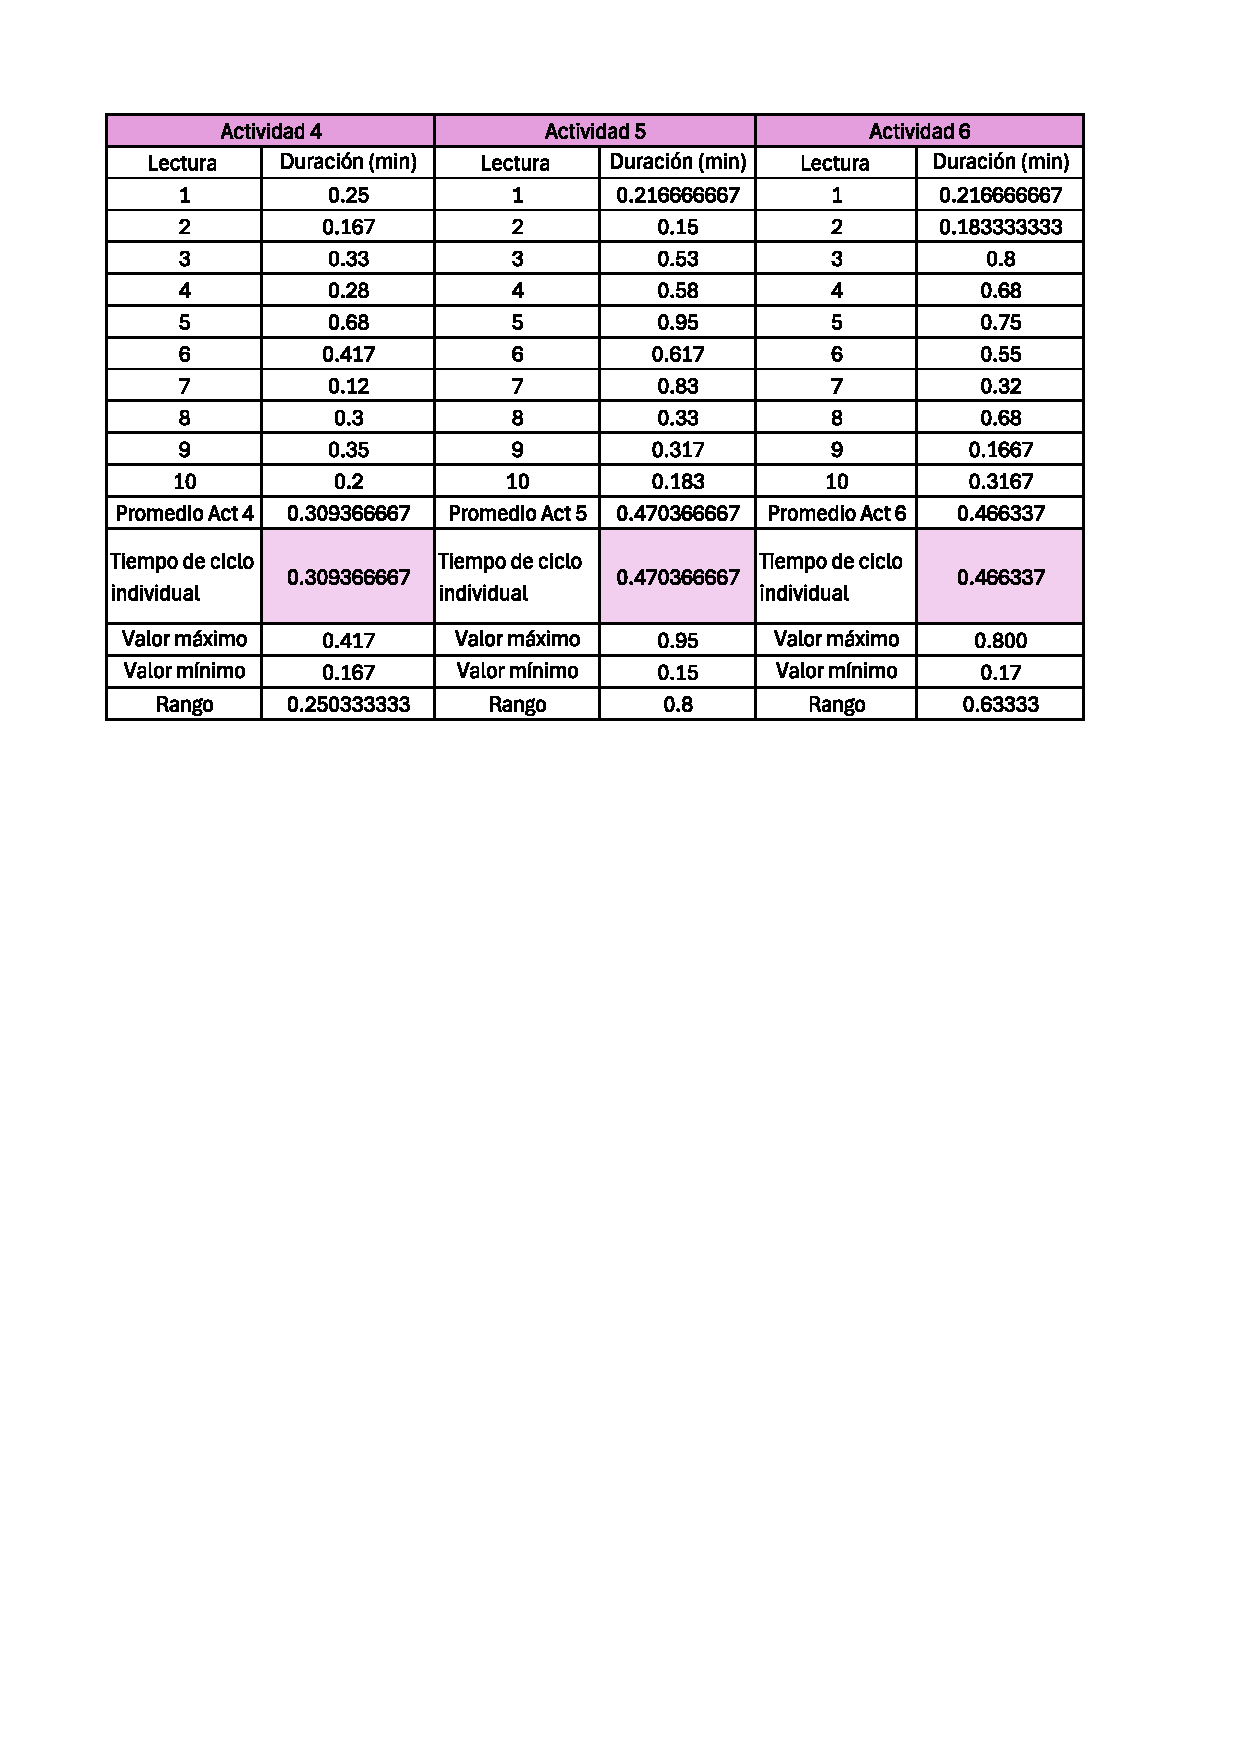
\includegraphics[trim = {15mm 160mm 20mm 
        0mm},clip,scale=0.4]{16/Img/muestreo2}
        \caption{Datos y tiempo ciclo 2}
        \label{fig:Datos y tiempo ciclo 2}
         \end{figure}
         
    \begin{figure}[H]
        \centering
        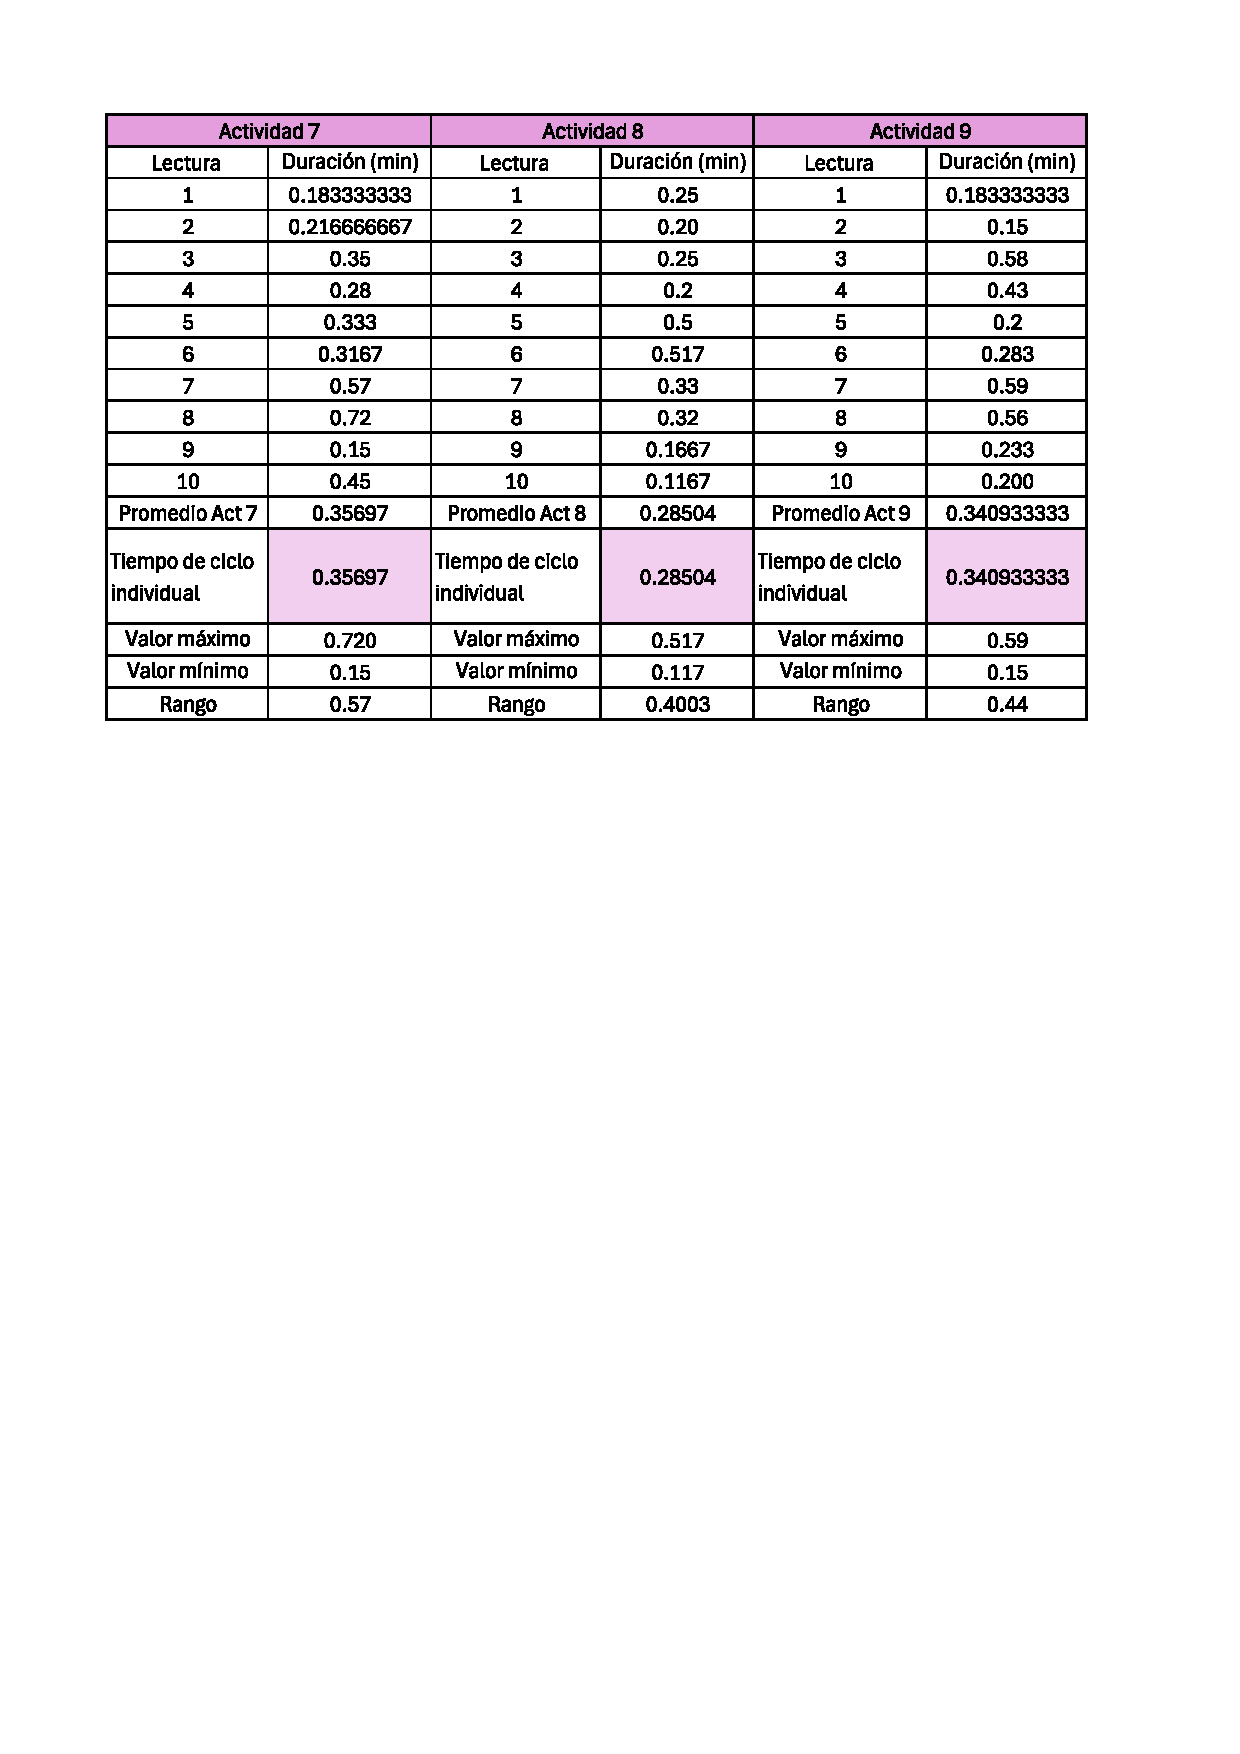
\includegraphics[trim = {15mm 160mm 20mm 
        0mm},clip,scale=0.4]{16/Img/muestreo3}
        \caption{Datos y tiempo ciclo 3}
        \label{fig:Datos y tiempo ciclo 3}
         \end{figure}
    
    \begin{figure}[H]
        \centering
        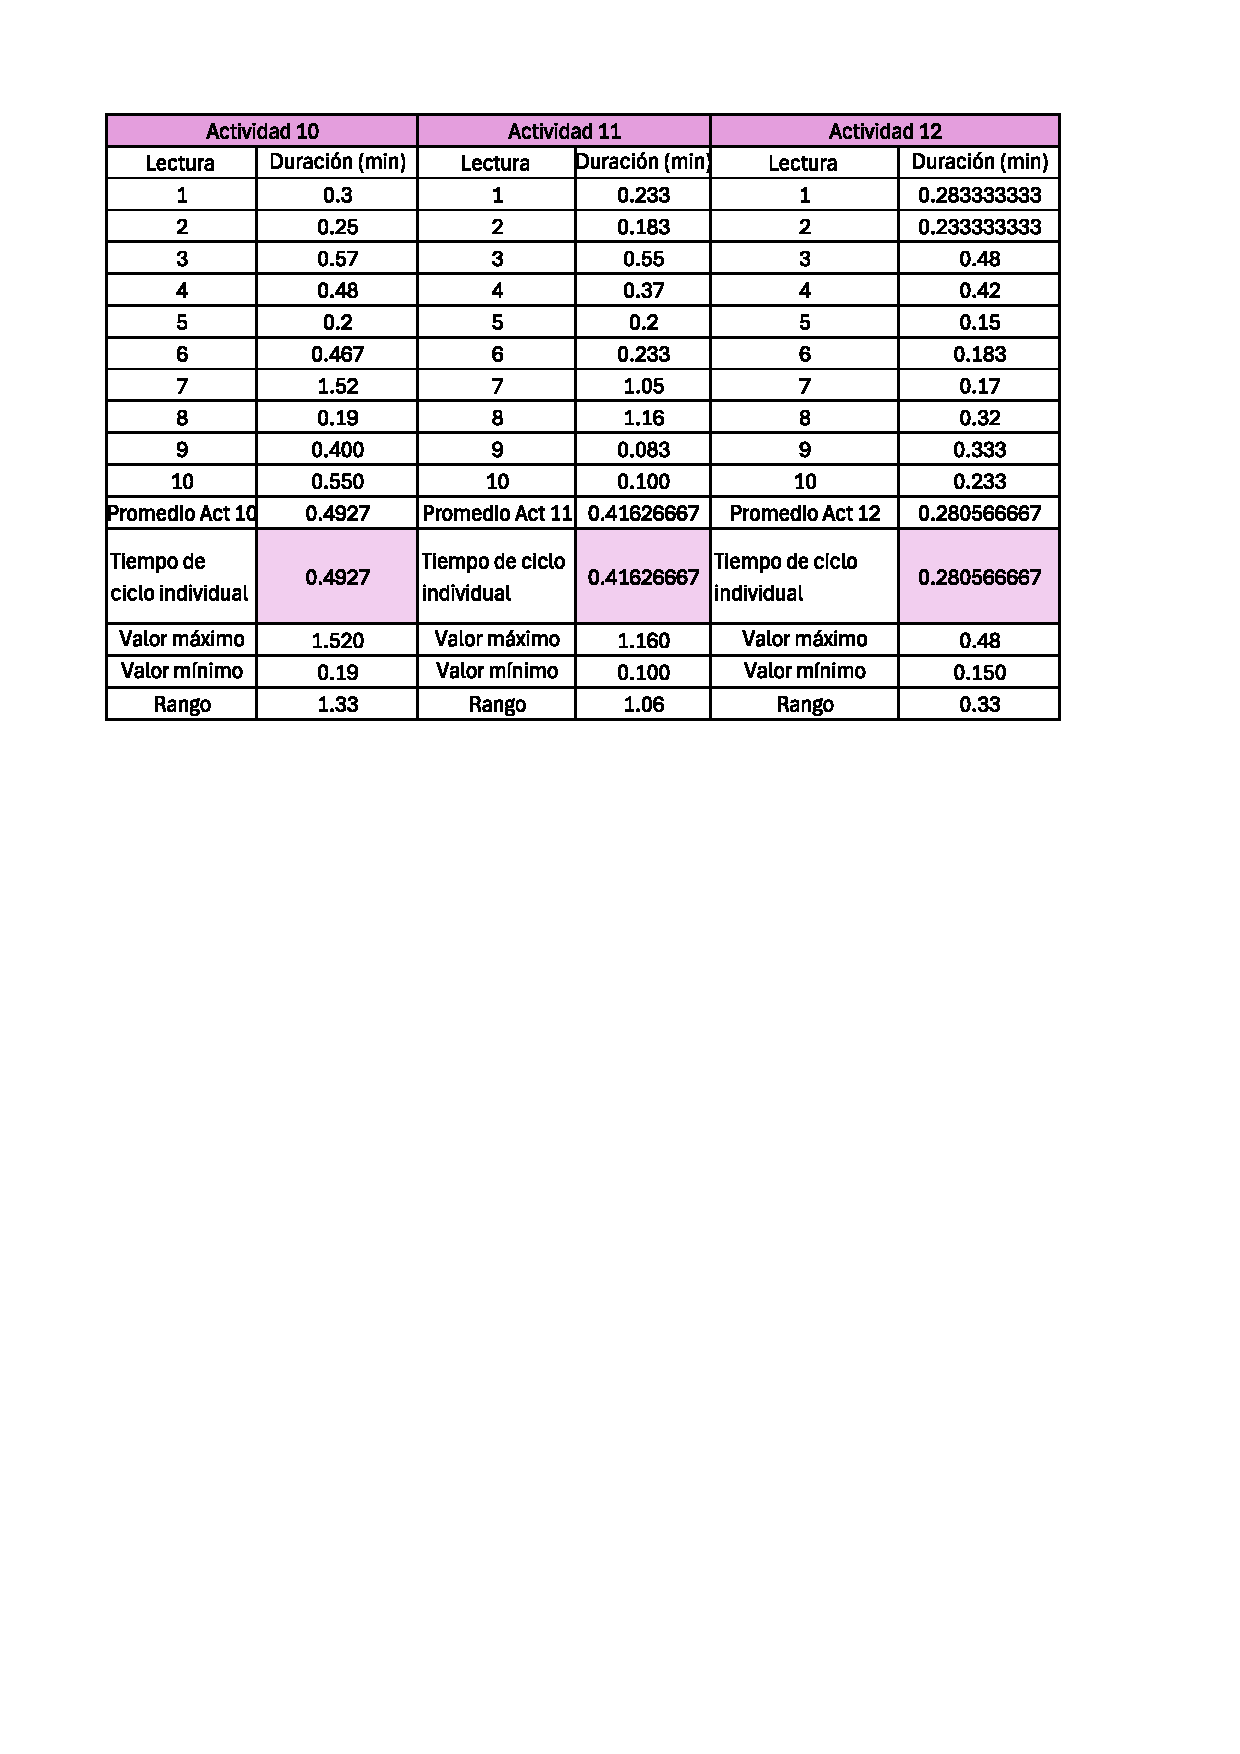
\includegraphics[trim = {15mm 160mm 20mm 
        0mm},clip,scale=0.4]{16/Img/muestreo4}
        \caption{Datos y tiempo ciclo 4}
        \label{fig:Datos y tiempo ciclo 4}
         \end{figure}
    
    \begin{figure}[H]
        \centering
        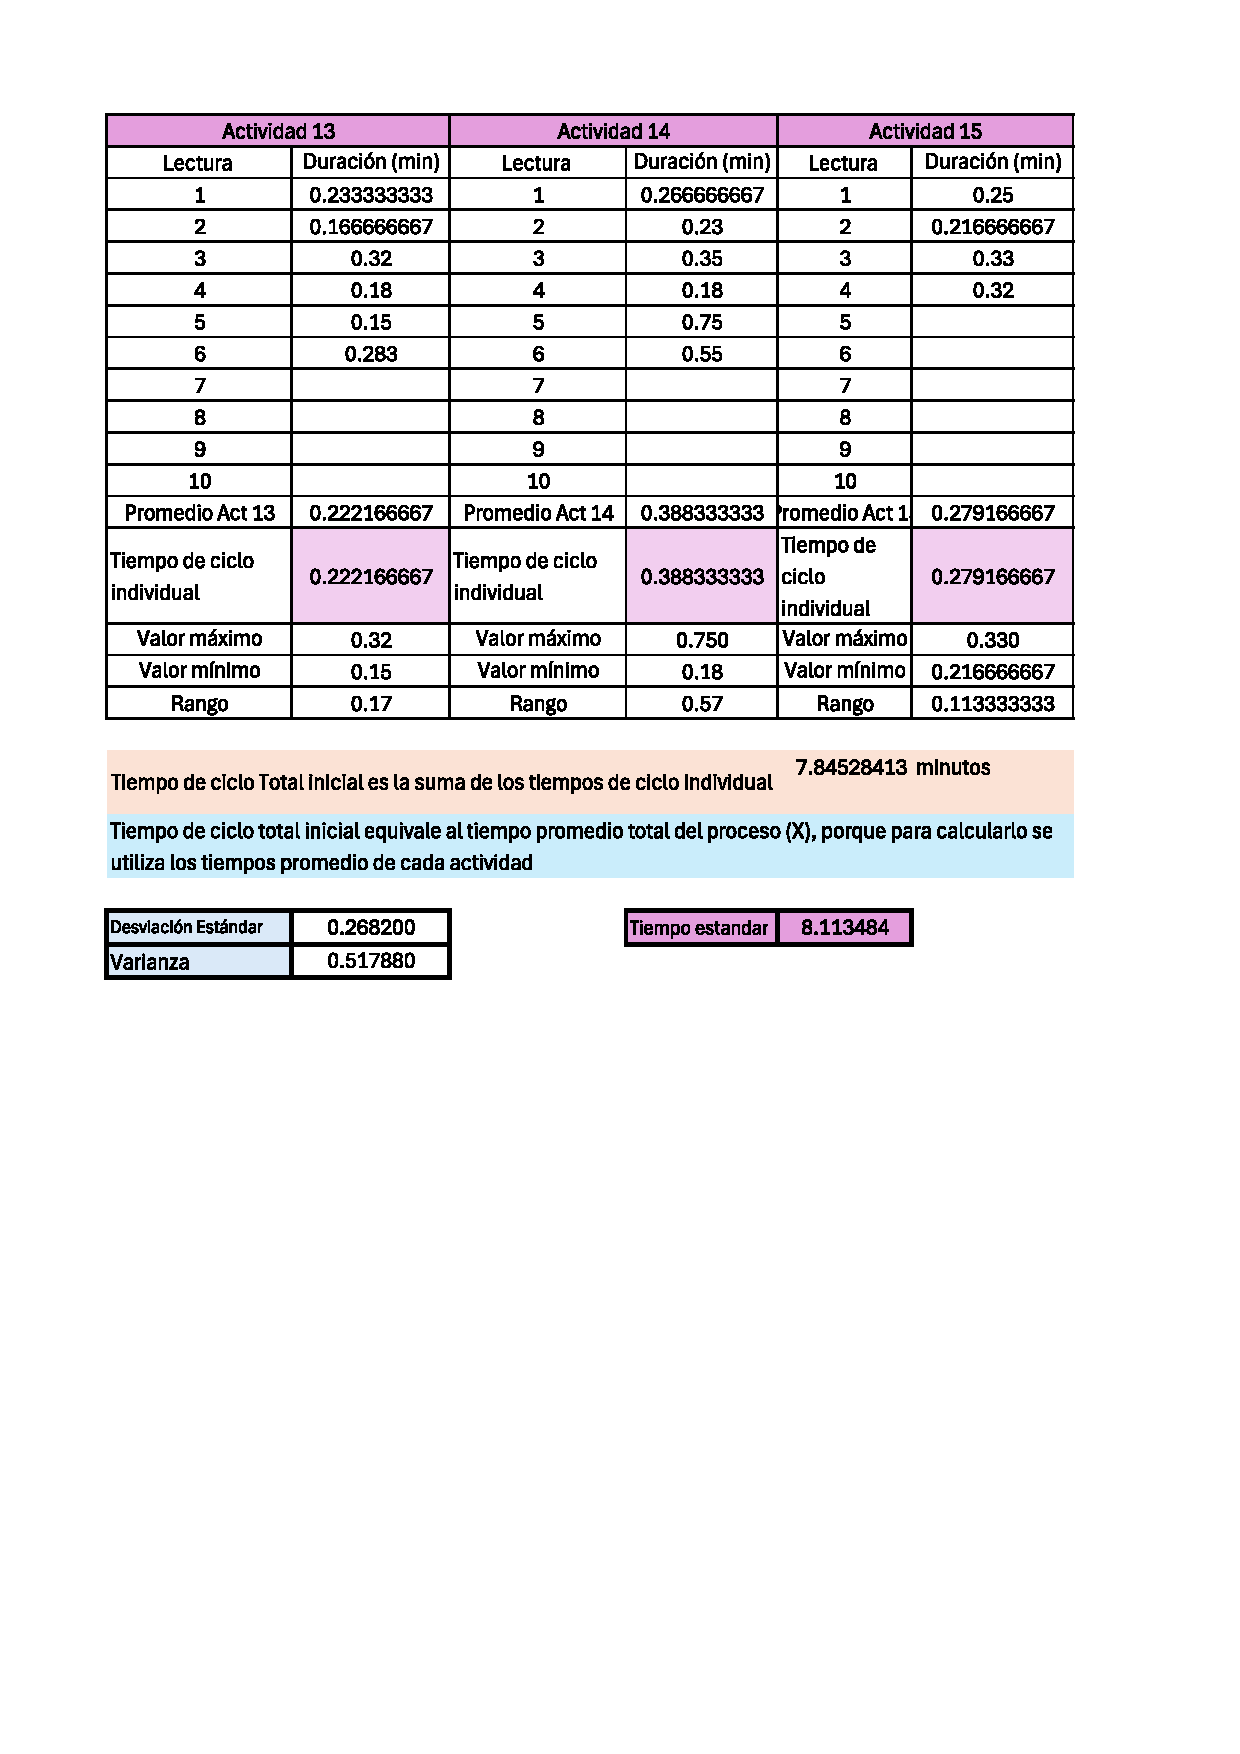
\includegraphics[trim = {15mm 100mm 20mm 
        0mm},clip,scale=0.4]{16/Img/muestreo5}
        \caption{Datos y tiempo ciclo 5}
        \label{fig:Datos y tiempo ciclo 5}
         \end{figure}
         
    \begin{figure}[H]
        \centering
        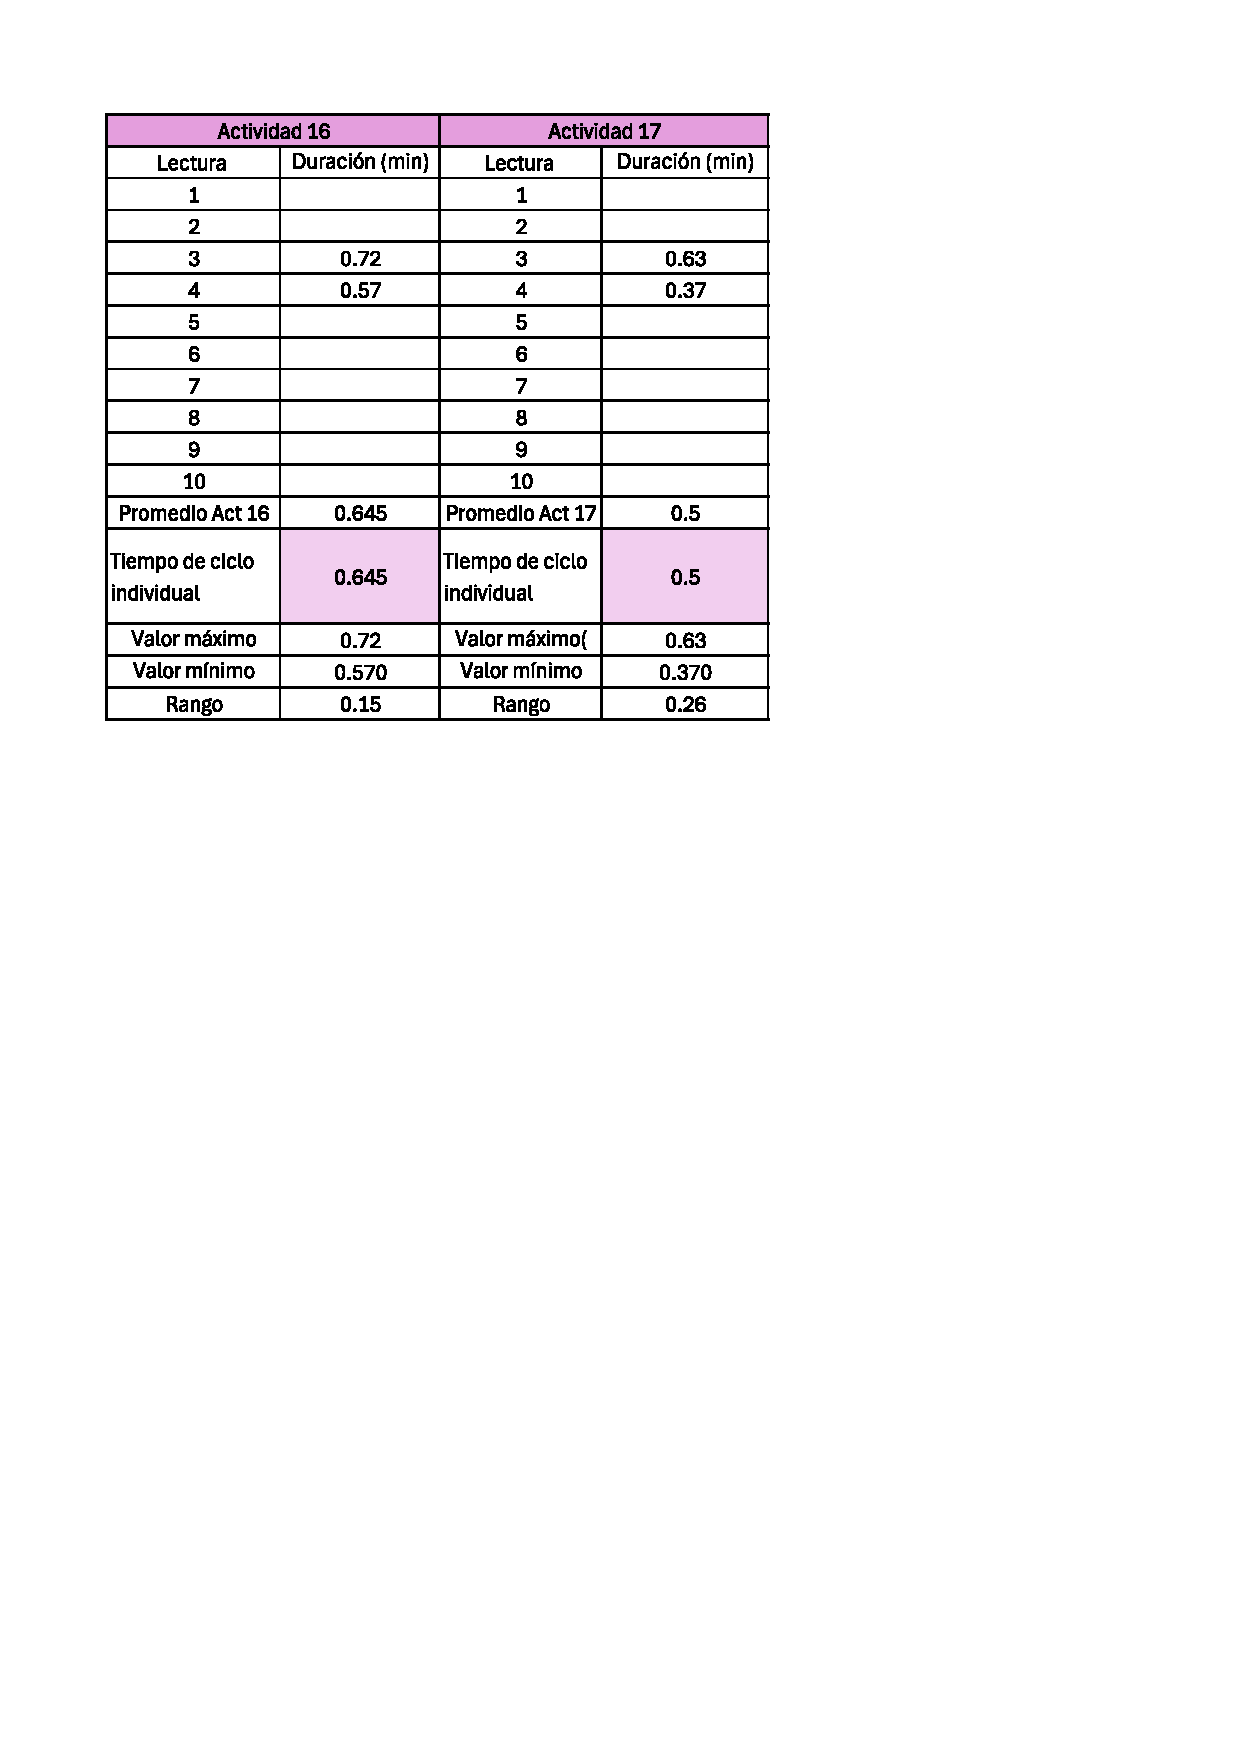
\includegraphics[trim = {15mm 100mm 20mm 
        0mm},clip,scale=0.4]{16/Img/muestreo6}
        \caption{Datos y tiempo ciclo 6}
        \label{fig:Datos y tiempo ciclo 6}
         \end{figure}
    \section{Conclusiones}
    
  En base al conjunto de principios que permiten ordenar la secuencia de pasos para conectar el circuito electrónico, tenemos que aplicar los 3 pasos en los que están basados los STP. Logrando así, que en base a nuestras 2 muestras, PODEMOS sacar el tiempo promedio, para nosotros poder determinar el tiempo estimado que consideramos para realizar el trabajo. de la misma manera, apoyándonos Y basándonos en la metodología de Los therblings nos ayudarán a eliminar movimientos innecesarios, lo cual nos reducirá el tiempo de operación, siendo así que si reducimos el tiempo se reducirán los costos de operación, dando lugar a la primera etapa del estudio de tiempos y movimientos que nos habla de encontrar la forma más económica de hacer el trabajo, concluyendo y ejecutando las acciones empleadas correctamente,podemos considerar que nuestra hipótesis se cumplió con el resultado deseado.
    
    \section{Agradecimientos}
    
    Es importante darles su debido reconocimiento a los laboratorios, instituciones, organizaciones, entre otros que han sido participes para la culminación de este trabajo. También es importante mencionar, fondos, proyectos, becas, entre otros que se le han otorgado al o los autores para realizar el trabajo de investigación. Ejemplo: “Los autores agradecen al Concejo Nacional de Ciencia y Tecnología por los recursos otorgados…”
    
    \section*{Referencias}
    
    \bibliographystyle{ieeetr}
    \bibliography{16/referencias}
    % 
    % 
    %%%%%%%%%%%%%%%%%%%%%%%%%%%%%%%%%%
    \appendix
    %%%%%%%%%%%%%%%%%%%%%%%%%%%%%%%%%%
    % 
    % 
    %%%%%%%%%%%%%%%%%%%%%%%%%%%%%%%%%%
%\centering{\section[\appendixautorefname{}]{Apéndice}}\label{anexo:materialesCE}
%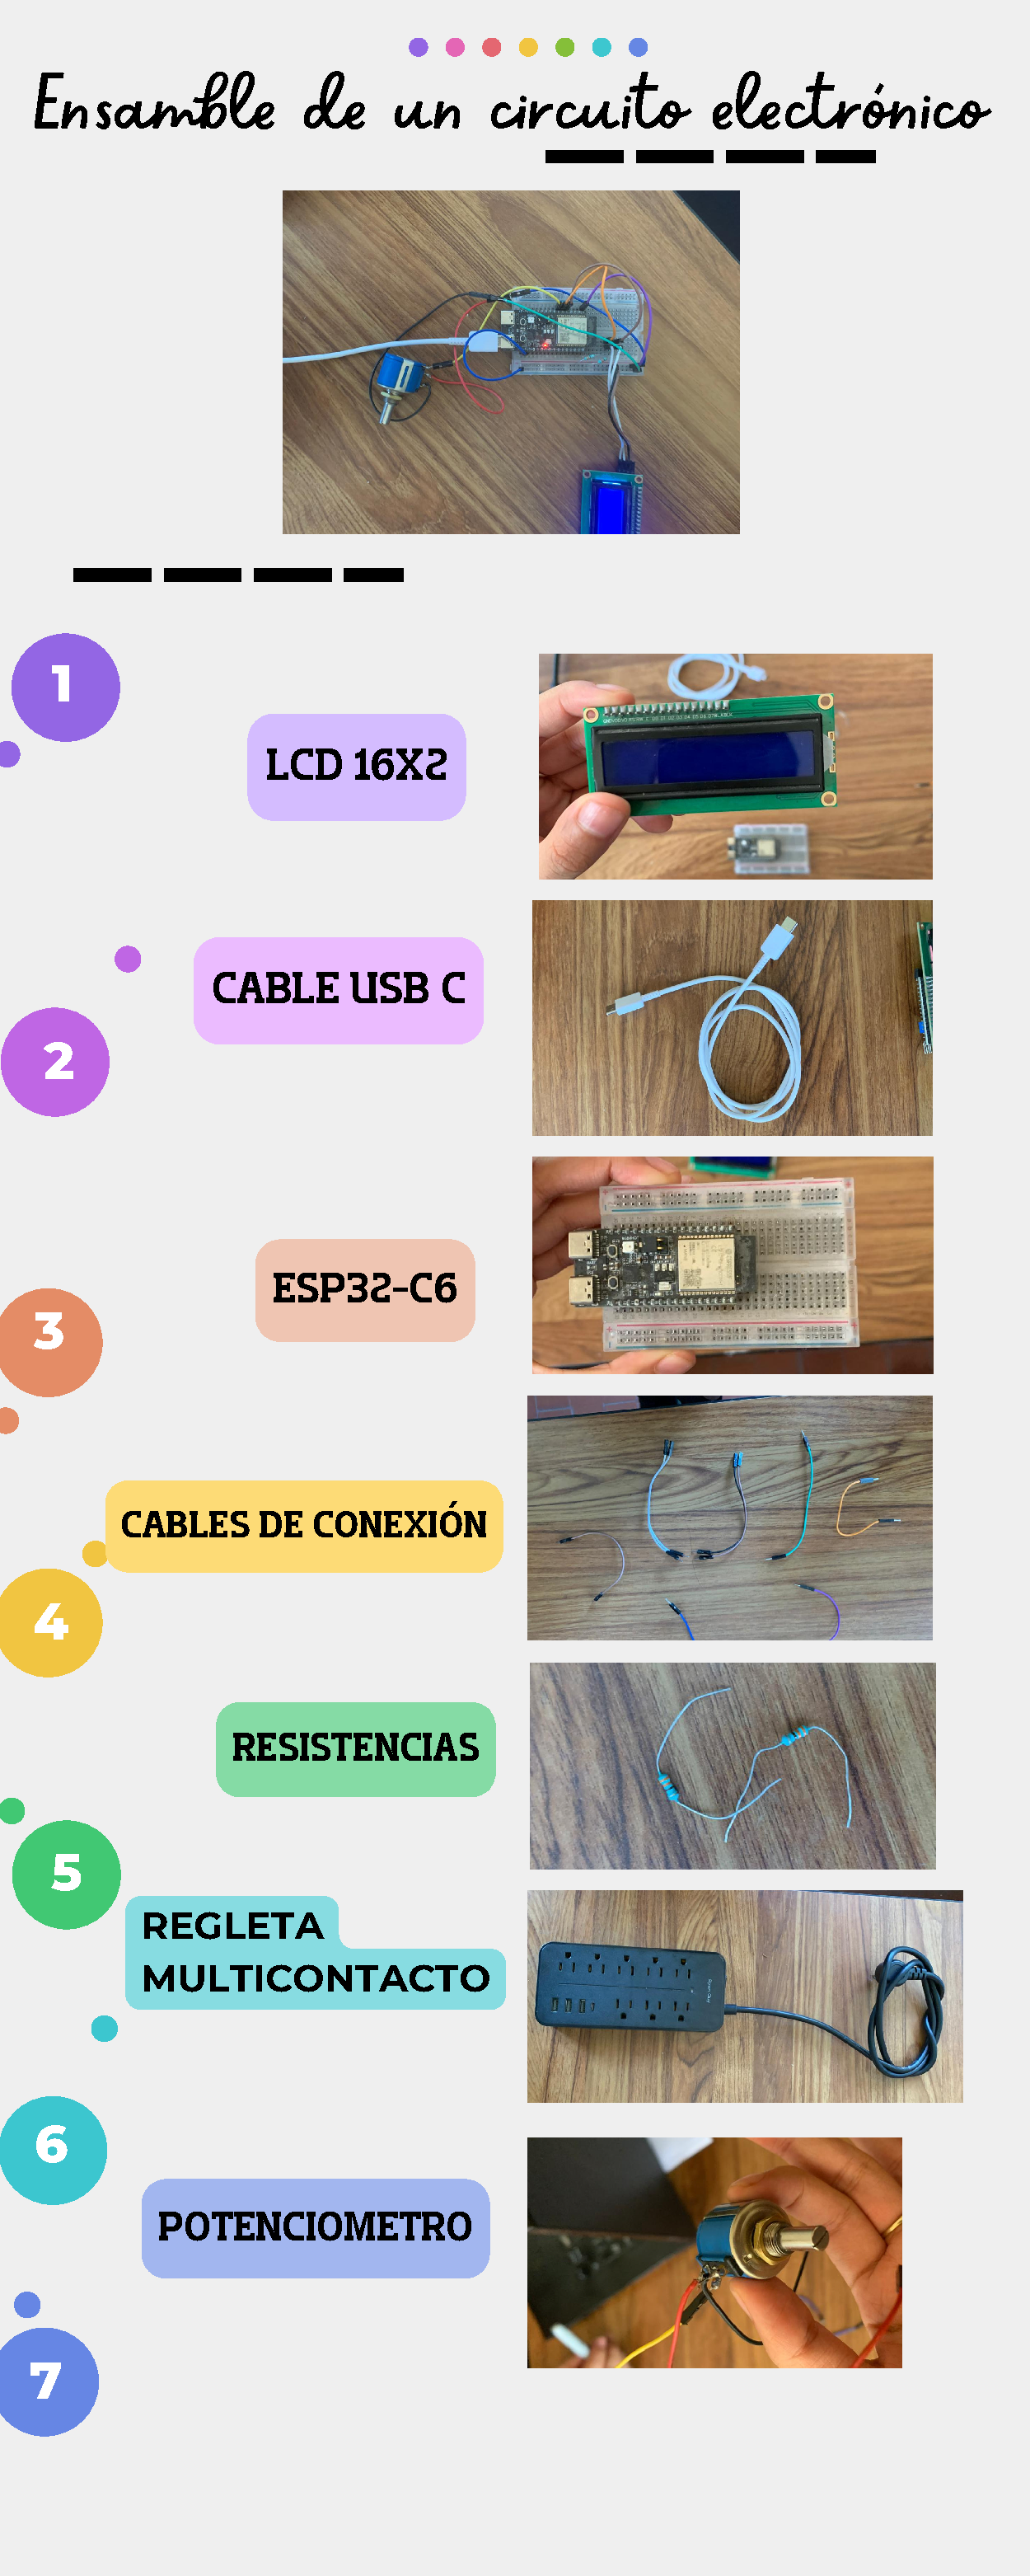
\includepdf[pages=-]{16/Img/materialesCE}
%%%%%%%%%%%%%%%%%%%%%%%%%%%%%%%%%%
%\centering{\section[\appendixautorefname{}]{Apéndice}}\label{anexo:instructivoCE(1)}
%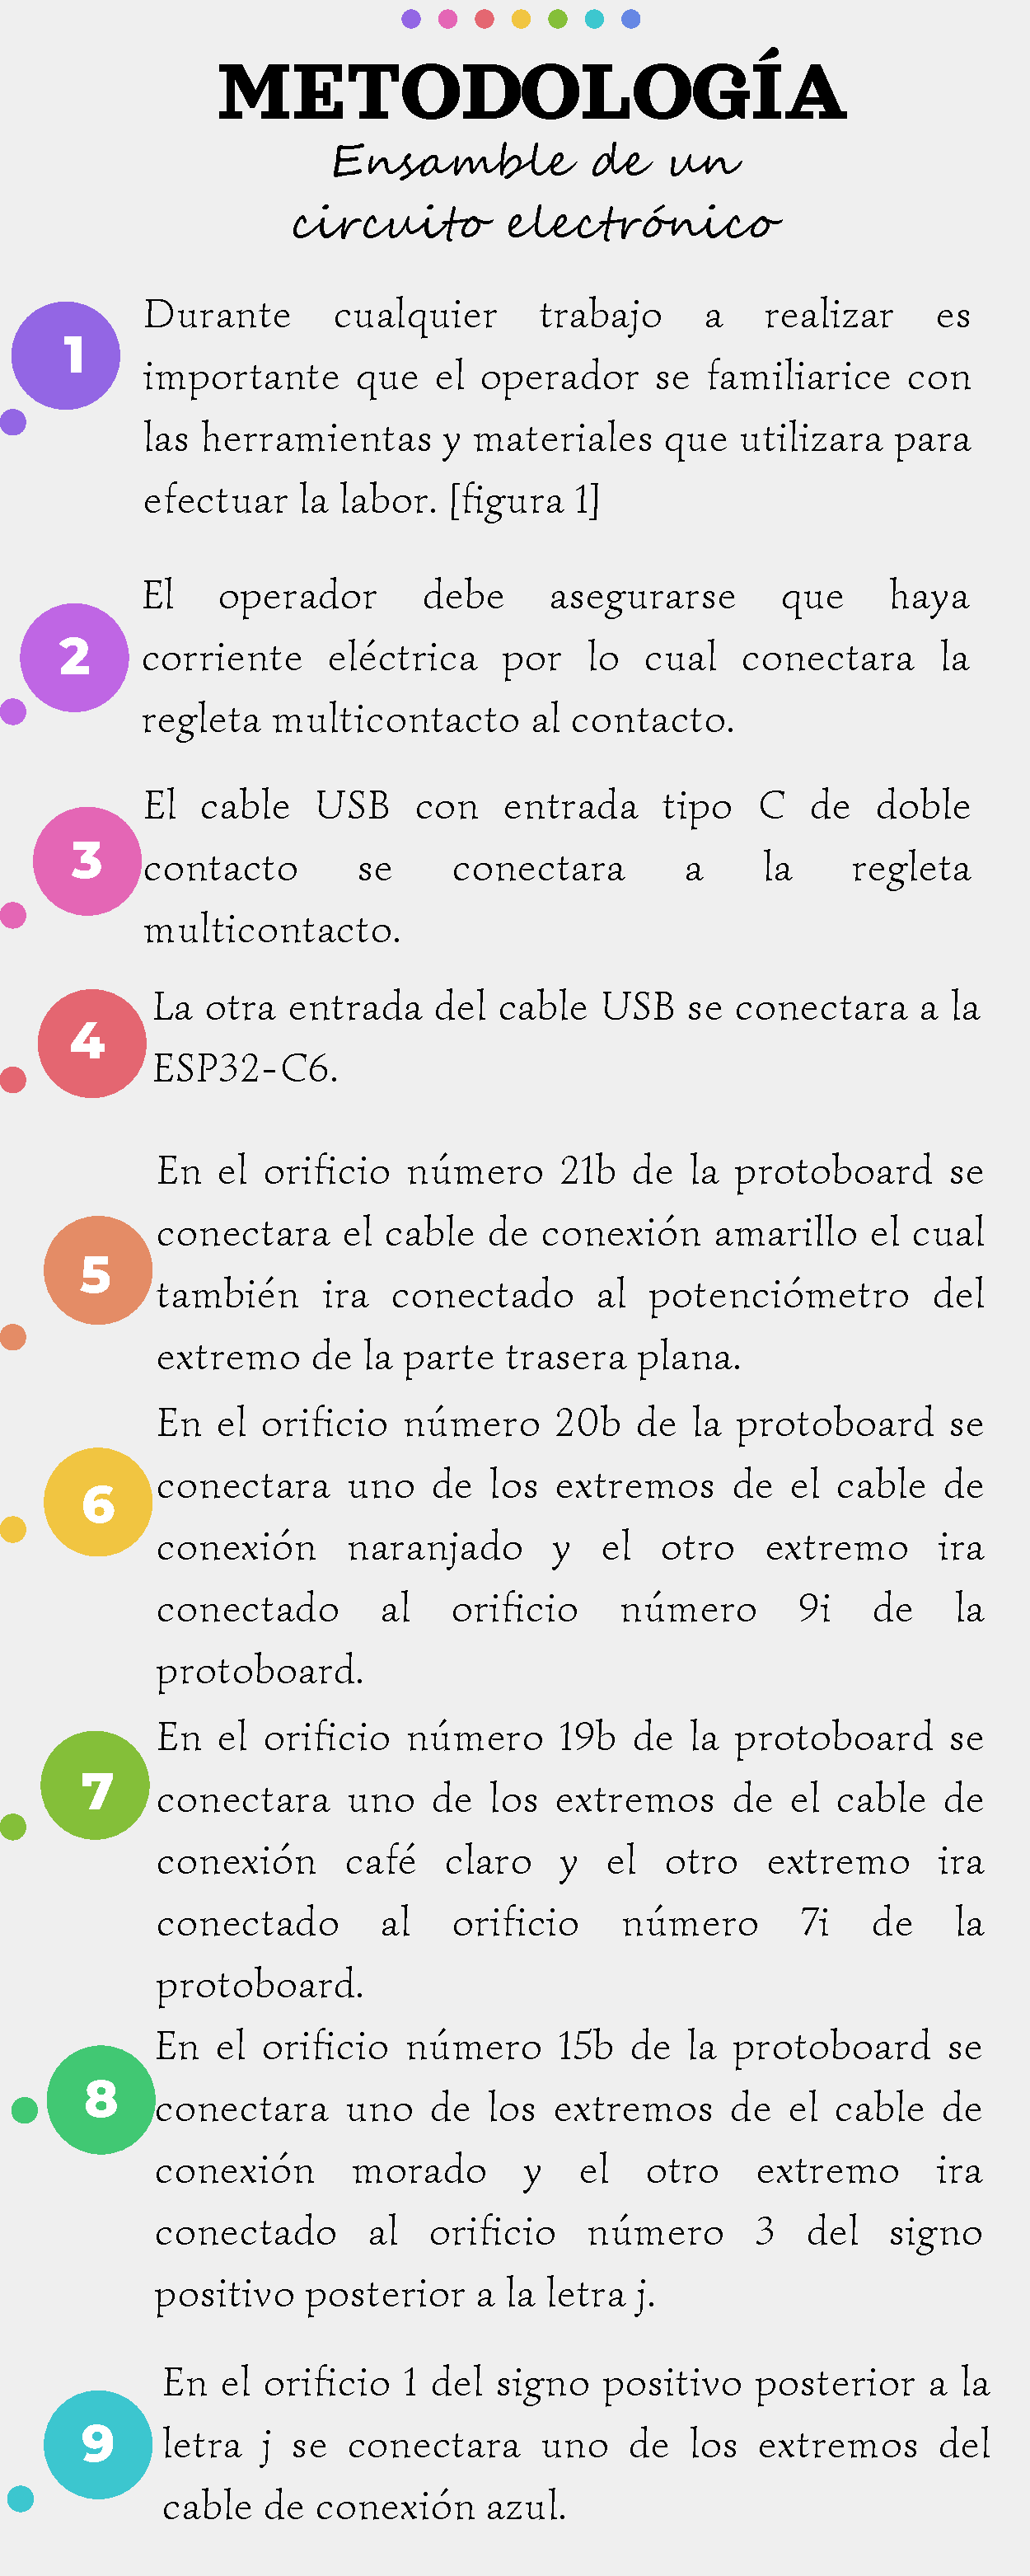
\includepdf[pages=-]{16/Img/instructivoCE(1).pdf}
%%%%%%%%%%%%%%%%%%%%%%%%%%%%%%%%%%
%\centering{\section[\appendixautorefname{}]{Apéndice}}\label{anexo:instructivoCE(2)}
%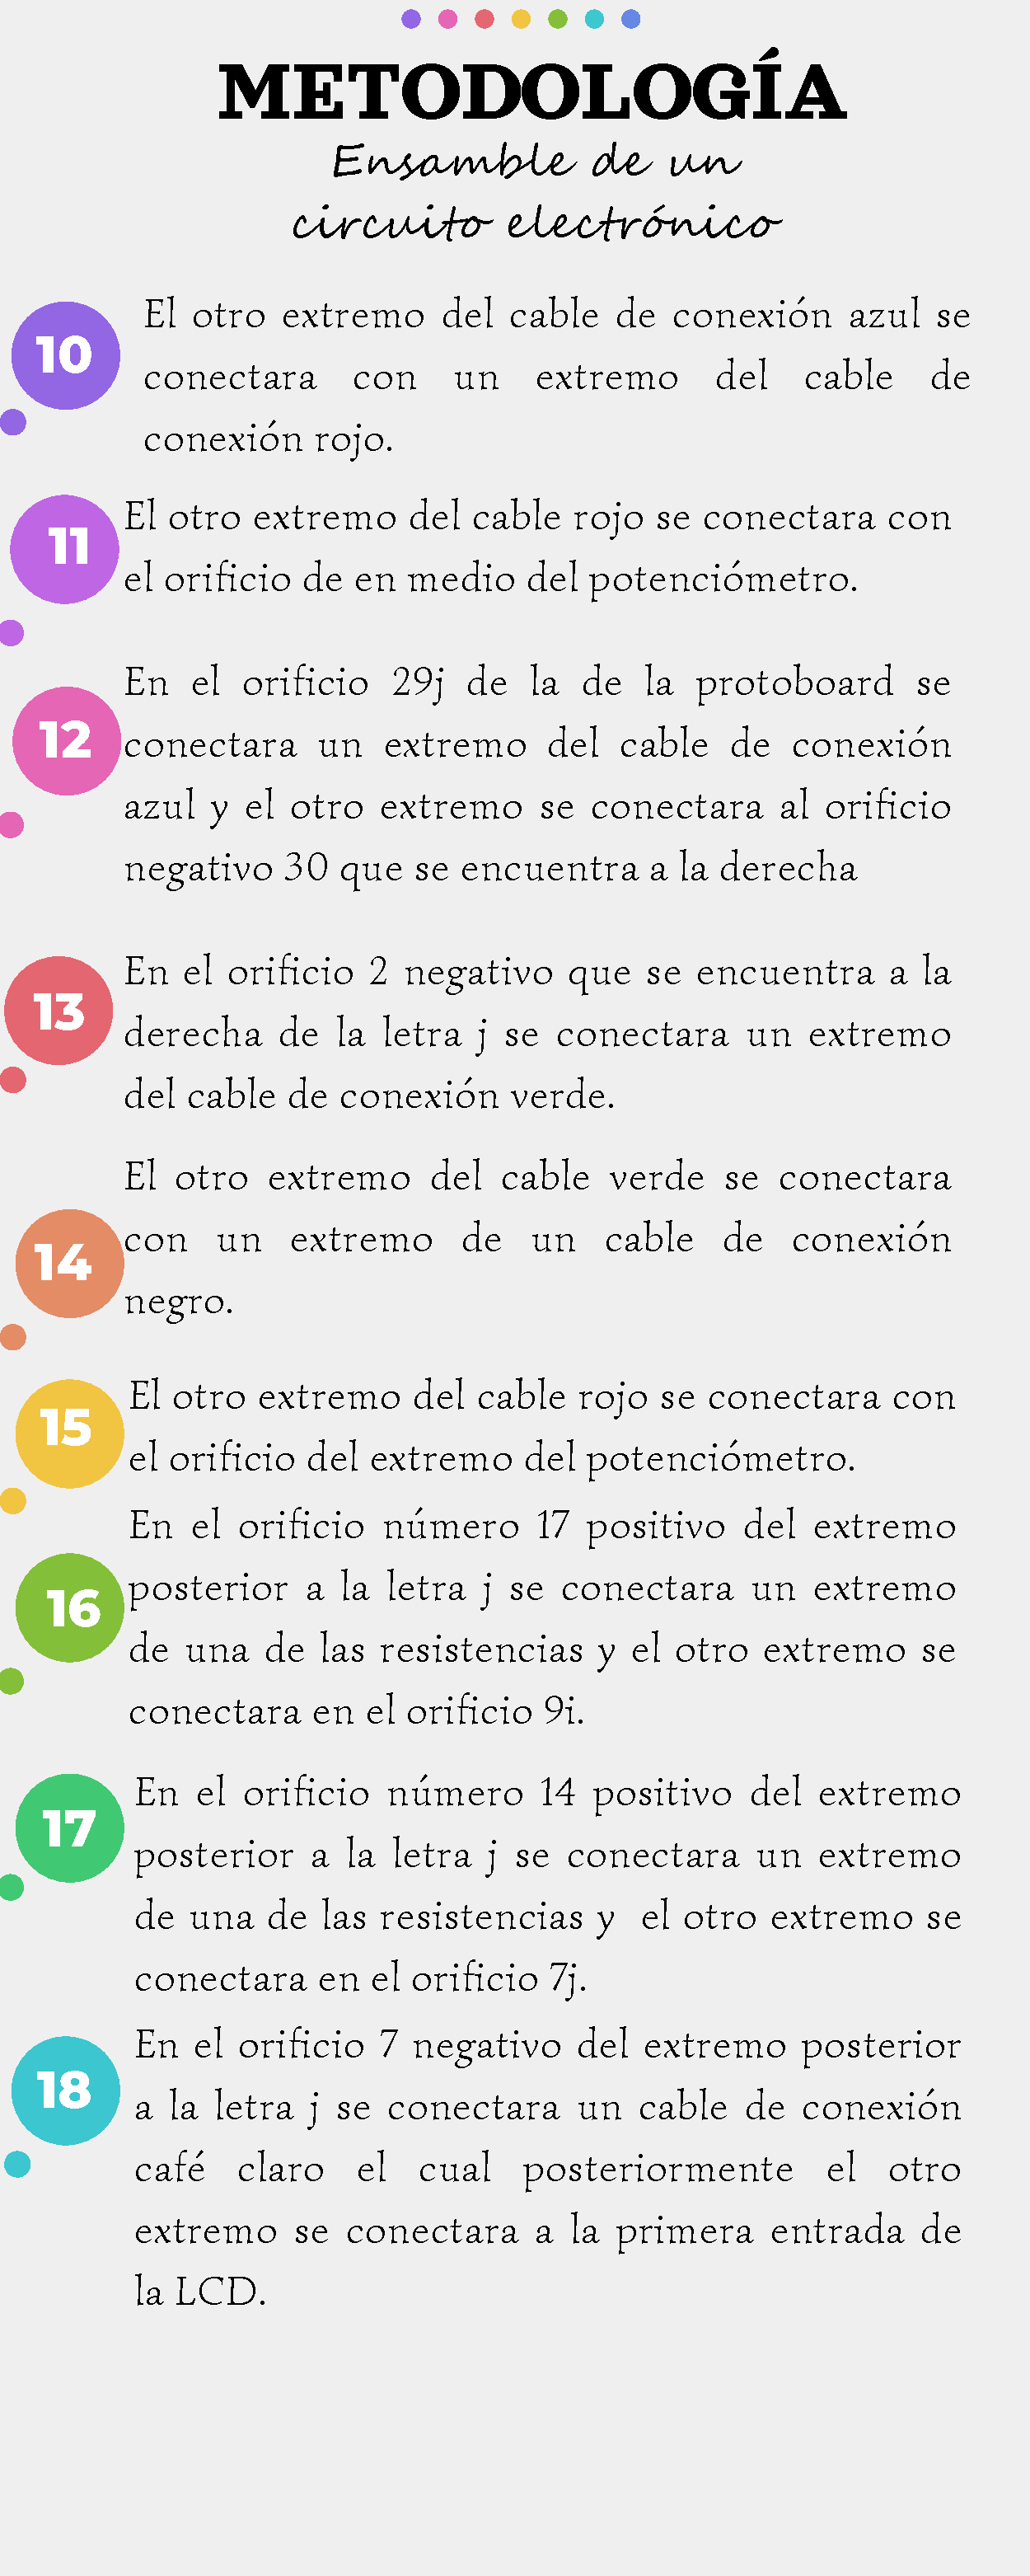
\includepdf[pages=-]{16/Img/instructivoCE(2)}
%%%%%%%%%%%%%%%%%%%%%%%%%%%%%%%%%%
%\centering{\section[\appendixautorefname{}]{Apéndice}}\label{anexo:instructivoCE(3)}
%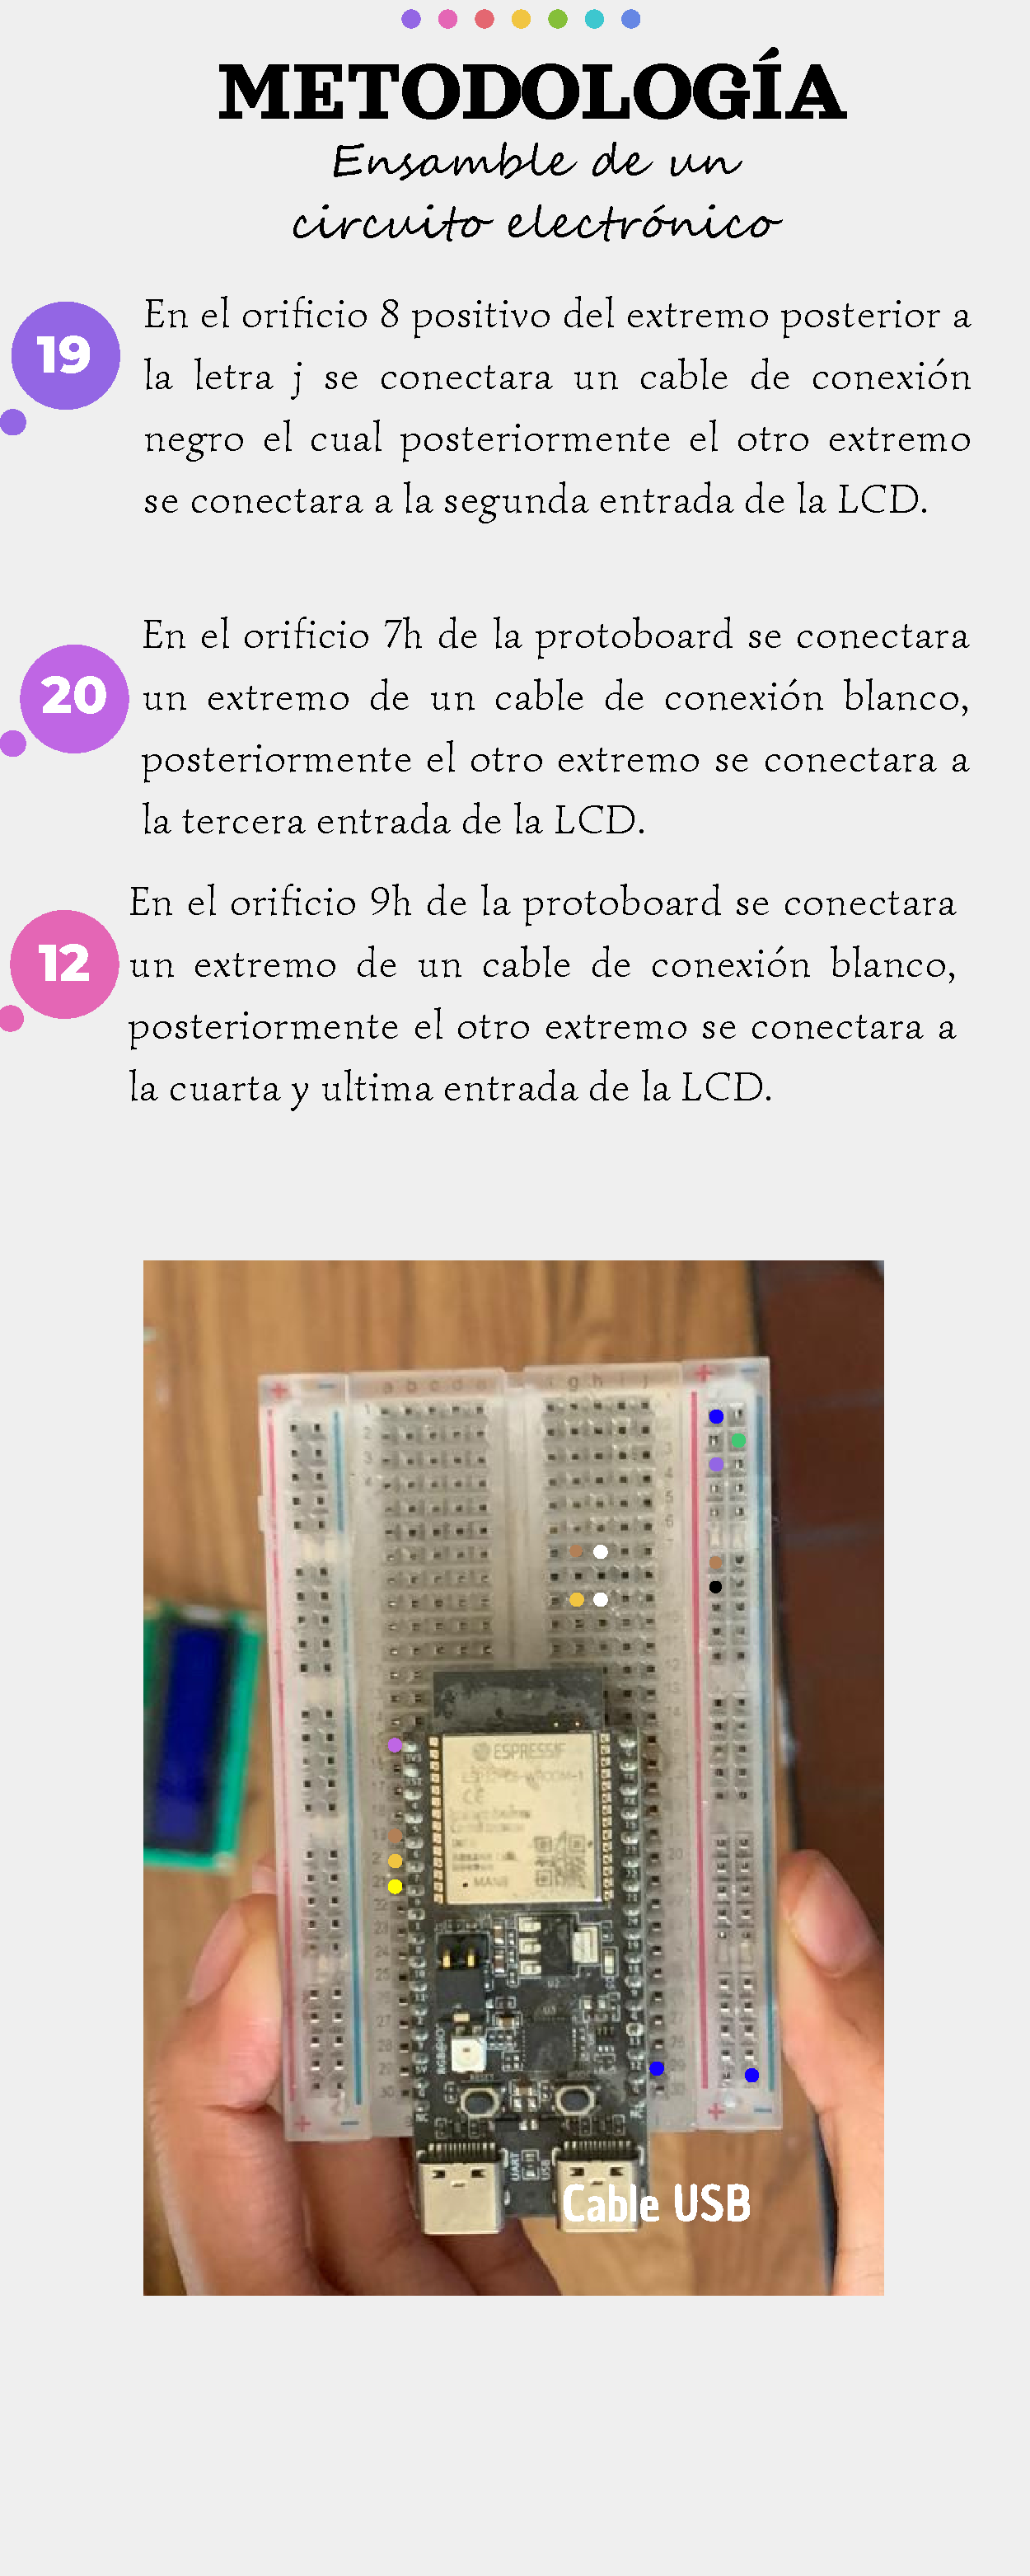
\includepdf[pages=-]{16/Img/instructivoCE(3)}
%%%%%%%%%%%%%%%%%%%%%%%%%%%%%%%%%%
%\centering{\section[\appendixautorefname{}]{Apéndice}}\label{anexo:instructivoCE(4)}
%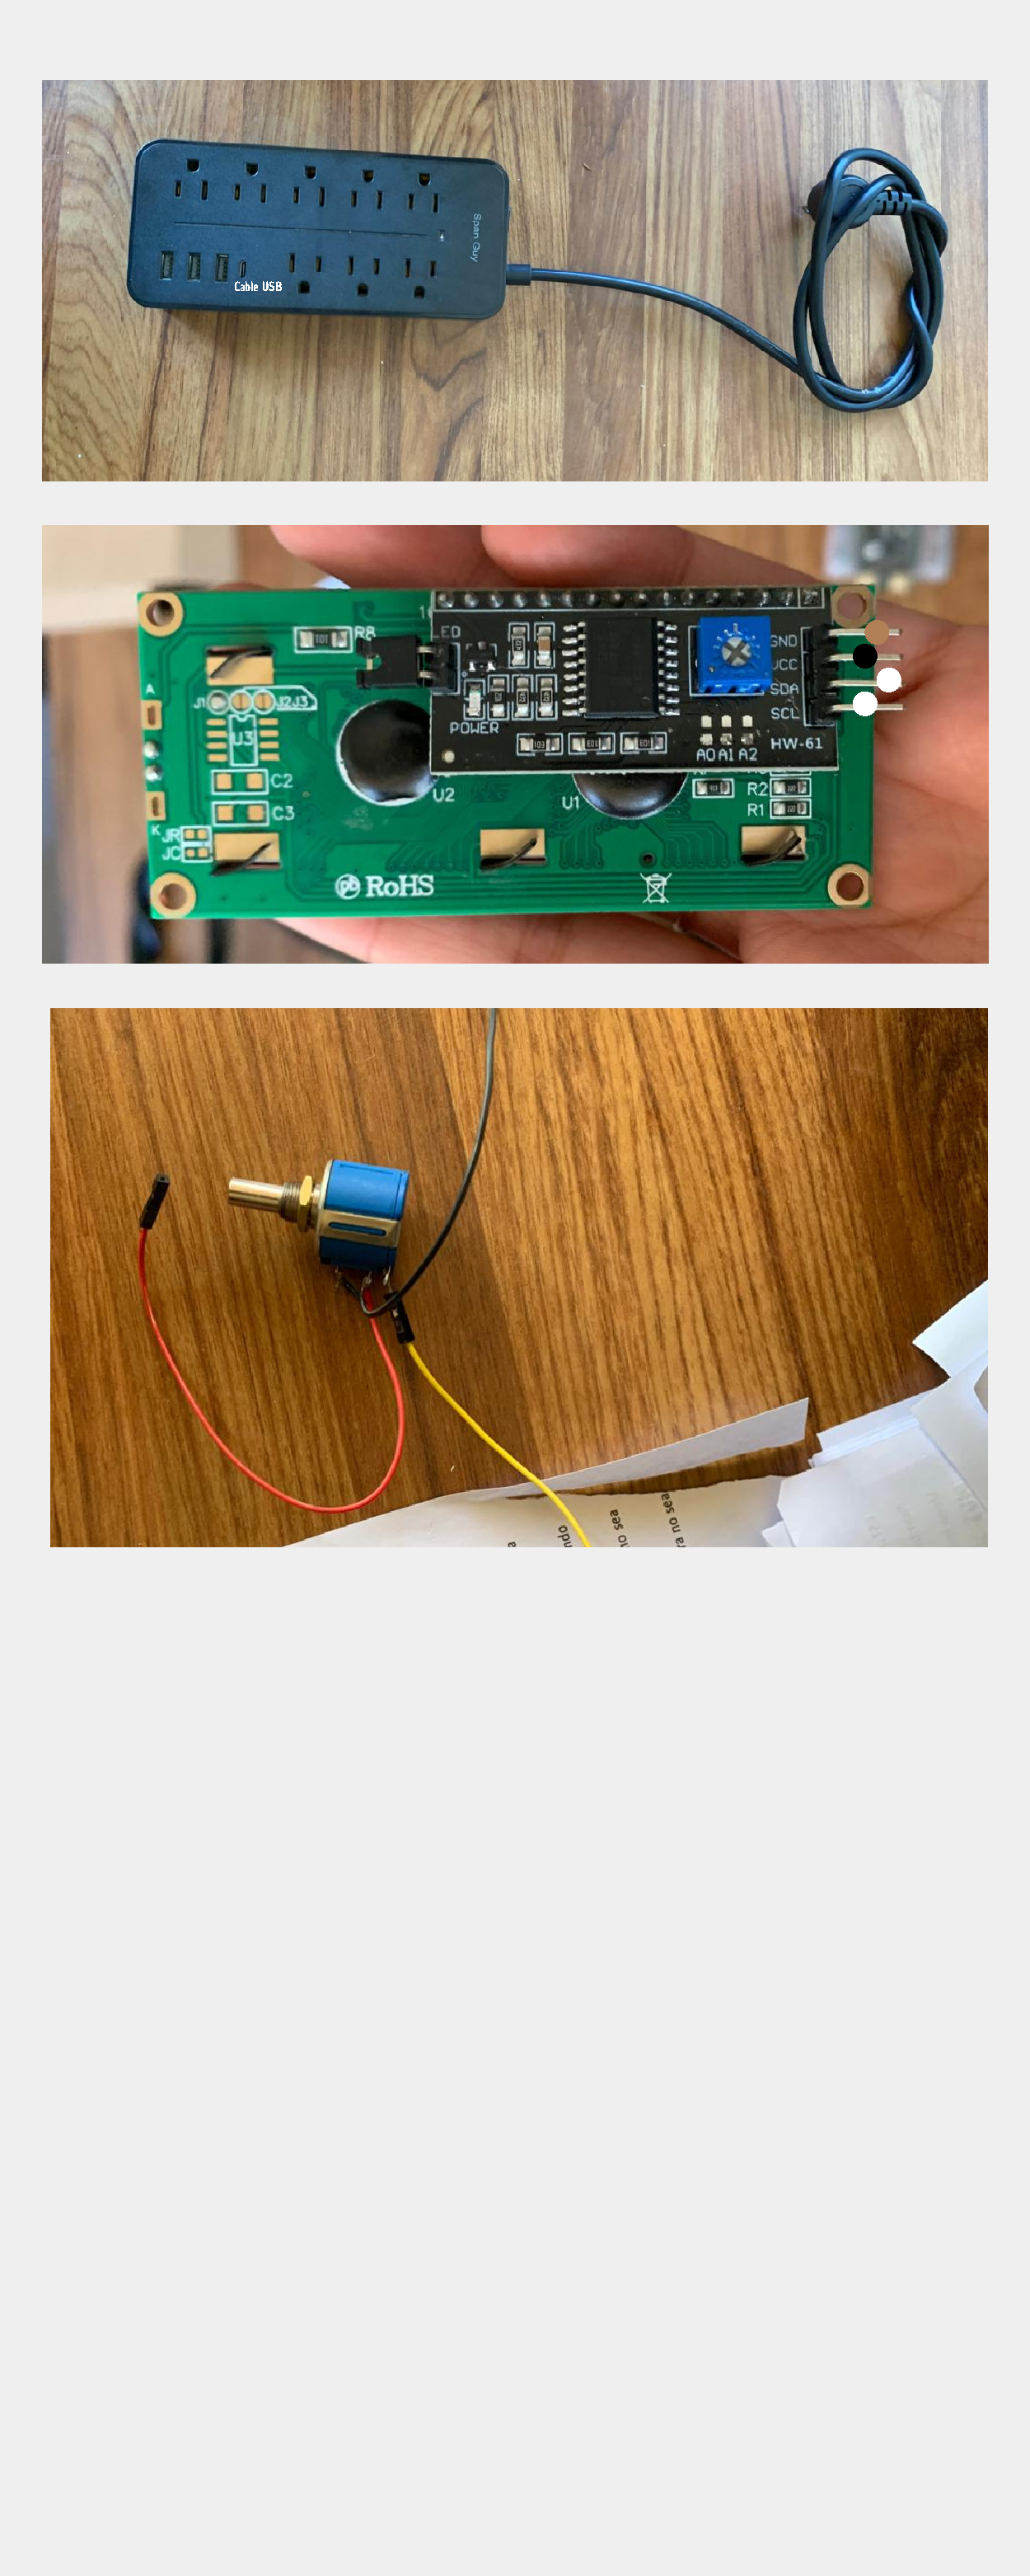
\includepdf[pages=-]{16/Img/instructivoCE(4)}
%%%%%%%%%%%%%%%%%%%%%%%%%%%%%%%%%%
%\centering{\section[\appendixautorefname{}]{Apéndice}}\label{anexo:cablesDeConexión}
%\includepdf[pages=-]{16/Img/cablesDeConexión}
%%%%%%%%%%%%%%%%%%%%%%%%%%%%%%%%%%
%\centering{\section[\appendixautorefname{}]{Apéndice}}\label{anexo:cableUSB}
%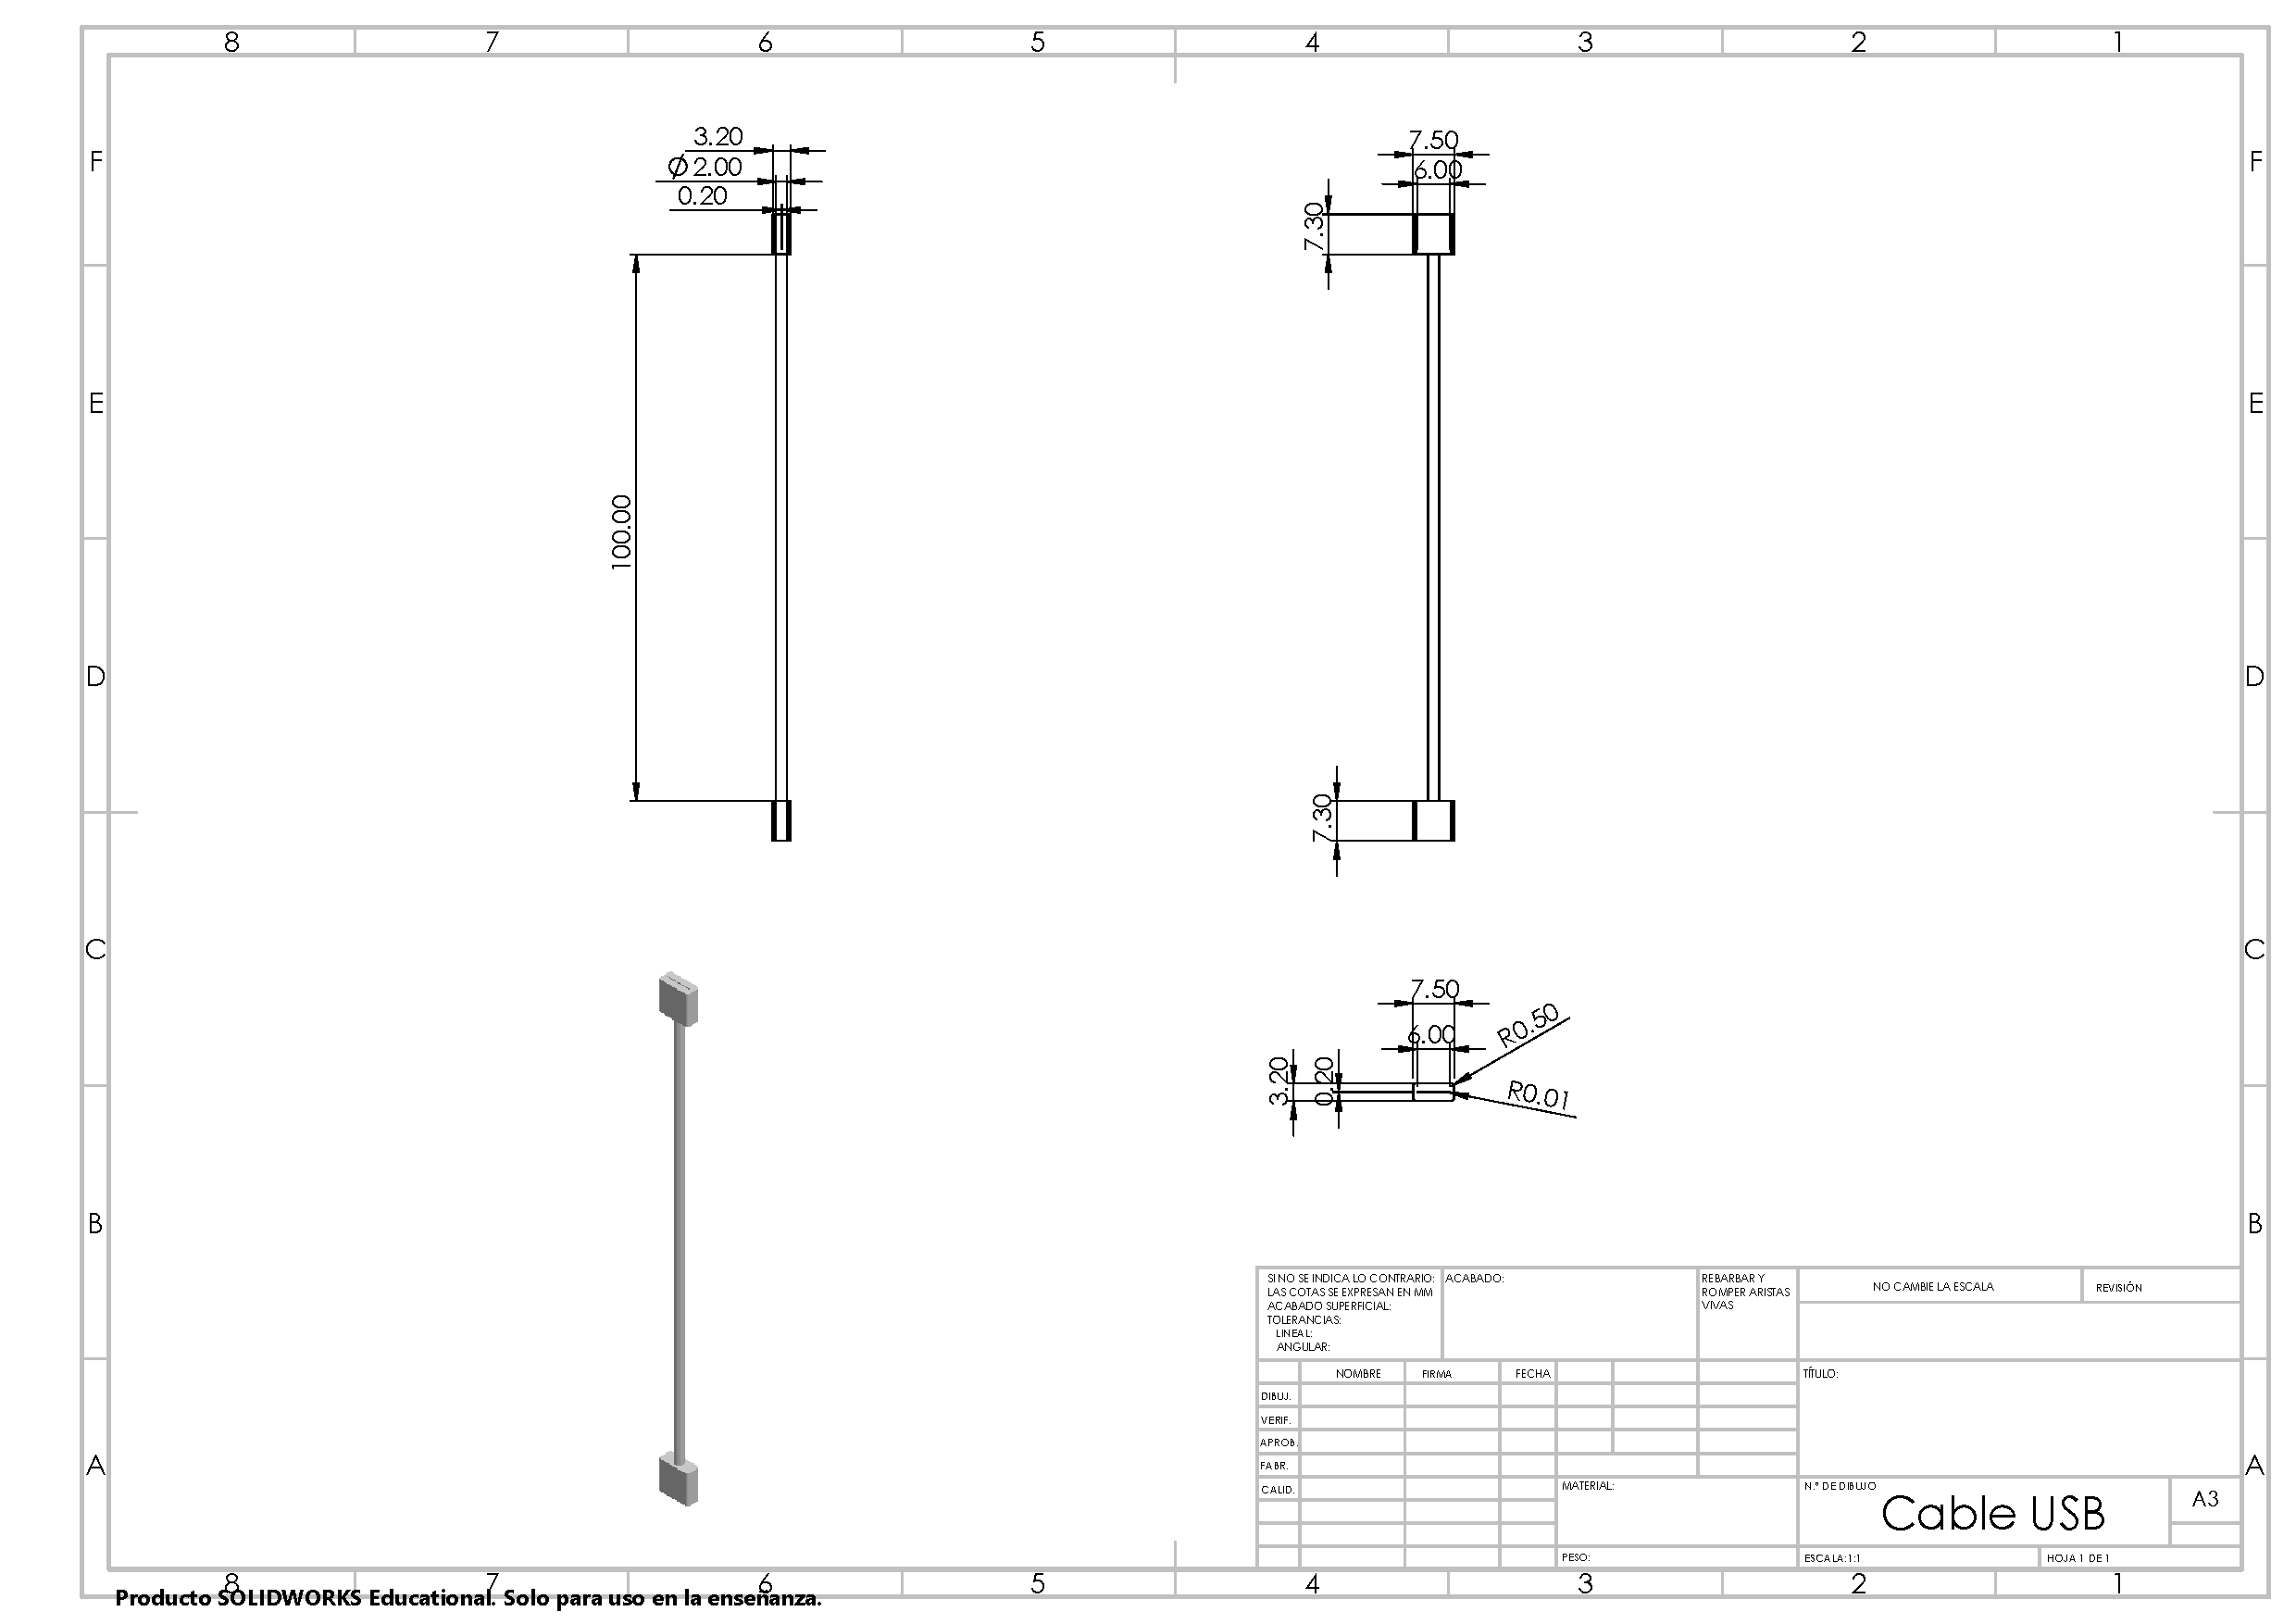
\includepdf[pages=-]{16/Img/cableUSB}
%%%%%%%%%%%%%%%%%%%%%%%%%%%%%%%%%%
%\centering{\section[\appendixautorefname{}]{Apéndice}}\label{anexo:eSP32}
%\includepdf[pages=-]{16/Img/eSP32}
%%%%%%%%%%%%%%%%%%%%%%%%%%%%%%%%%%
%\centering{\section[\appendixautorefname{}]{Apéndice}}\label{anexo:lCD16X2}
%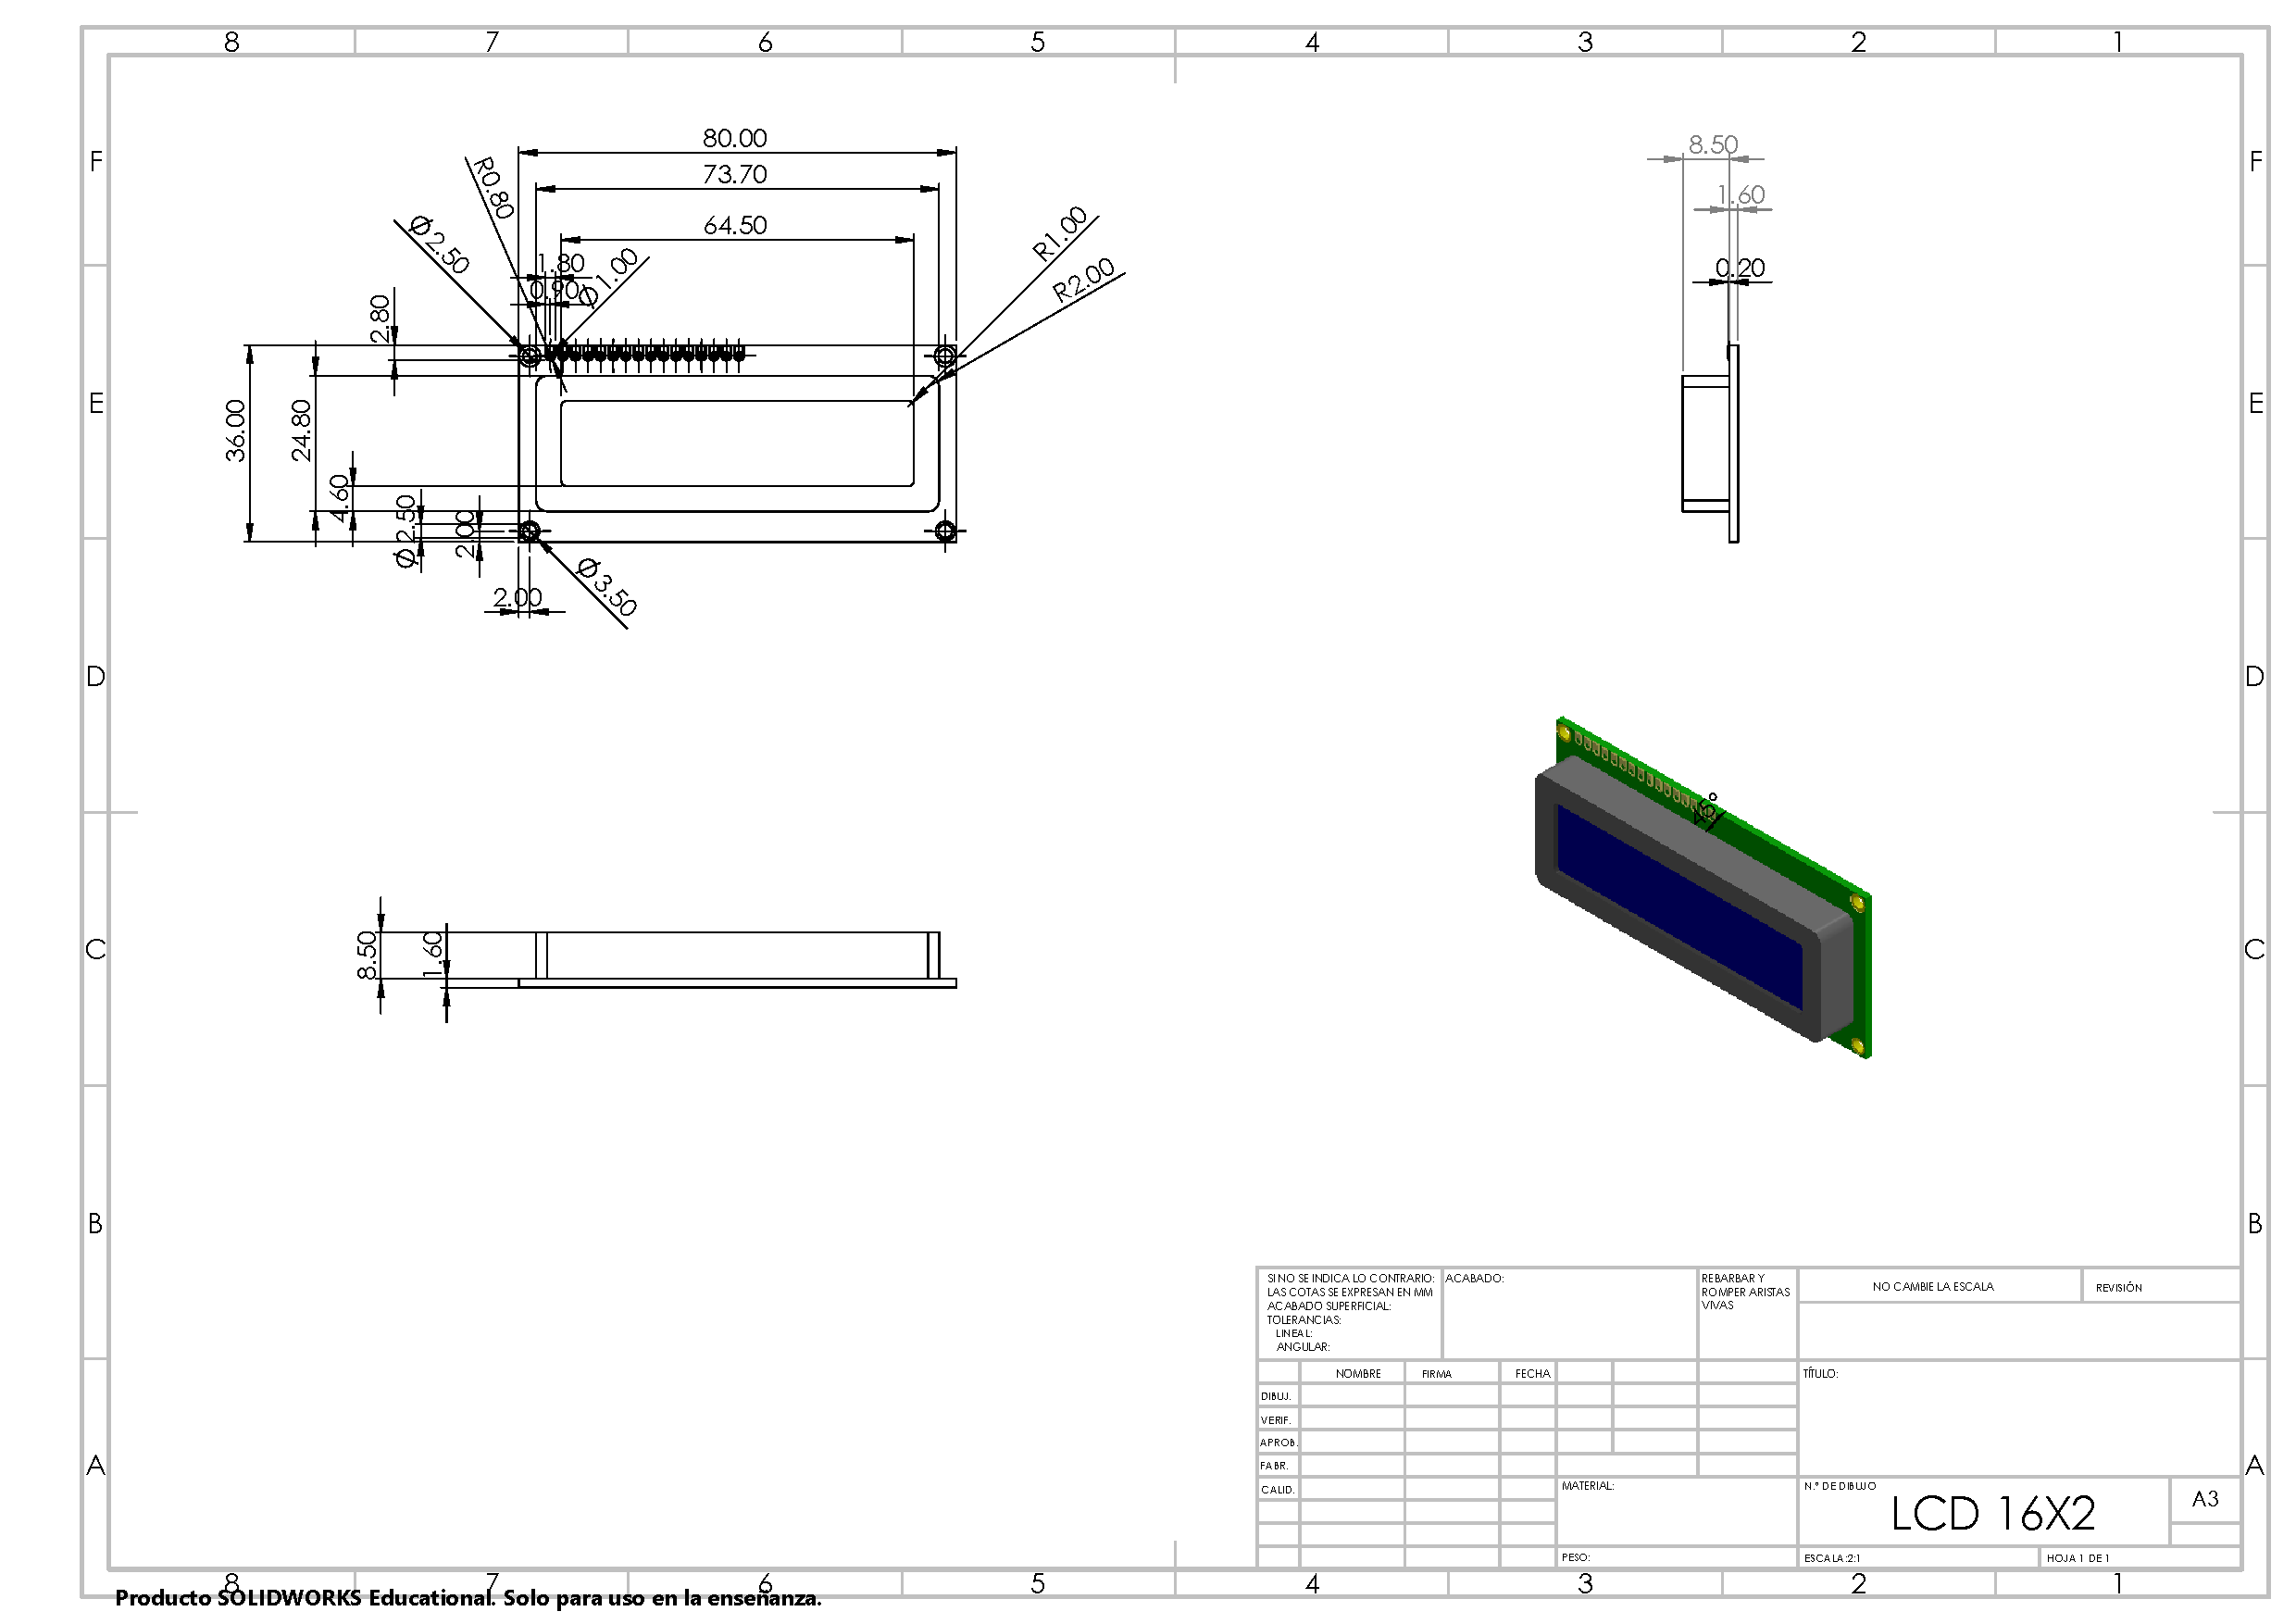
\includepdf[pages=-]{16/Img/lCD16X2}
%%%%%%%%%%%%%%%%%%%%%%%%%%%%%%%%%%
%\centering{\section[\appendixautorefname{}]{Apéndice}}\label{anexo:modulo12C}
%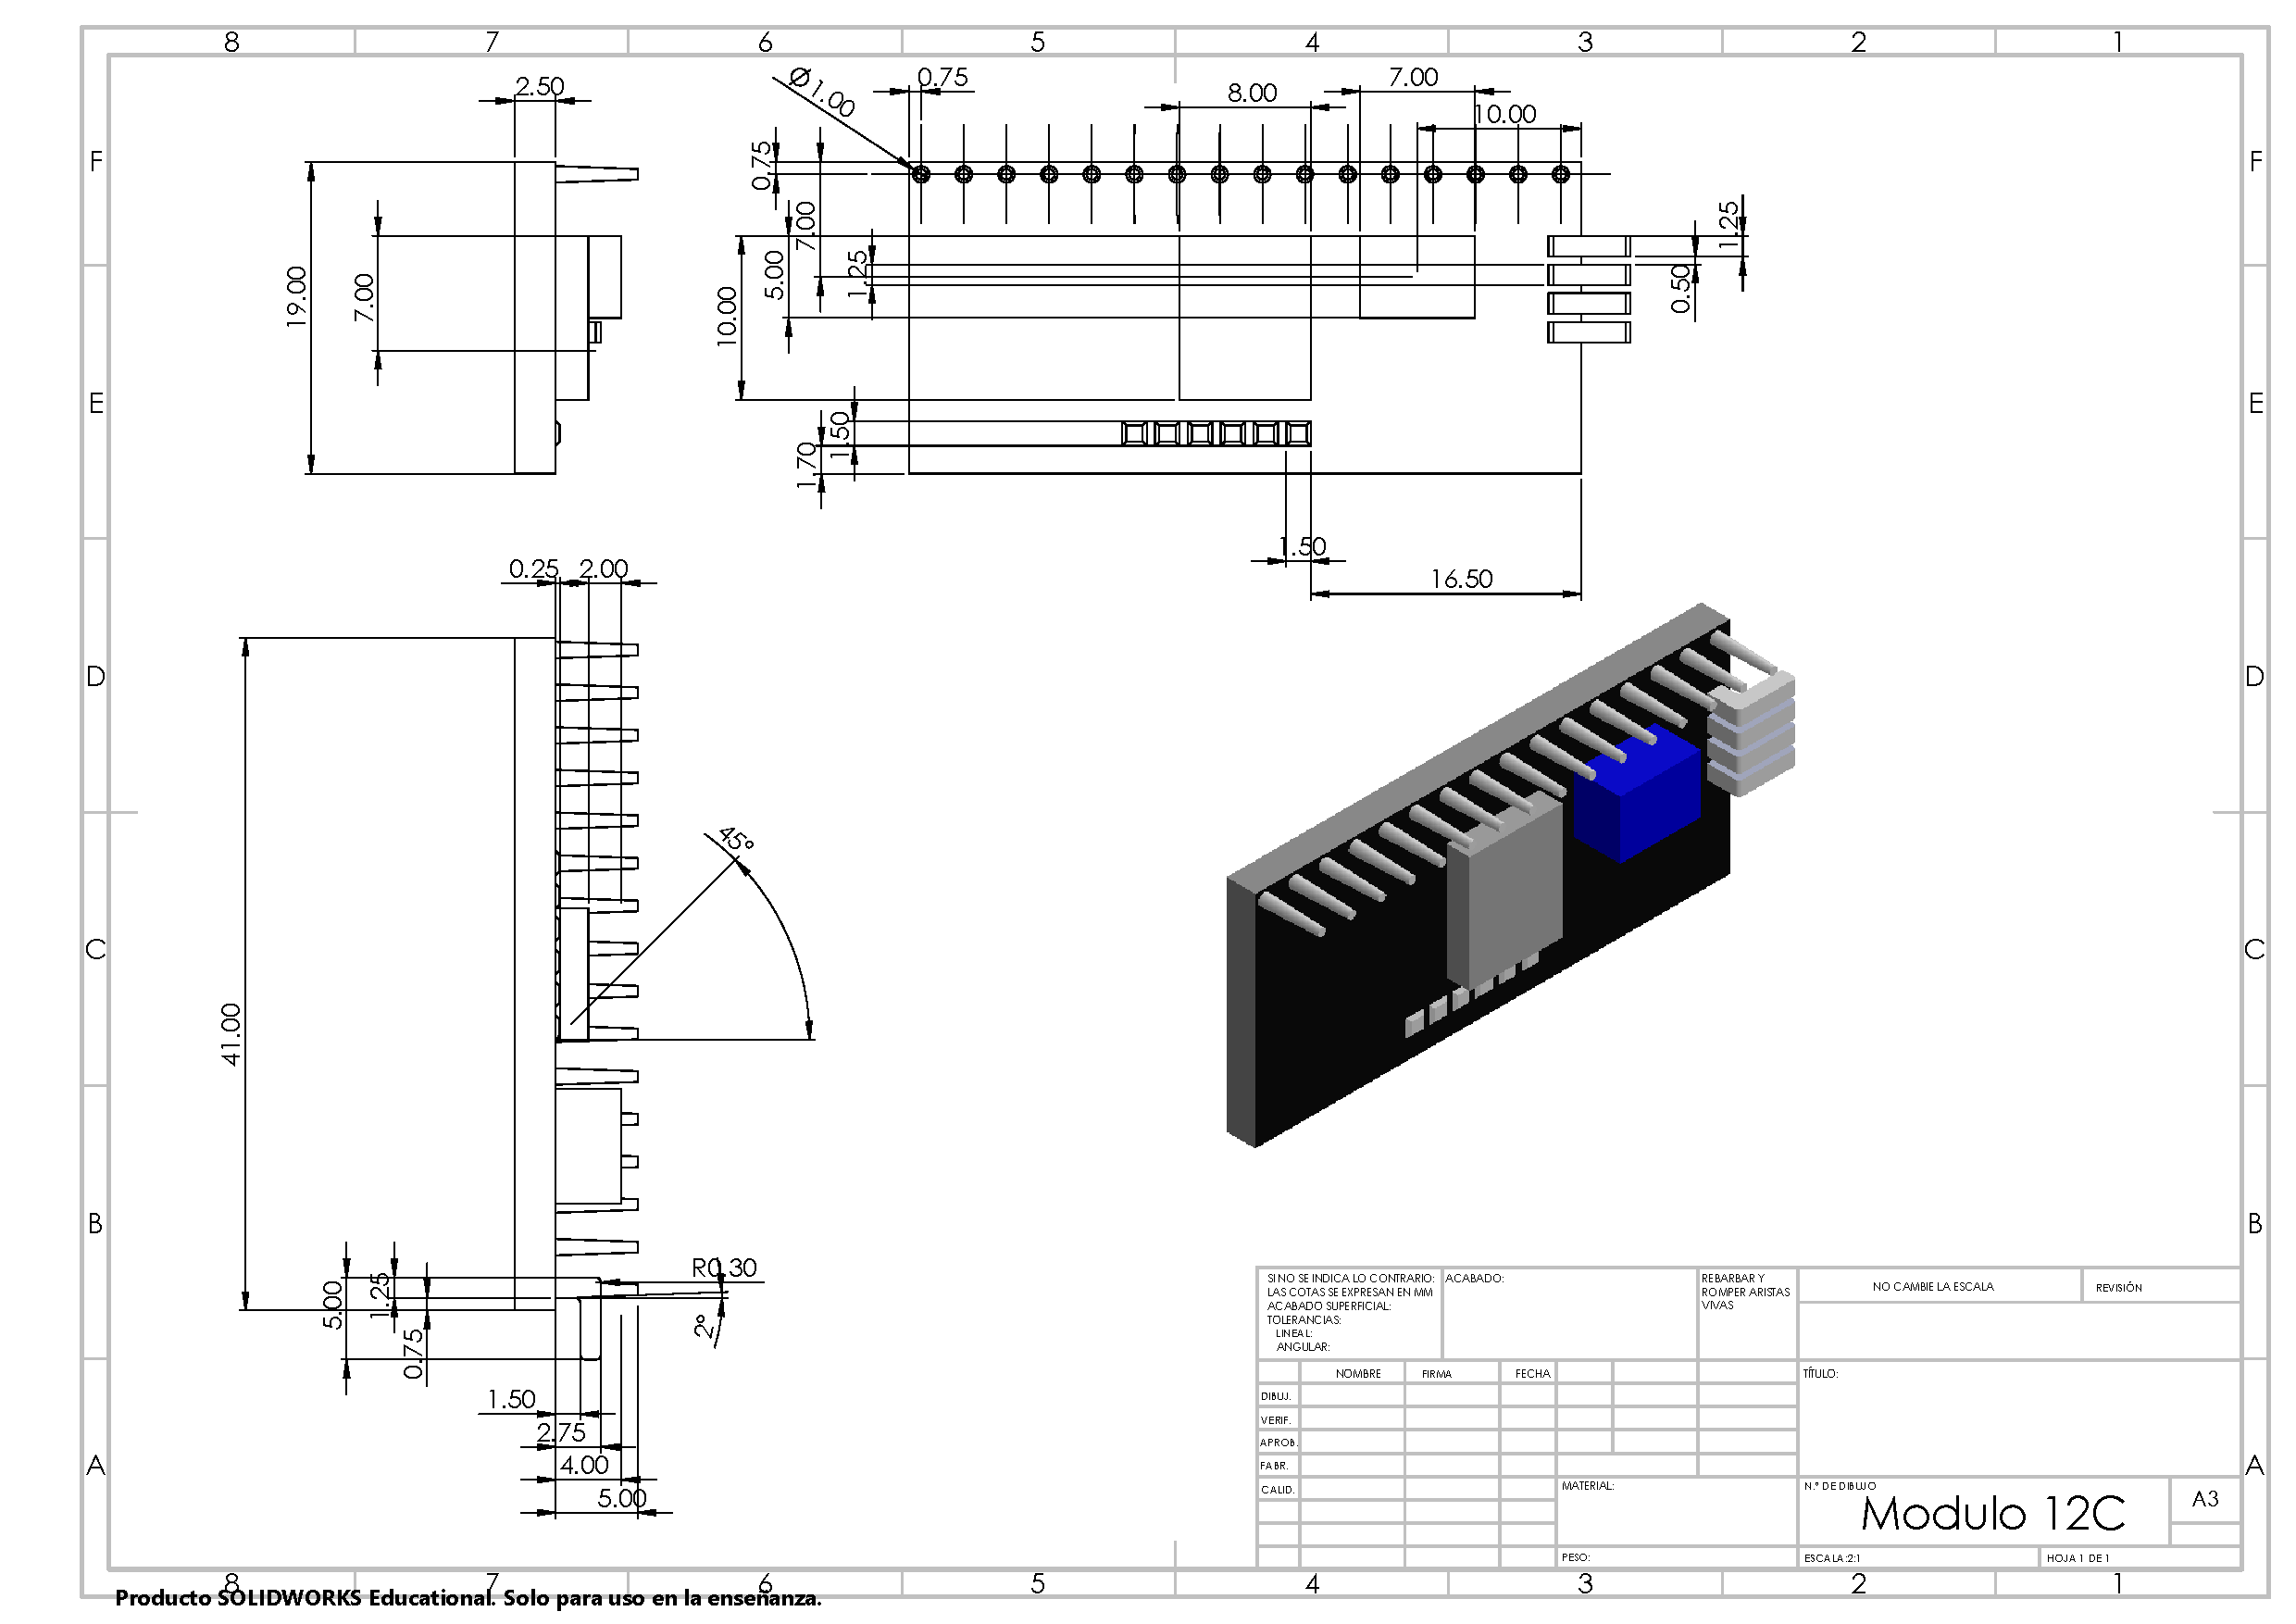
\includepdf[pages=-]{16/Img/modulo12C}
%%%%%%%%%%%%%%%%%%%%%%%%%%%%%%%%%%
%\centering{\section[\appendixautorefname{}]{Apéndice}}\label{anexo:potenciometro}
%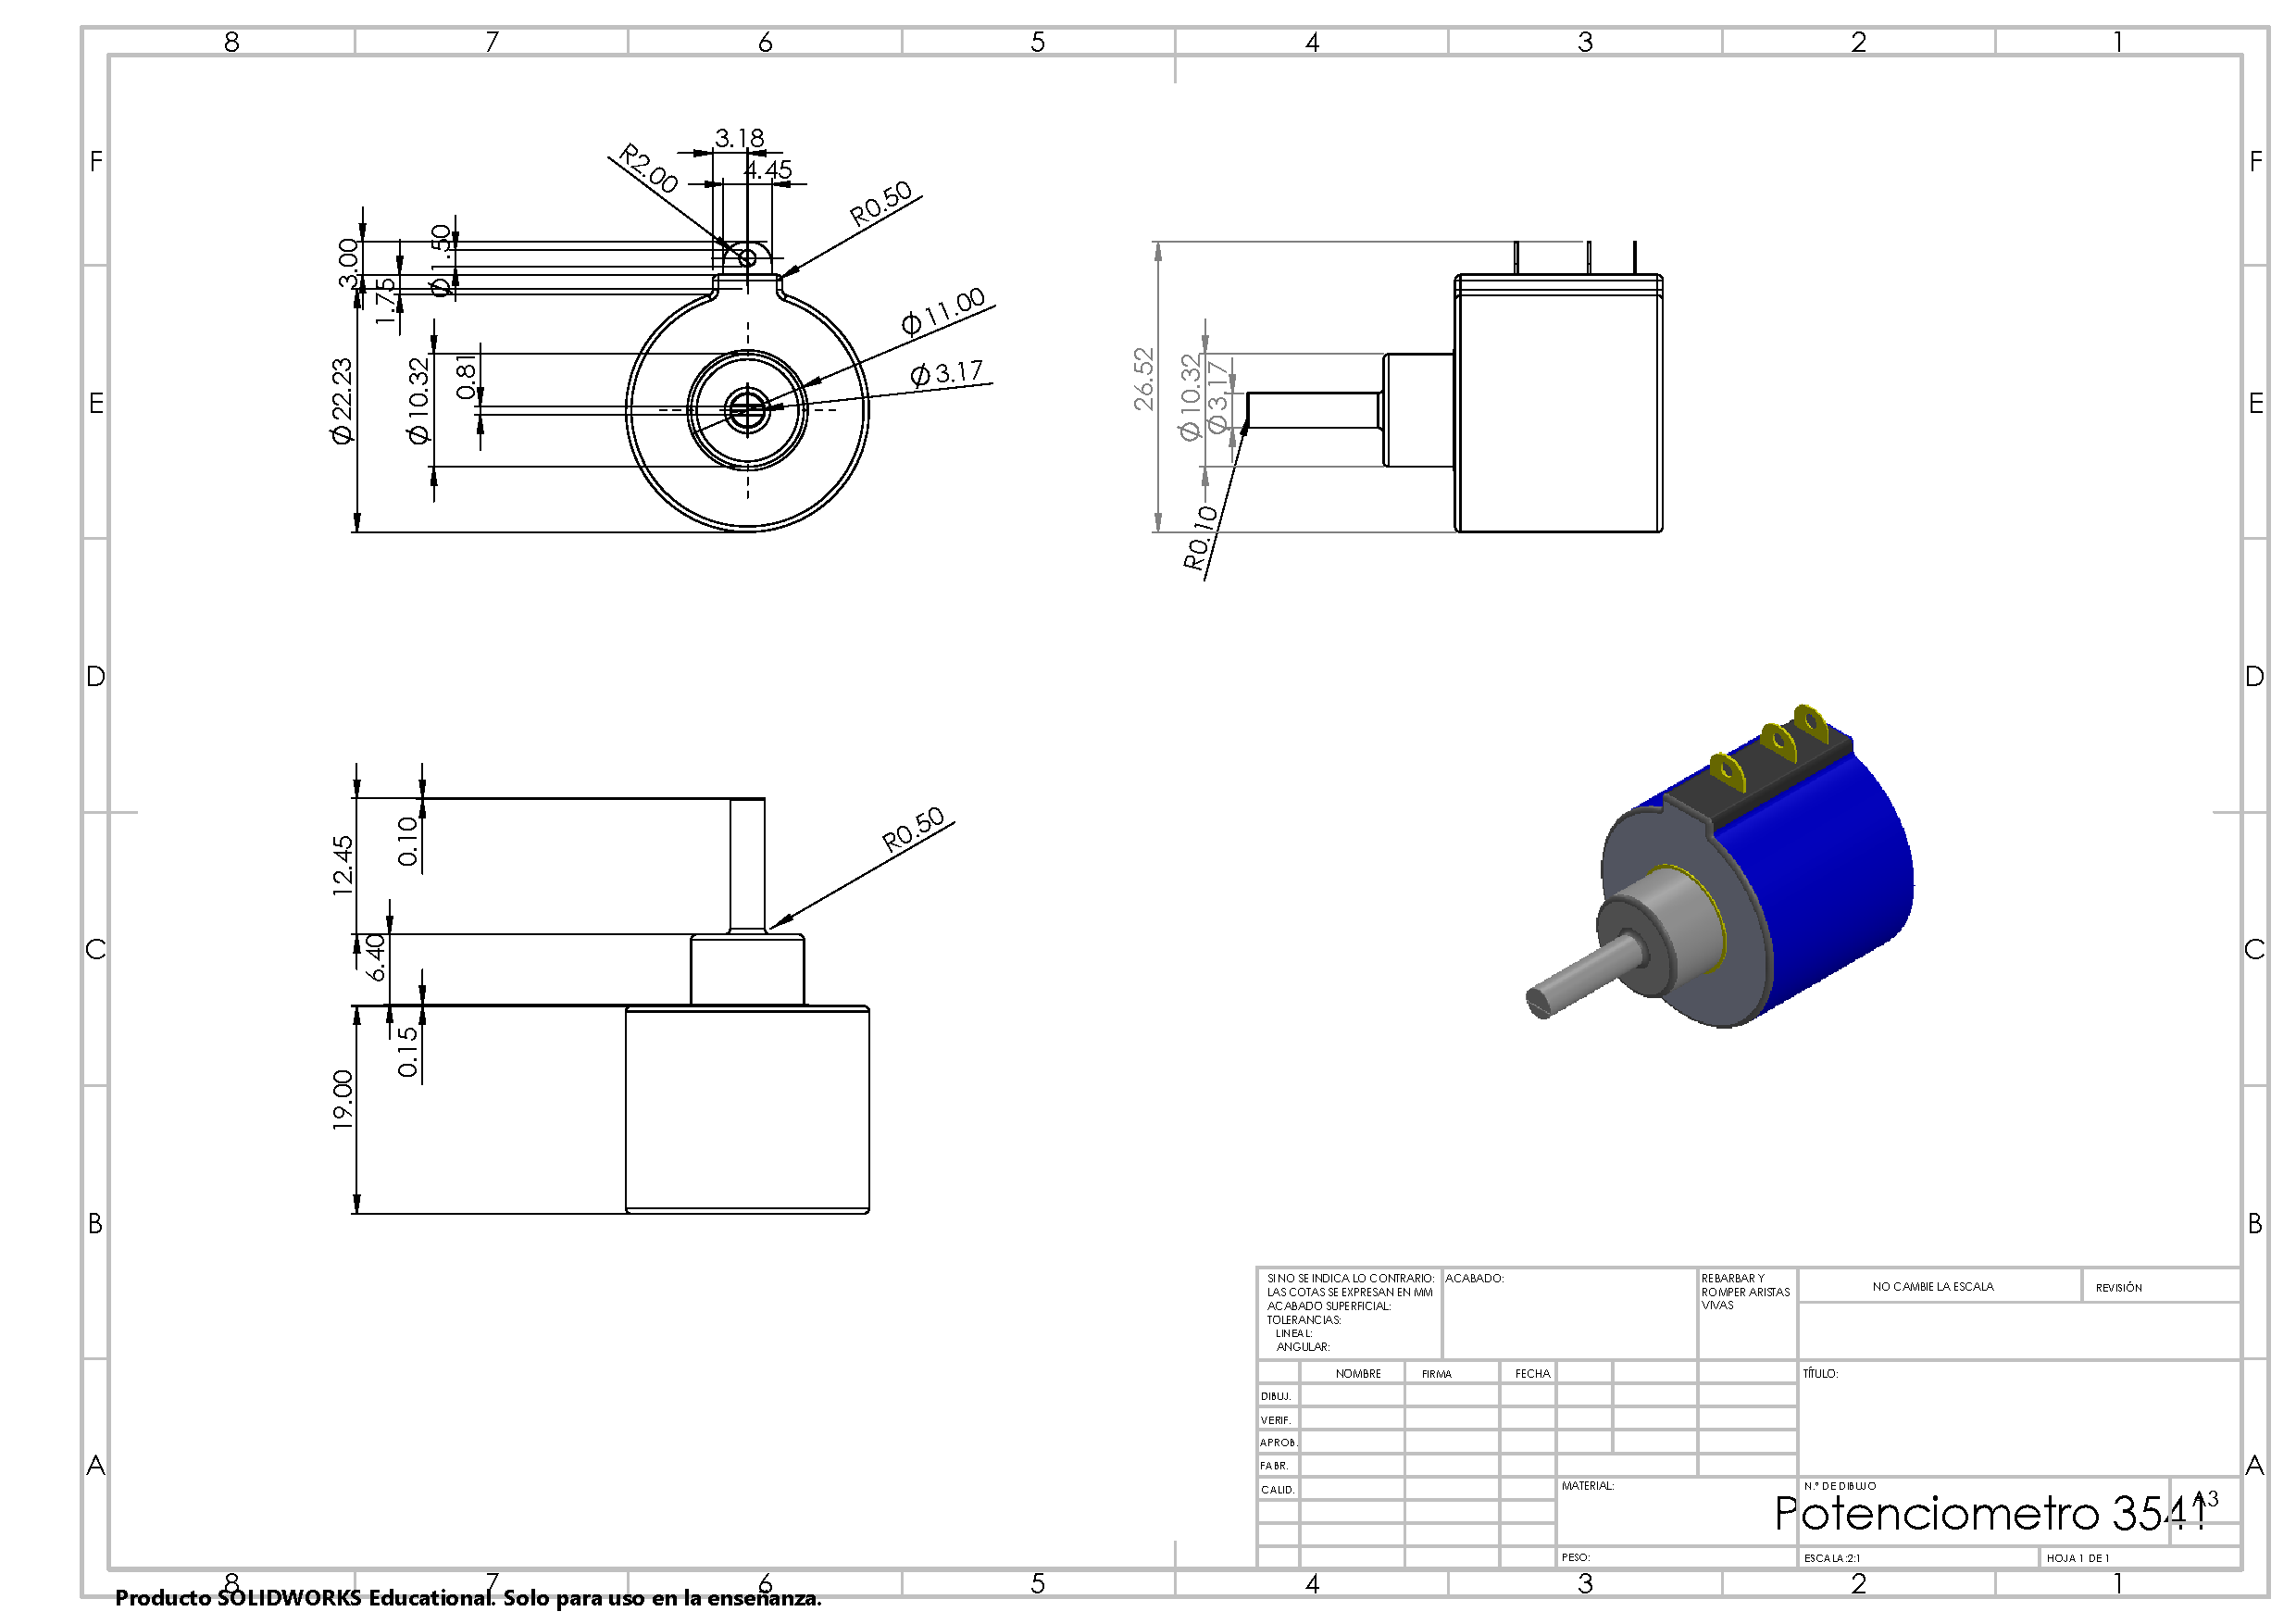
\includepdf[pages=-]{16/Img/potenciometro}
%%%%%%%%%%%%%%%%%%%%%%%%%%%%%%%%%%
%\centering{\section[\appendixautorefname{}]{Apéndice}}\label{anexo:resistencia330}
%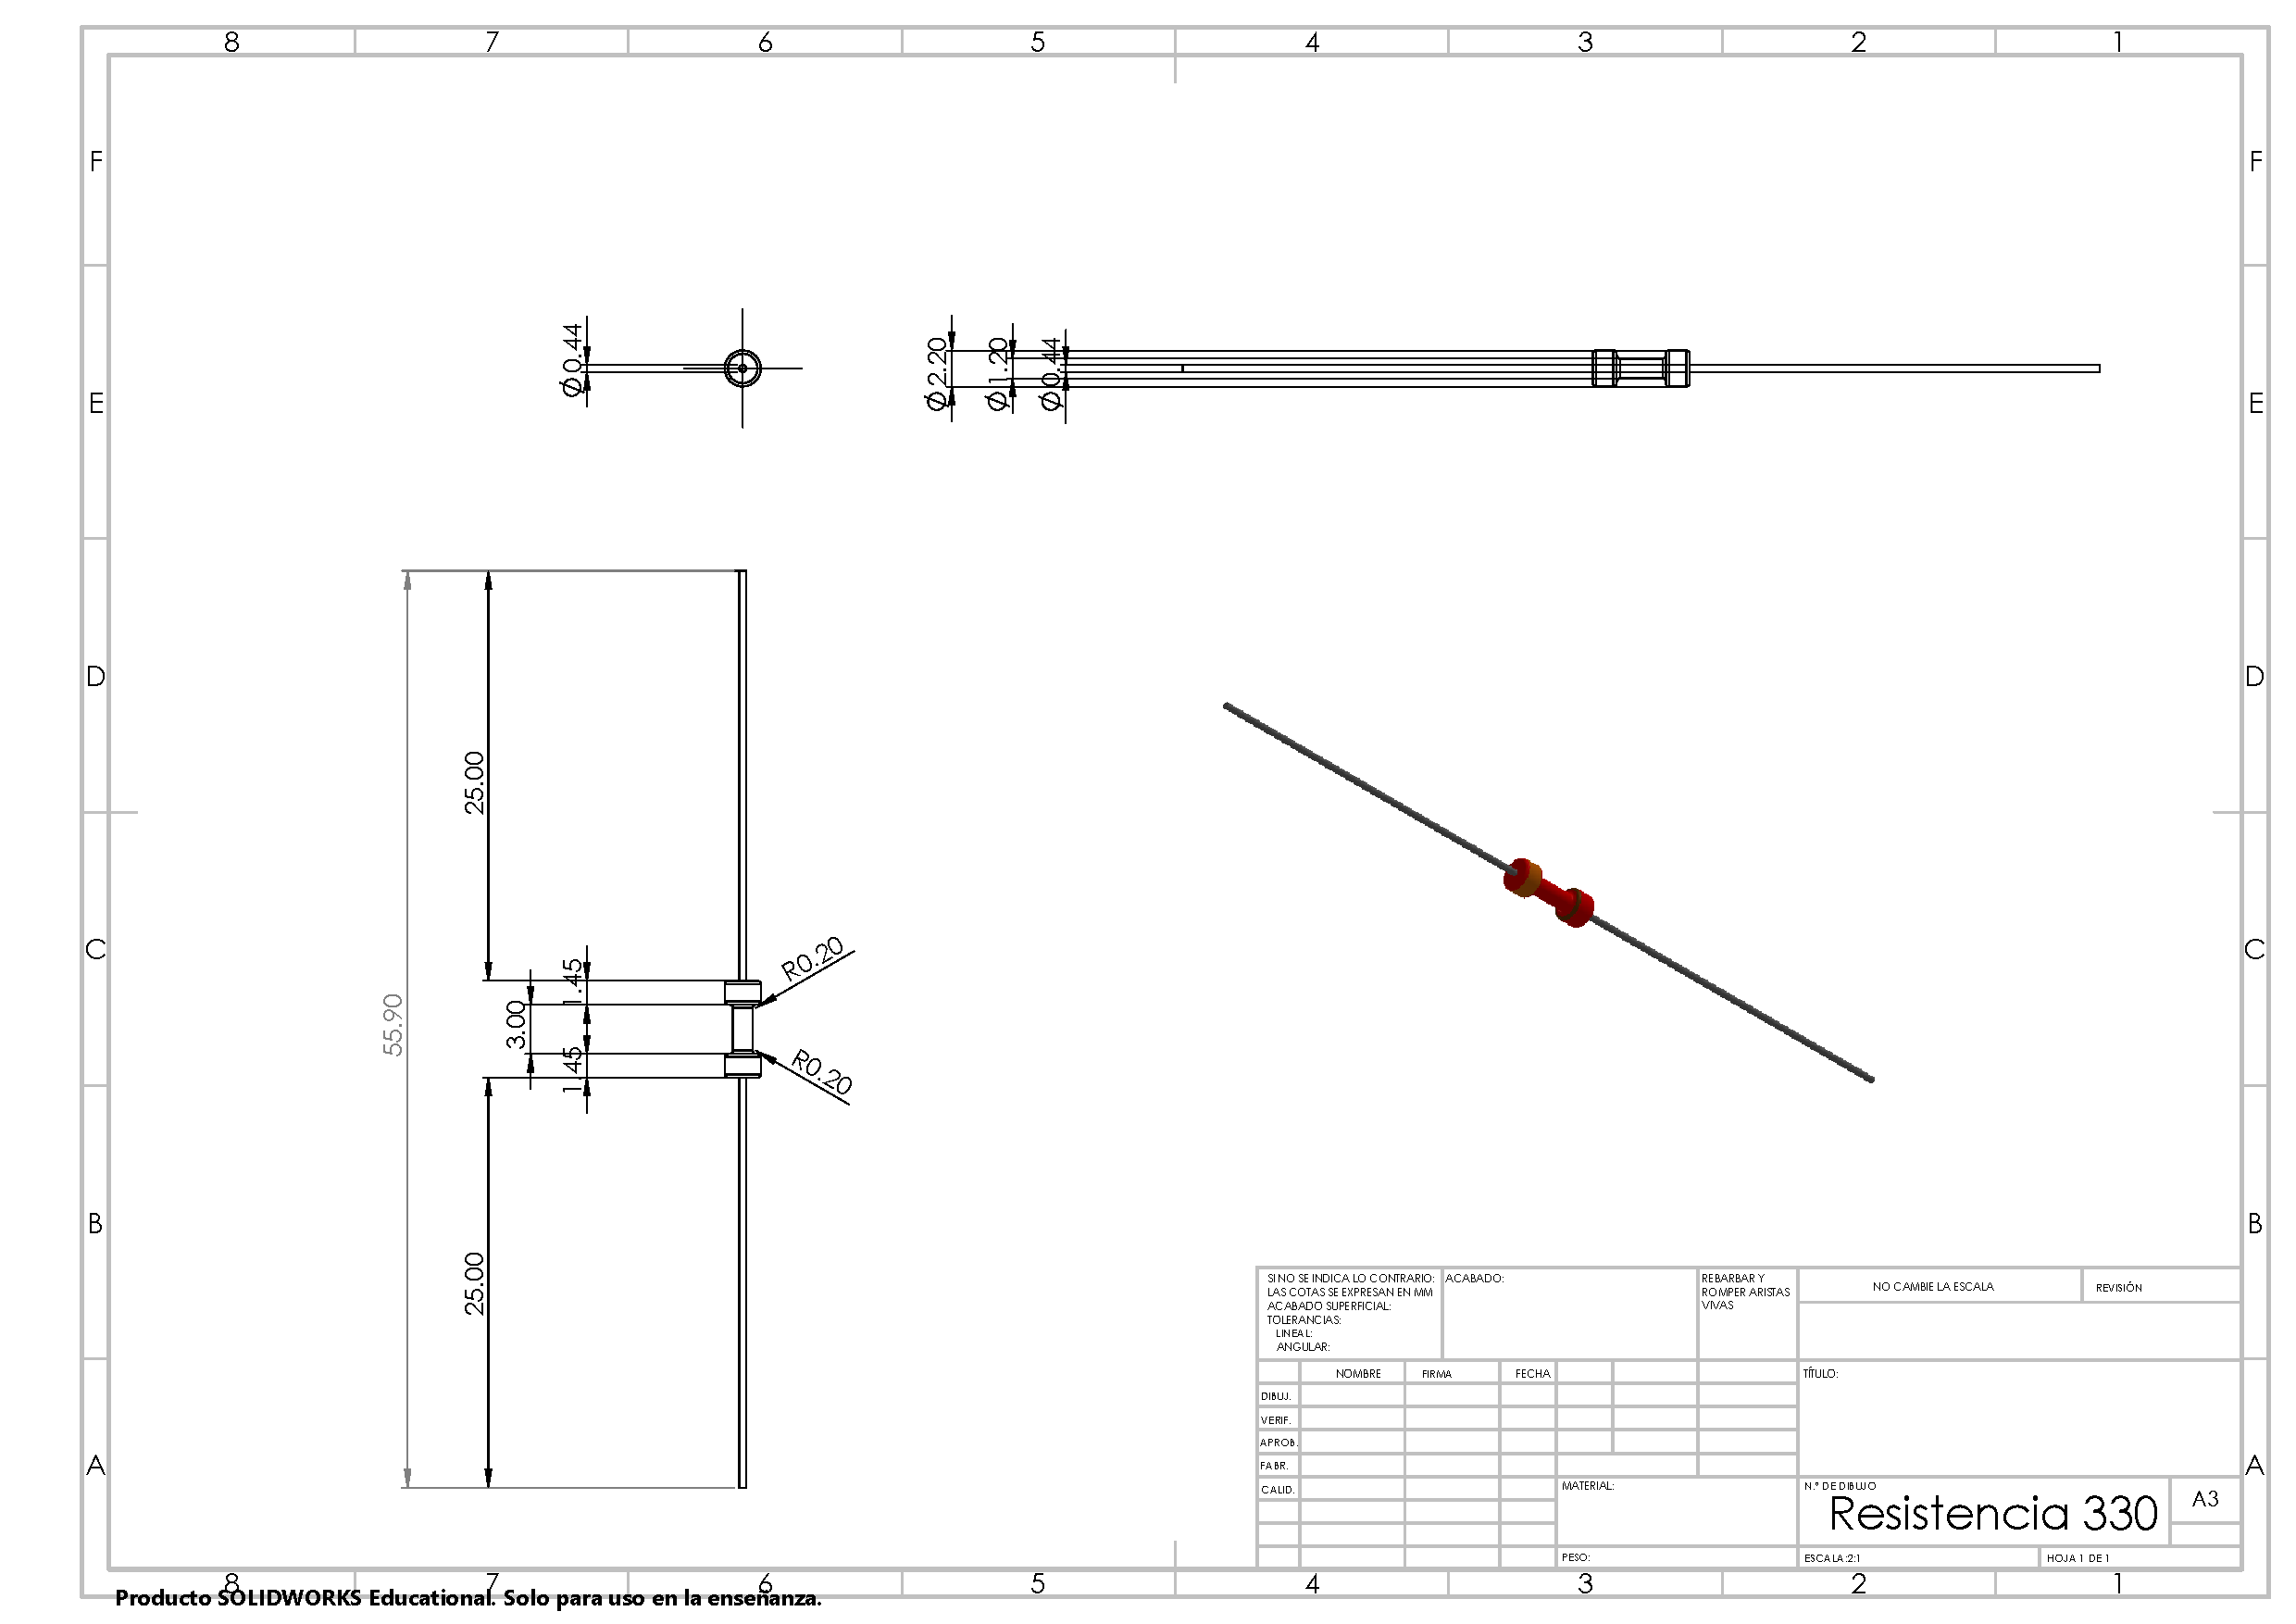
\includepdf[pages=-]{16/Img/resistencia330}
%%%%%%%%%%%%%%%%%%%%%%%%%%%%%%%%%%
%\centering{\section[\appendixautorefname{}]{Apéndice}}\label{anexo:tablaDeRegistro}
%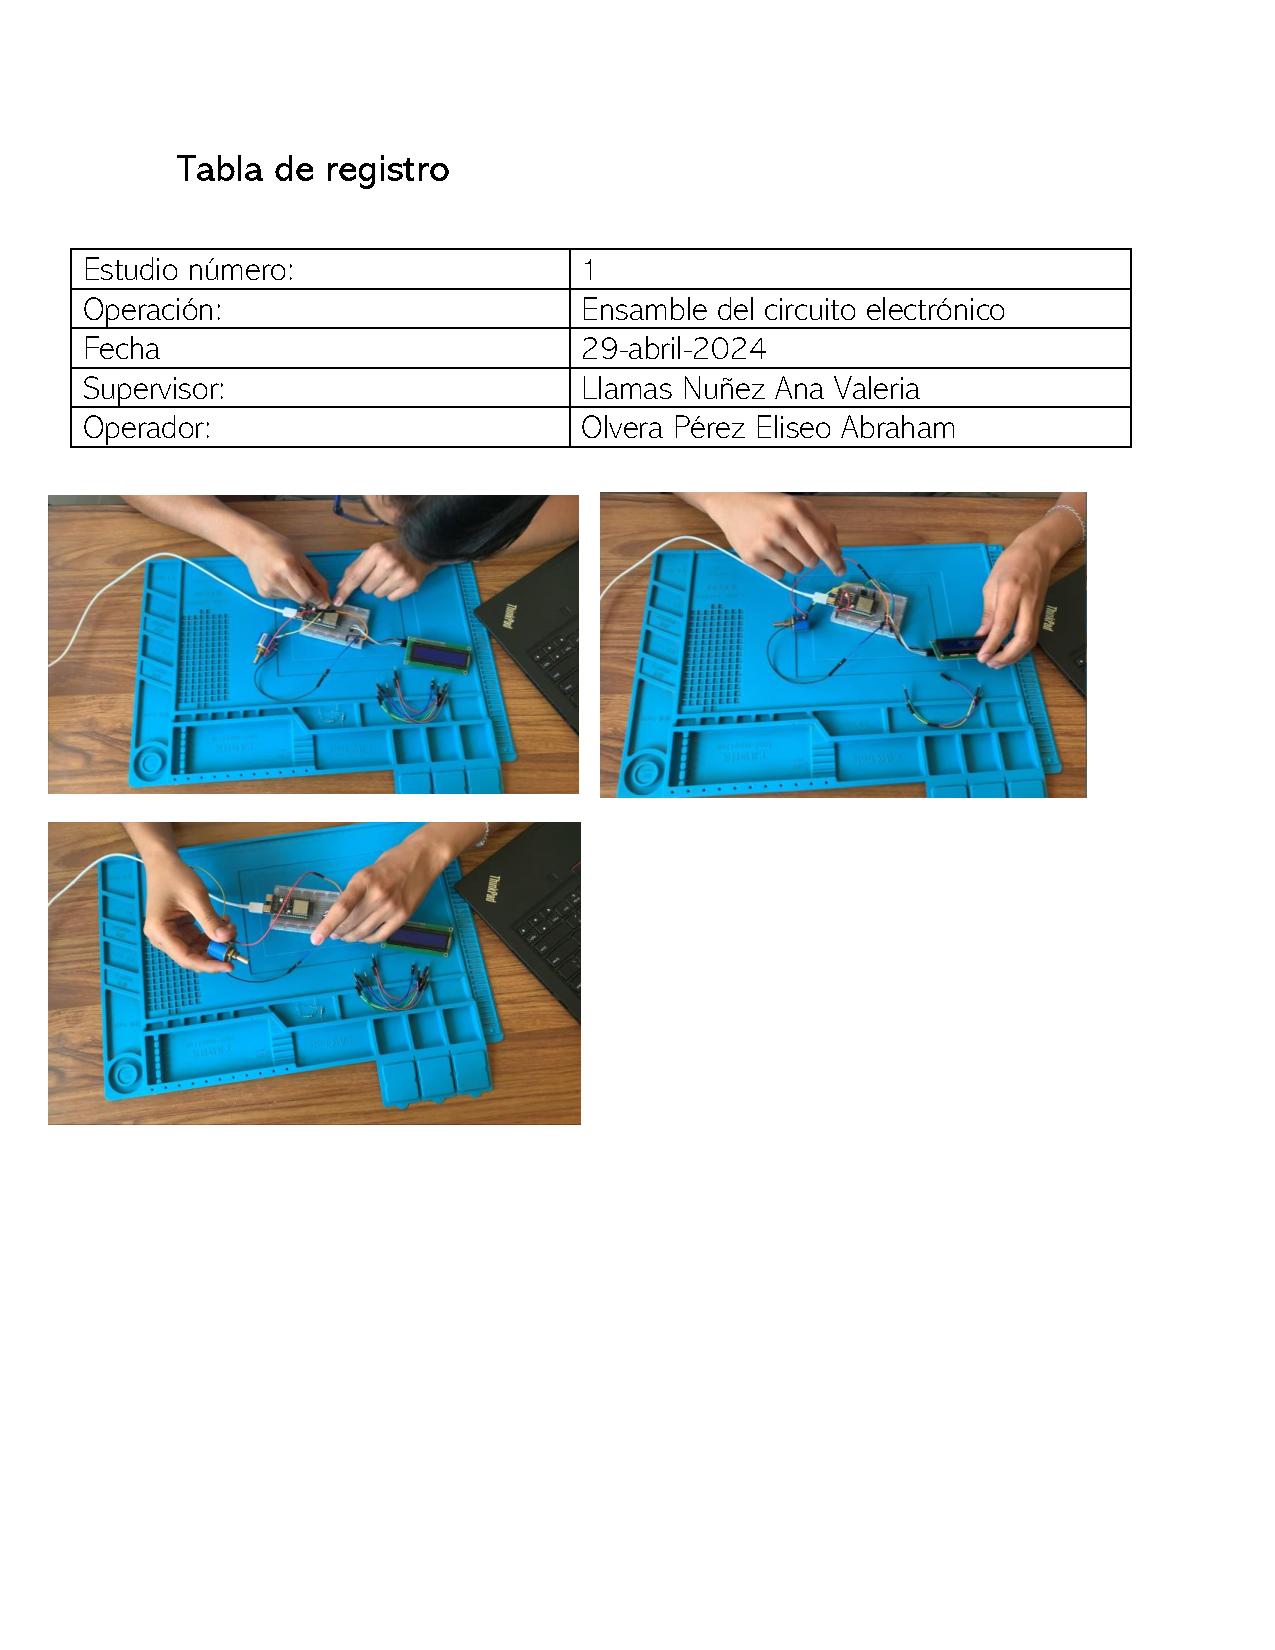
\includepdf[pages=-]{16/Img/tablaDeRegistro}
%%%%%%%%%%%%%%%%%%%%%%%%%%%%%%%%%%